%%%%%%%%%%%%%%%%%%%%%%%%%%%%%%%%%%%%%%%%%%%%%%%%%%%%%%%%%%%%%%%%%%%%%%
% Overleaf (WriteLaTeX) Example: Molecular Chemistry Presentation
%
% Source: http://www.overleaf.com
%
% In these slides we show how Overleaf can be used with standard 
% chemistry packages to easily create professional presentations.
% 
% Feel free to distribute this example, but please keep the referral
% to overleaf.com
% 
%%%%%%%%%%%%%%%%%%%%%%%%%%%%%%%%%%%%%%%%%%%%%%%%%%%%%%%%%%%%%%%%%%%%%%

\documentclass{beamer}

\mode<presentation>
{
  \usetheme{Madrid}       % or try default, Darmstadt, Warsaw, ...
  \usecolortheme{default} % or try albatross, beaver, crane, ...
  \usefonttheme{default}    % or try default, structurebold, ...
  \setbeamertemplate{navigation symbols}{}
  \setbeamertemplate{caption}[numbered]
} 

\usepackage[english]{babel}
\usepackage[utf8x]{inputenc}
\usepackage{graphicx}
\usepackage{hyperref}
  \hypersetup{colorlinks=true}
  \hypersetup{urlcolor=blue}
  \hypersetup{linkcolor = .}
\usepackage{xcolor}
\usepackage{siunitx}
  \sisetup{separate-uncertainty = true}
\usepackage{physics}
\usepackage[font=small,labelfont=bf]{caption}
\usepackage{subcaption}
\usepackage[en-GB]{datetime2}
\usepackage{overpic}
\usepackage{feynmp}
\DeclareGraphicsRule{*}{mps}{*}{}
\usepackage{scalerel}
\newcommand{\mylbrace}[2]{\vspace{#2pt}\hspace{6pt}\scaleleftright[\dimexpr5pt+#1\dimexpr0.06pt]{\lbrace}{\rule[\dimexpr2pt-#1\dimexpr0.5pt]{-4pt}{#1pt}}{.}}
\newcommand{\myrbrace}[2]{\vspace{#2pt}\scaleleftright[\dimexpr5pt+#1\dimexpr0.06pt]{.}{\rule[\dimexpr2pt-#1\dimexpr0.5pt]{-4pt}{#1pt}}{\rbrace}\hspace{6pt}}

% Trim in percent
\usepackage{adjustbox}

% No "Figure" prefix
\setbeamertemplate{caption}{\raggedright\insertcaption\par}

% Nice decay amplitude diagrams
\usepackage{amsmath,amssymb,tikz-cd}

% Strike out text
\usepackage[normalem]{ulem}

% For figures with text overlay
\usepackage{overpic}

% Here's where the presentation starts, with the info for the title slide
\title[$B^\pm\to{[K^+K^-\pi^+\pi^-]}_Dh^\pm$]{Model independent measurement of the CKM angle \texorpdfstring{$\gamma$}{gamma} with \texorpdfstring{$B^\pm\to[K^+K^-\pi^+\pi^-]_Dh^\pm$}{B2DhD2KKpipi} at LHCb and BESIII}

\author{Martin Tat}
\institute[University of Oxford]{\normalsize University of Oxford\\ \vspace{0.3cm}\normalsize Warwick EPP Seminar}
\date{9th February 2023}

\titlegraphic{
\includegraphics[height = 2cm]{lhcb.jpg}\hspace{1cm}~%
              
\includegraphics[height = 2cm]{OxfordLogo.pdf}\hspace{1cm}~%
              
\includegraphics[height = 2cm]{bes3.jpg}}

\begin{document}

\begin{frame}
  \titlepage
\end{frame}

% These three lines create an automatically generated table of contents.
% \begin{frame}{Outline}
%   \tableofcontents
% \end{frame}

\section{Introduction to \texorpdfstring{$C\!P$}{CP} violation}
\begin{frame}{Introduction to $C\!P$ violation}
  \begin{center}
    {\huge Introduction to $C\!P$ violation}
  \end{center}
\end{frame}

\begin{frame}{Big Bang and matter-antimatter asymmetry}
  \begin{figure}
    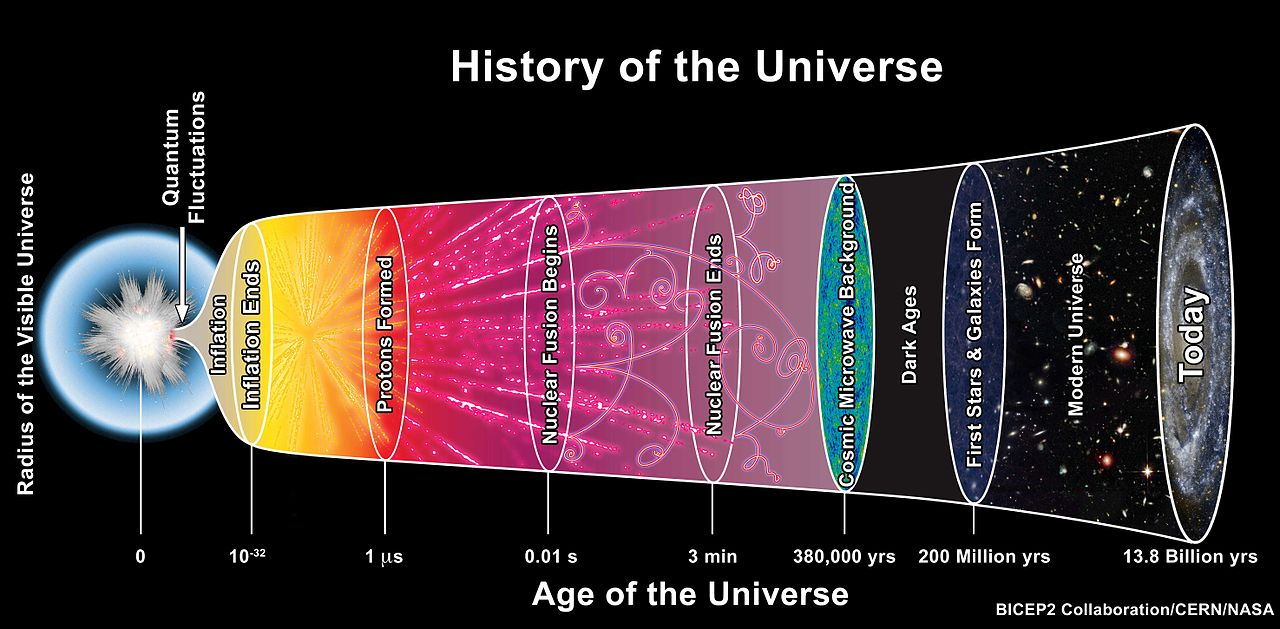
\includegraphics[height=5.5cm]{Plots/BigBangHistory.jpg}
  \end{figure}
  \begin{center}
    \Large Where is the antimatter in the universe?
  \end{center}
\end{frame}

\begin{frame}{Big Bang and matter-antimatter asymmetry}
  \begin{figure}
    \adjustbox{trim={0} {0} {0.838\width} {0},clip=true}{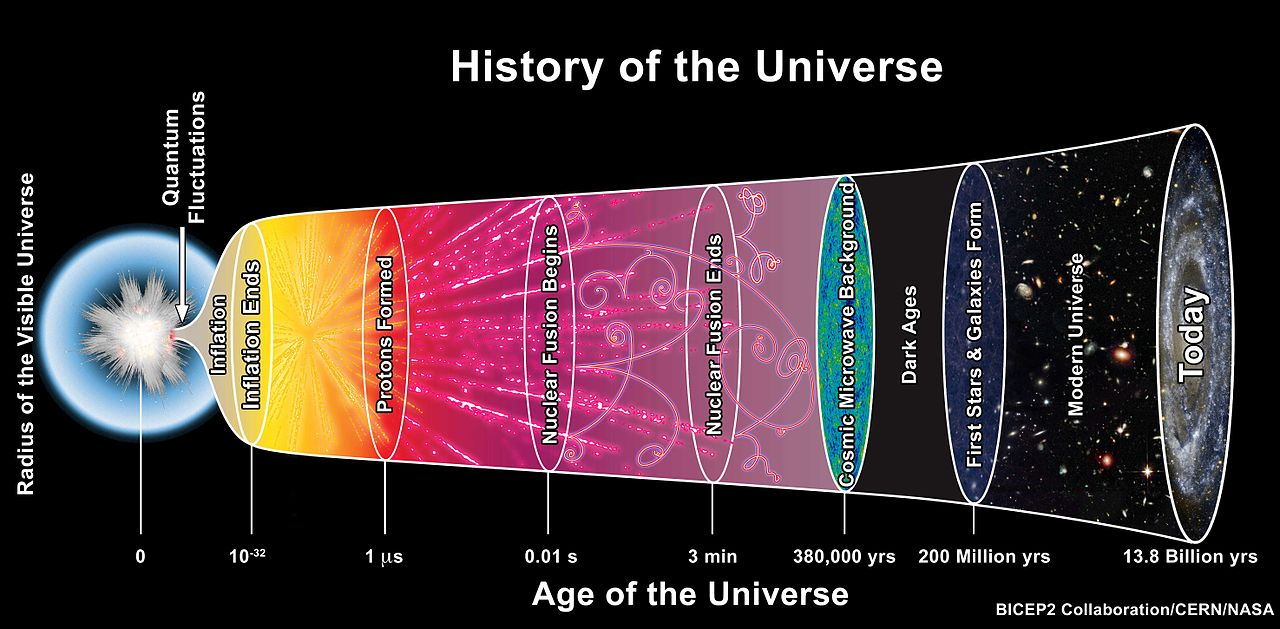
\includegraphics[height=5.5cm]{Plots/BigBangHistory.jpg}}%
    \adjustbox{trim={0.162\width} {0} {0} {0},clip=true}{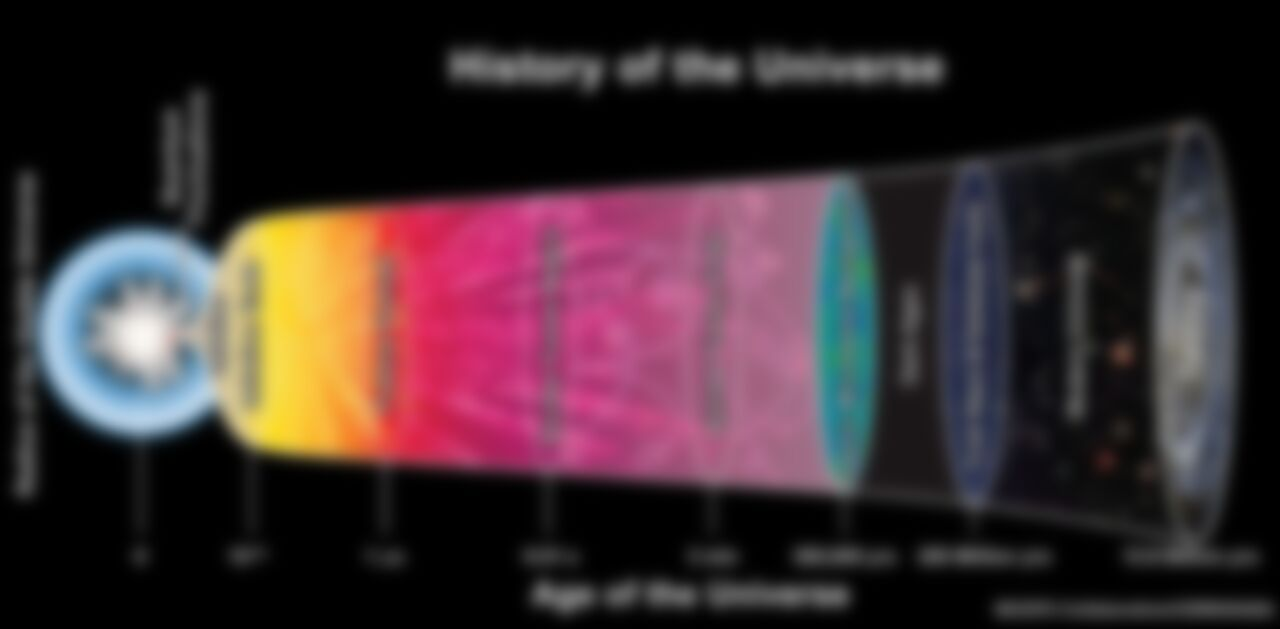
\includegraphics[height=5.5cm]{Plots/BigBangHistory_blur.jpg}}
  \end{figure}
  \begin{center}
    \Large Initially equal amounts of matter and antimatter...
  \end{center}
\end{frame}

\begin{frame}{Big Bang and matter-antimatter asymmetry}
  \begin{figure}
    \adjustbox{trim={0} {0} {0.18\width} {0},clip=true}{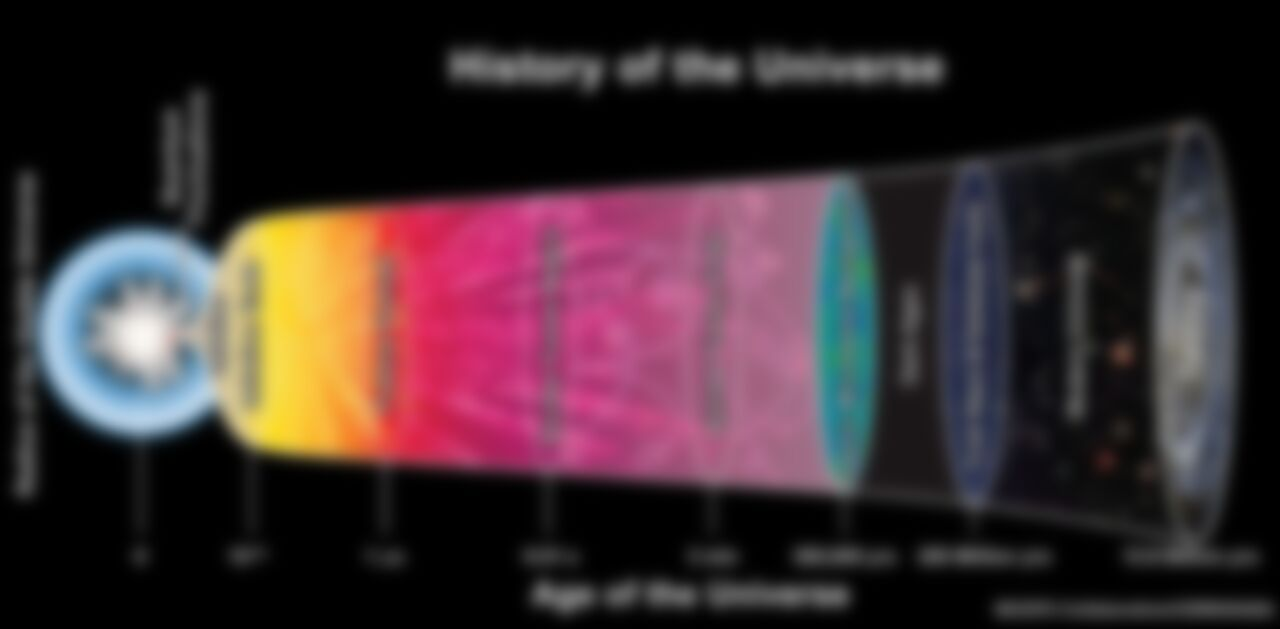
\includegraphics[height=5.5cm]{Plots/BigBangHistory_blur.jpg}}%
    \adjustbox{trim={0.82\width} {0} {0} {0},clip=true}{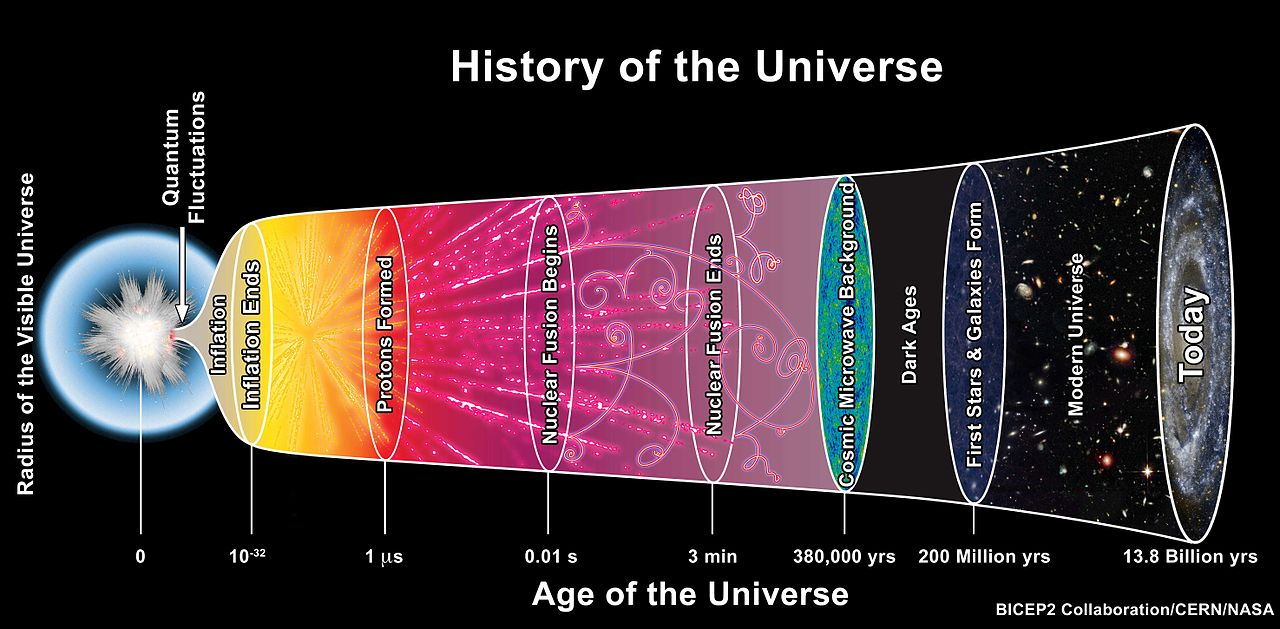
\includegraphics[height=5.5cm]{Plots/BigBangHistory.jpg}}
  \end{figure}
  \begin{center}
    \Large ... but today we only see matter!
  \end{center}
\end{frame}

\begin{frame}{Big Bang and matter-antimatter asymmetry}
  \begin{figure}
    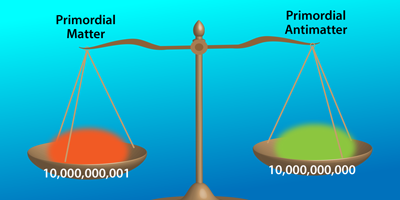
\includegraphics[width=0.8\textwidth,trim={0.9cm 0 0.9cm 0},clip=true]{Plots/PrimordialAntimatter.png}
    \caption*{\tiny APS/Alan Stonebraker}
  \end{figure}
  \vspace{-0.5cm}
  \begin{center}
    \Large The difference is very small...
  \end{center}
\end{frame}

\begin{frame}{Big Bang and matter-antimatter asymmetry}
  \begin{figure}
    
\includegraphics[width=0.45\textwidth]{Plots/MatterAntimatterBigAsymmetry.png}
    \caption*{\tiny Quantum Diaries: ``Why B physics? Why not A Physics?''}
  \end{figure}
  \vspace{-0.5cm}
  \begin{center}
    \Large ... but the effects we observe today are obviously huge! How can we explain this?
  \end{center}
\end{frame}

\begin{frame}{$C\!P$ violation}
  \begin{columns}
    \begin{column}{0.4\textwidth}
      \begin{figure}
        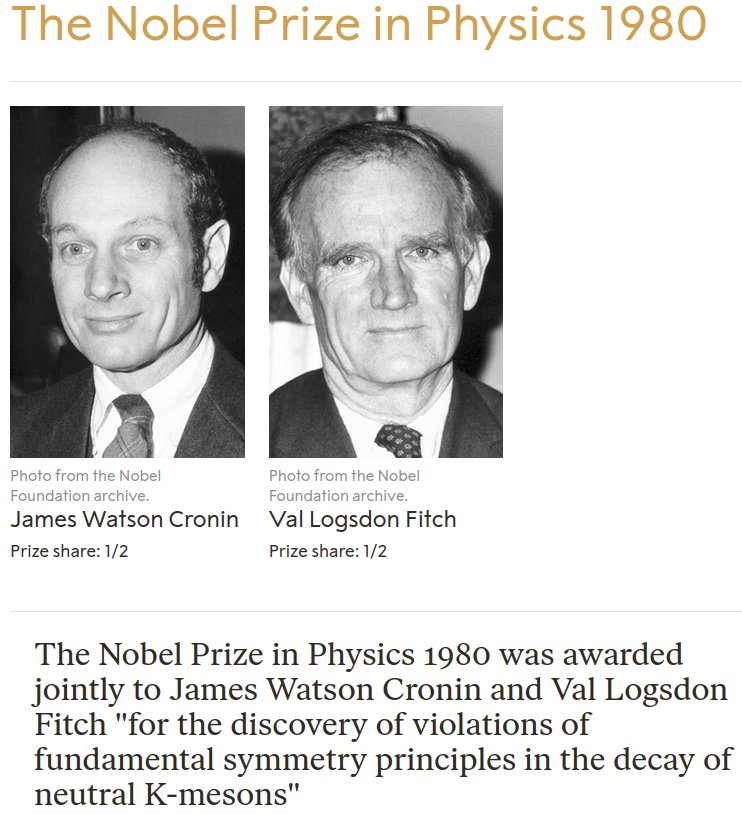
\includegraphics[width=1.0\textwidth]{Plots/NobelPrize1980.png}
      \end{figure}
    \end{column}
    \begin{column}{0.6\textwidth}
      \begin{itemize}
        \setlength\itemsep{1.0em}
        \item{$C\!P$ violation discovery in 1964}
        \item{Phys. Rev. Lett. \textbf{13}, 138}
        \item{Observed $K_L^0\to\pi^+\pi^-$}
        \item{Since, $C\!P$ violation has also been observed in the $B$, $B_s$ and $D$ systems}
      \end{itemize}
    \end{column}
  \end{columns}
  \vspace{0.5cm}
  \begin{center}
    \large Can Standard Model CPV explain the matter-antimatter asymmetry?\\Or, could it be physics beyond the SM?
  \end{center}
\end{frame}

\section{The CKM matrix and the Unitary Triangle}
\begin{frame}{The CKM matrix and the Unitary Triangle}
  \begin{center}
    {\huge The CKM matrix and the Unitary Triangle}
  \end{center}
\end{frame}

\begin{frame}{The CKM matrix and the Unitary Triangle}
  \begin{center}
    In SM, the charged current $W^\pm$ interactions couple (left-handed) up- and down-type quarks, given by
  \end{center}
  \begin{equation*}
    \frac{-g}{\sqrt{2}}
    \begin{bmatrix}
      \bar{u_L} & \bar{c_L} & \bar{t_L}
    \end{bmatrix}
    \gamma^\mu W_\mu V_{\rm CKM}
    \begin{bmatrix}
      d_L \\
      s_L \\
      b_L
    \end{bmatrix}
     + {\rm h.c.}
  \end{equation*}
  \begin{figure}[H]
    \centering
    \vspace{0.3cm}
    \begin{subfigure}{0.5\textwidth}
      \centering
      \begin{fmffile}{fgraph/fgraph_W1}
        \setlength{\unitlength}{0.4cm}
        \begin{fmfgraph*}(6,6)
          \fmfstraight
          \fmfleft{i1}
          \fmfright{o1,o2}
          \fmflabel{$t$}{i1}
          \fmflabel{$b$}{o1}
          \fmflabel{$W^+$}{o2}
          \fmf{fermion}{i1,v}
          \fmf{fermion}{v,o1}
          \fmf{boson}{v,o2}
        \end{fmfgraph*}
      \end{fmffile}
      \vspace{0.5cm}
      \caption{$t\to bW^+$}
    \end{subfigure}%
    \begin{subfigure}{0.5\textwidth}
      \centering
      \begin{fmffile}{fgraph/fgraph_W2}
        \setlength{\unitlength}{0.4cm}
        \begin{fmfgraph*}(6,6)
          \fmfstraight
          \fmfleft{i1}
          \fmfright{o1,o2}
          \fmflabel{$b$}{i1}
          \fmflabel{$c$}{o1}
          \fmflabel{$W^-$}{o2}
          \fmf{fermion}{i1,v}
          \fmf{fermion}{v,o1}
          \fmf{boson}{v,o2}
        \end{fmfgraph*}
      \end{fmffile}
      \vspace{0.5cm}
      \caption{$b\to cW^-$}
    \end{subfigure}
  \end{figure}
\end{frame}

\begin{frame}{The CKM matrix and the Unitary Triangle}
  \begin{center}
    The Cabbibo-Kobayashi-Maskawa matrix $V_{\rm CKM}$,
  \end{center}
  \begin{equation*}
    \begin{bmatrix}
      V_{ud} & V_{us} & V_{ub} \\
      V_{cd} & V_{cs} & V_{cb} \\
      V_{td} & V_{ts} & V_{tb}
    \end{bmatrix}
  \end{equation*}
  \begin{center}
    must be a unitary matrix: $V^\dagger_{\rm CKM}V_{\rm CKM} = I\implies$
  \end{center}
  \vspace{0.5cm}
  \begin{equation*}
    V^{\phantom{*}}_{ud}V^*_{ub} + V^{\phantom{*}}_{cd}V^*_{cb} + V^{\phantom{*}}_{td}V^*_{tb} = 0
  \end{equation*}
  \begin{center}
    Represent this constraint as a triangle in the complex plane:\\Unitary Triangle
  \end{center}
\end{frame}

\begin{frame}{The CKM matrix and the Unitary Triangle}
  \begin{itemize}
    \setlength\itemsep{0.3em}
    \item{CPV in SM is described by the Unitary Triangle, with angles $\alpha$, $\beta$, $\gamma$}
    \item{The angle $\gamma = \text{arg}\Big(-\frac{V^{\phantom{*}}_{ud}V^*_{ub}}{V^{\phantom{*}}_{cd}V^*_{cb}}\Big)$ is very important:}
    \begin{enumerate}
    \setlength\itemsep{0.2em}
      \item{Negligible theoretical uncertainties: Ideal SM benchmark}
      \item{Accessible at tree level: Indirectly probe New Physics that enter loops}
      \item{Compare with $\alpha$, $\beta$ measurements: Is the Unitary Triangle a triangle?}
    \end{enumerate}
  \end{itemize}
  \vspace{-0.2cm}
  \begin{figure}
    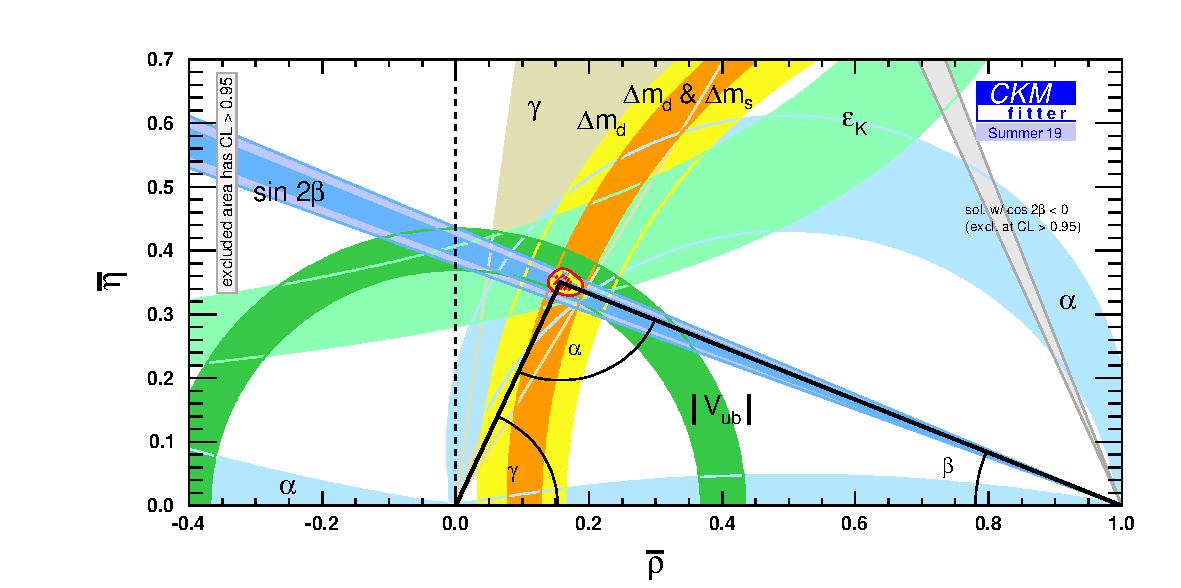
\includegraphics[width = 0.70\textwidth]{Plots/ckmfitter2.pdf}
    \vspace{-0.3cm}
    \caption*{\tiny CKMfitter Group (J. Charles et al.), Eur. Phys. J. C41, 1-131 (2005)}
  \end{figure}
\end{frame}

\section{How to measure \texorpdfstring{$\gamma$}{gamma}?}
\begin{frame}{How to measure $\gamma$?}
  \begin{center}
    {\huge How to measure $\gamma$?}
  \end{center}
\end{frame}

\begin{frame}{Sensitivity through interference}
  \begin{center}
    \Large Measure $\gamma$ through interference effects in $B^\pm\to DK^\pm$
  \end{center}
  \begin{figure}[H]
    \centering
    \begin{subfigure}{0.5\textwidth}
      \centering
      \begin{fmffile}{fgraph/fgraph_BtoDK1}
        \setlength{\unitlength}{0.4cm}
        \begin{fmfgraph*}(6,6)
          \fmfstraight
          \fmfleft{i1,B,i2,t1,t2,t3,t9,t10}
          \fmfright{o1,D,o2,t4,t5,o3,K,o4}
          \fmflabel{$\bar{u}$}{i1}
          \fmflabel{$b$}{i2}
          \fmfv{l.d=20,l.a=180,l={$B^-$\mylbrace{30}{-8}}}{B}
          \fmflabel{$\bar{u}$}{o1}
          \fmflabel{$c$}{o2}
          \fmflabel{$\bar{u}$}{o3}
          \fmflabel{$s$}{o4}
          \fmfv{l.d=15,l.a=0,l={\myrbrace{30}{-12}}$D^0$}{D}
          \fmfv{l.d=15,l.a=0,l={\myrbrace{30}{11}}$K^-$}{K}
          \fmf{fermion}{o1,i1}
          \fmf{fermion,tension=1.5}{i2,v1}
          \fmf{fermion}{v1,o2}
          \fmf{phantom,tension=1.5}{t9,v2}
          \fmf{boson,label=$W$,label.side=left,tension=0}{v1,v2}
          \fmf{fermion}{v2,o4}
          \fmf{fermion}{o3,v2}
        \end{fmfgraph*}
      \end{fmffile}
      \vspace{0.5cm}
      \caption*{Favoured $B^-\to D^0K^-$}
    \end{subfigure}%
    \begin{subfigure}{0.5\textwidth}
      \centering
      \begin{fmffile}{fgraph/fgraph_BtoDK2}
        \setlength{\unitlength}{0.4cm}
        \begin{fmfgraph*}(6,6)
          \fmfstraight
          \fmfleft{i1,t1,t2,B,t9,t10,i2}
          \fmfright{o1,K,o2,t4,t5,o3,D,o4}
          \fmflabel{$\bar{u}$}{i1}
          \fmflabel{$b$}{i2}
          \fmfv{l.d=20,l.a=180,l={$B^-$\mylbrace{100}{-8}}}{B}
          \fmflabel{$\bar{u}$}{o1}
          \fmflabel{$s$}{o2}
          \fmflabel{$\bar{c}$}{o3}
          \fmflabel{$u$}{o4}
          \fmfv{l.d=15,l.a=0,l={\myrbrace{30}{13}}$\bar{D^0}$}{D}
          \fmfv{l.d=15,l.a=0,l={\myrbrace{30}{-13}}$K^-$}{K}
          \fmf{fermion}{o1,i1}
          \fmf{fermion,tension=1.5}{i2,v1}
          \fmf{fermion}{v1,o4}
          \fmf{phantom,tension=1.5}{t2,v2}
          \fmf{boson,label=$W$,label.side=left,tension=0}{v1,v2}
          \fmf{fermion}{v2,o2}
          \fmf{fermion}{o3,v2}
        \end{fmfgraph*}
      \end{fmffile}
      \vspace{0.5cm}
      \caption*{Suppressed $B^-\to\bar{D^0}K^-$}
    \end{subfigure}
  \end{figure}
  \vspace{-0.3cm}
  \begin{itemize}
    \item{Superposition of $D^0$ and $\bar{D^0}$}
    \item{$b\to u\bar{c}s$ and $b\to c\bar{u}s$ interference $\to$ Sensitivity to $\gamma$}
  \end{itemize}
  \vspace{-0.3cm}
  \begin{center}
    $\mathcal{A}(B^-)=\mathcal{A}_B\Big(\mathcal{A}_{D^0} + r_Be^{i(\delta_B - \gamma)}\mathcal{A}_{\bar{D^0}}\Big)$ \\
    $\mathcal{A}(B^+)=\mathcal{A}_B\Big(\mathcal{A}_{\bar{D^0}} + r_Be^{i(\delta_B + \gamma)}\mathcal{A}_{D^0}\Big)$ \\
  \end{center}
  \vspace{-0.3cm}
  \begin{itemize}
    \item{The magnitude of interference effects governed by $r_B\approx0.1$}
  \end{itemize}
\end{frame}

\begin{frame}[fragile]{$D$ decays to a $C\!P$ eigenstate}
  \begin{center}
    A well known strategy is to consider $D$ decays to a $C\!P$ eigenstate\\~\\
    For $C\!P$ eigenstates, $\mathcal{A}_{D^0} = \mathcal{A}_{\bar{D^0}}$
  \end{center}
  \begin{equation*}
    \begin{tikzcd}[column sep=huge]
      & D^0K^- \arrow[dr, bend left = 25, "\mathcal{A}_{D^0}"] & \\
      B^- \arrow[ur, bend left, "\mathcal{A}_B"] \arrow[dr, bend right, "\mathcal{A}_B r_B e^{i(\delta_B - \gamma)}"'] & [5cm] & DK^- \\
      & \bar{D^0}K^- \arrow[ur, bend right = 25, "\mathcal{A}_{D^0}"'] & \\
    \end{tikzcd}
  \end{equation*}
  \begin{equation*}
    \lvert\mathcal{A}(B^-)\lvert^2\propto1 + r_B^2 + 2r_B\cos(\delta_B - \gamma)
  \end{equation*}
\end{frame}

\begin{frame}{$D$ decays to a $C\!P$ eigenstate}
  \begin{figure}
    \centering
    \begin{subfigure}{0.45\textwidth}
      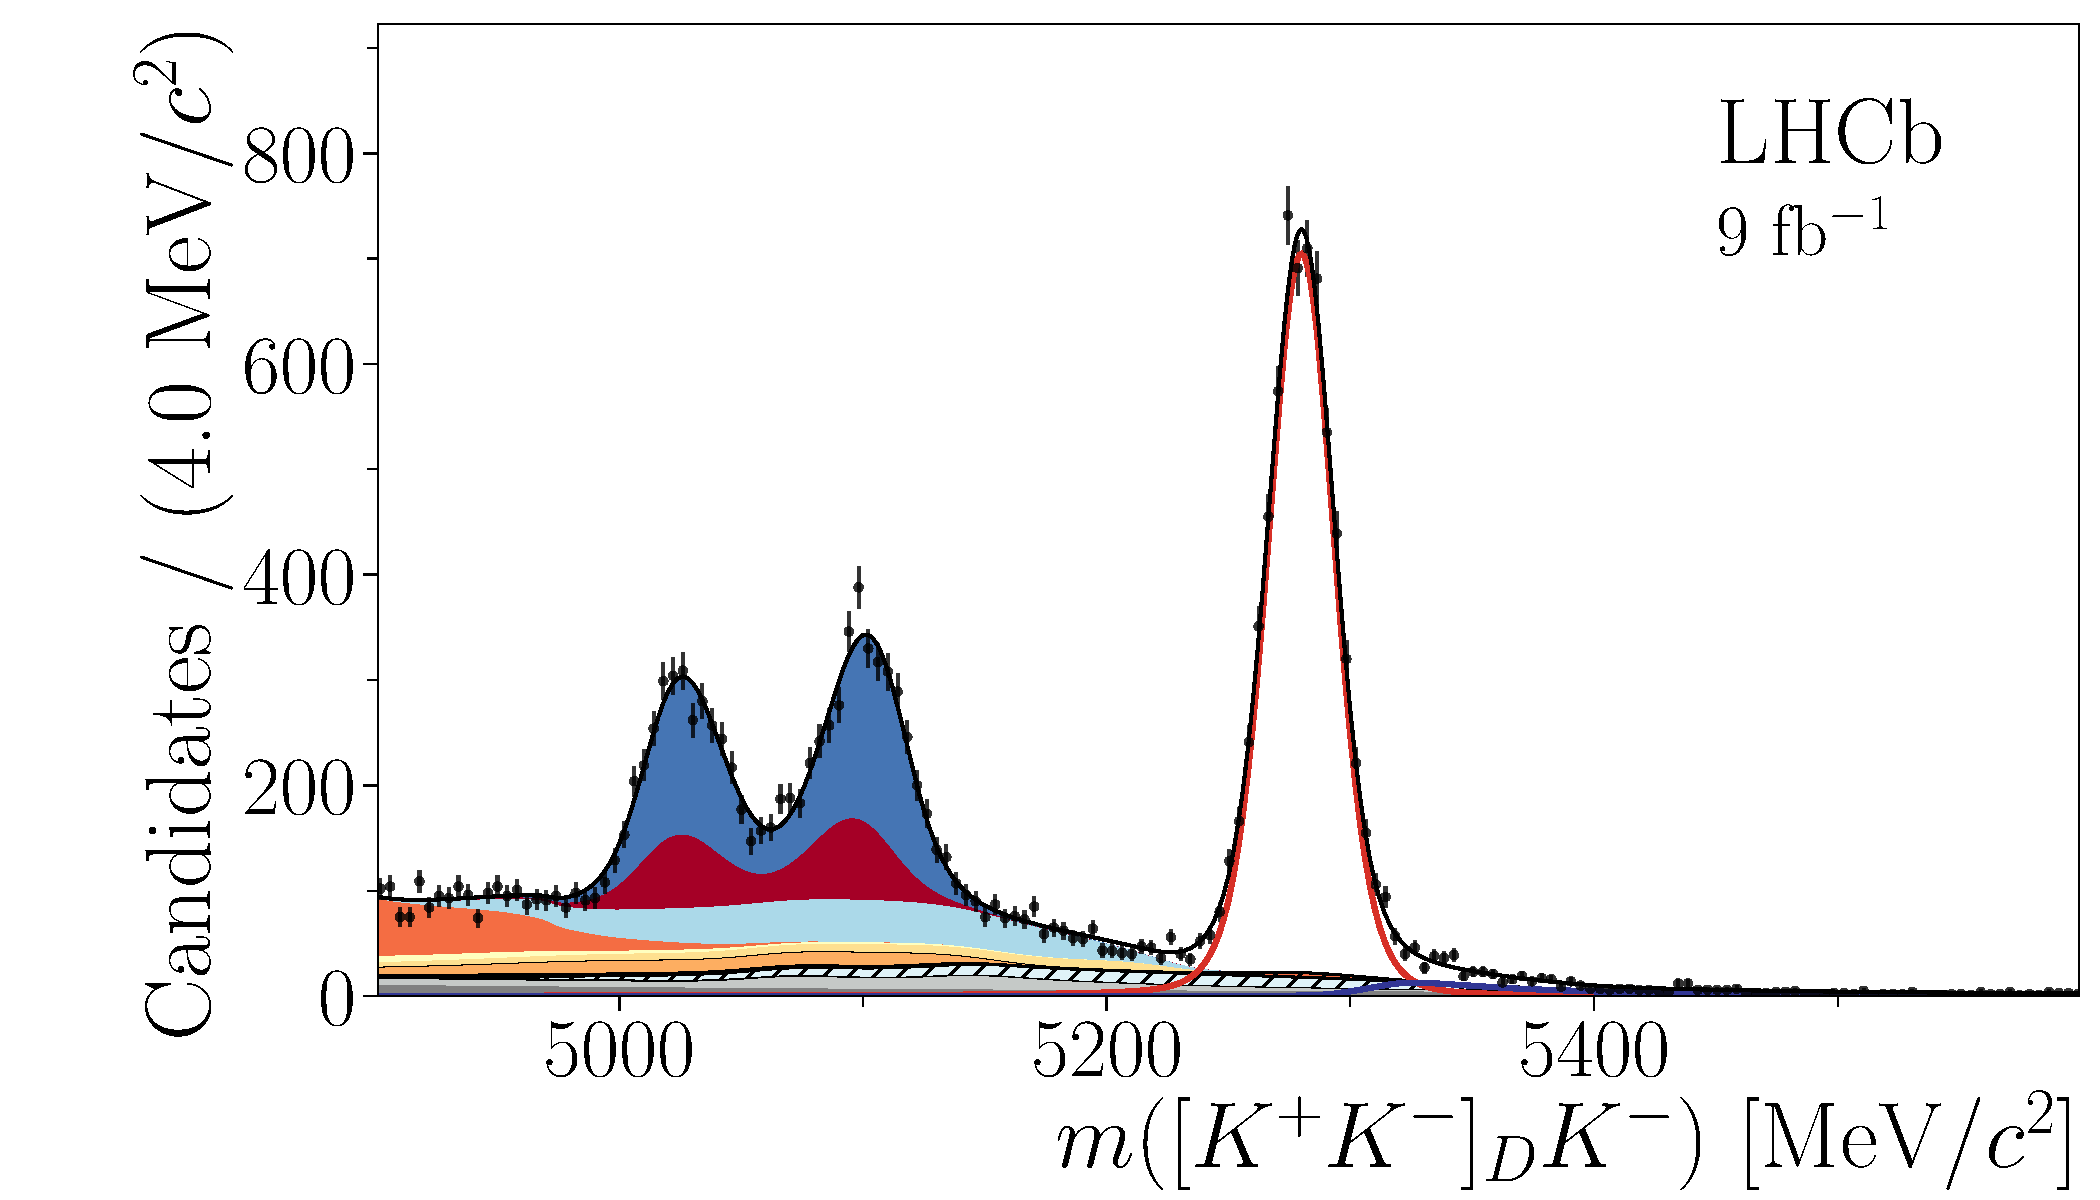
\includegraphics[width = 1.0\textwidth]{Plots/B2DK_D2KK_Minus.pdf}
    \end{subfigure}%
    \begin{subfigure}{0.45\textwidth}
      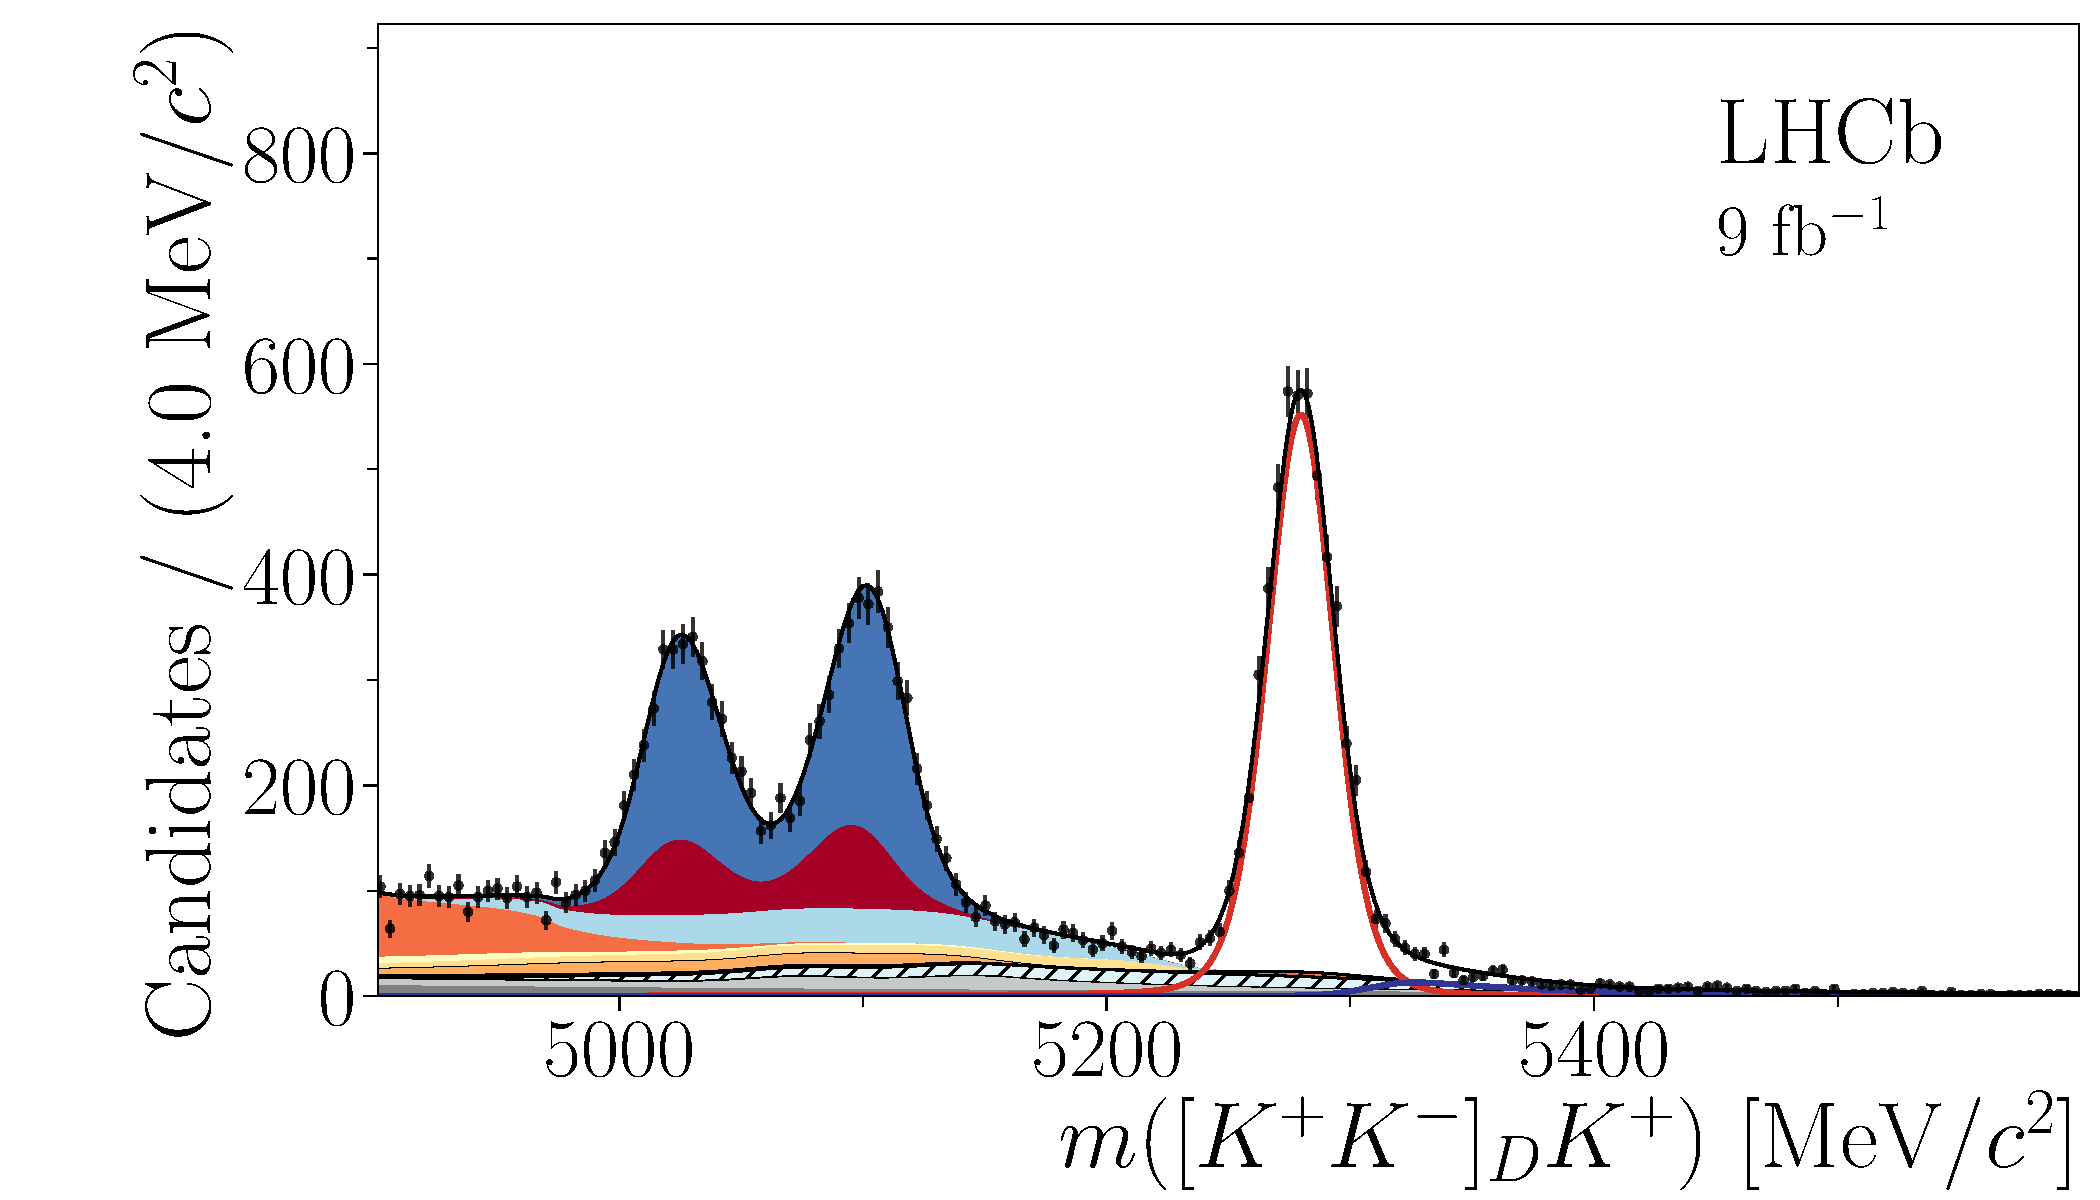
\includegraphics[width = 1.0\textwidth]{Plots/B2DK_D2KK_Plus.pdf}
    \end{subfigure}
    \begin{subfigure}{0.45\textwidth}
      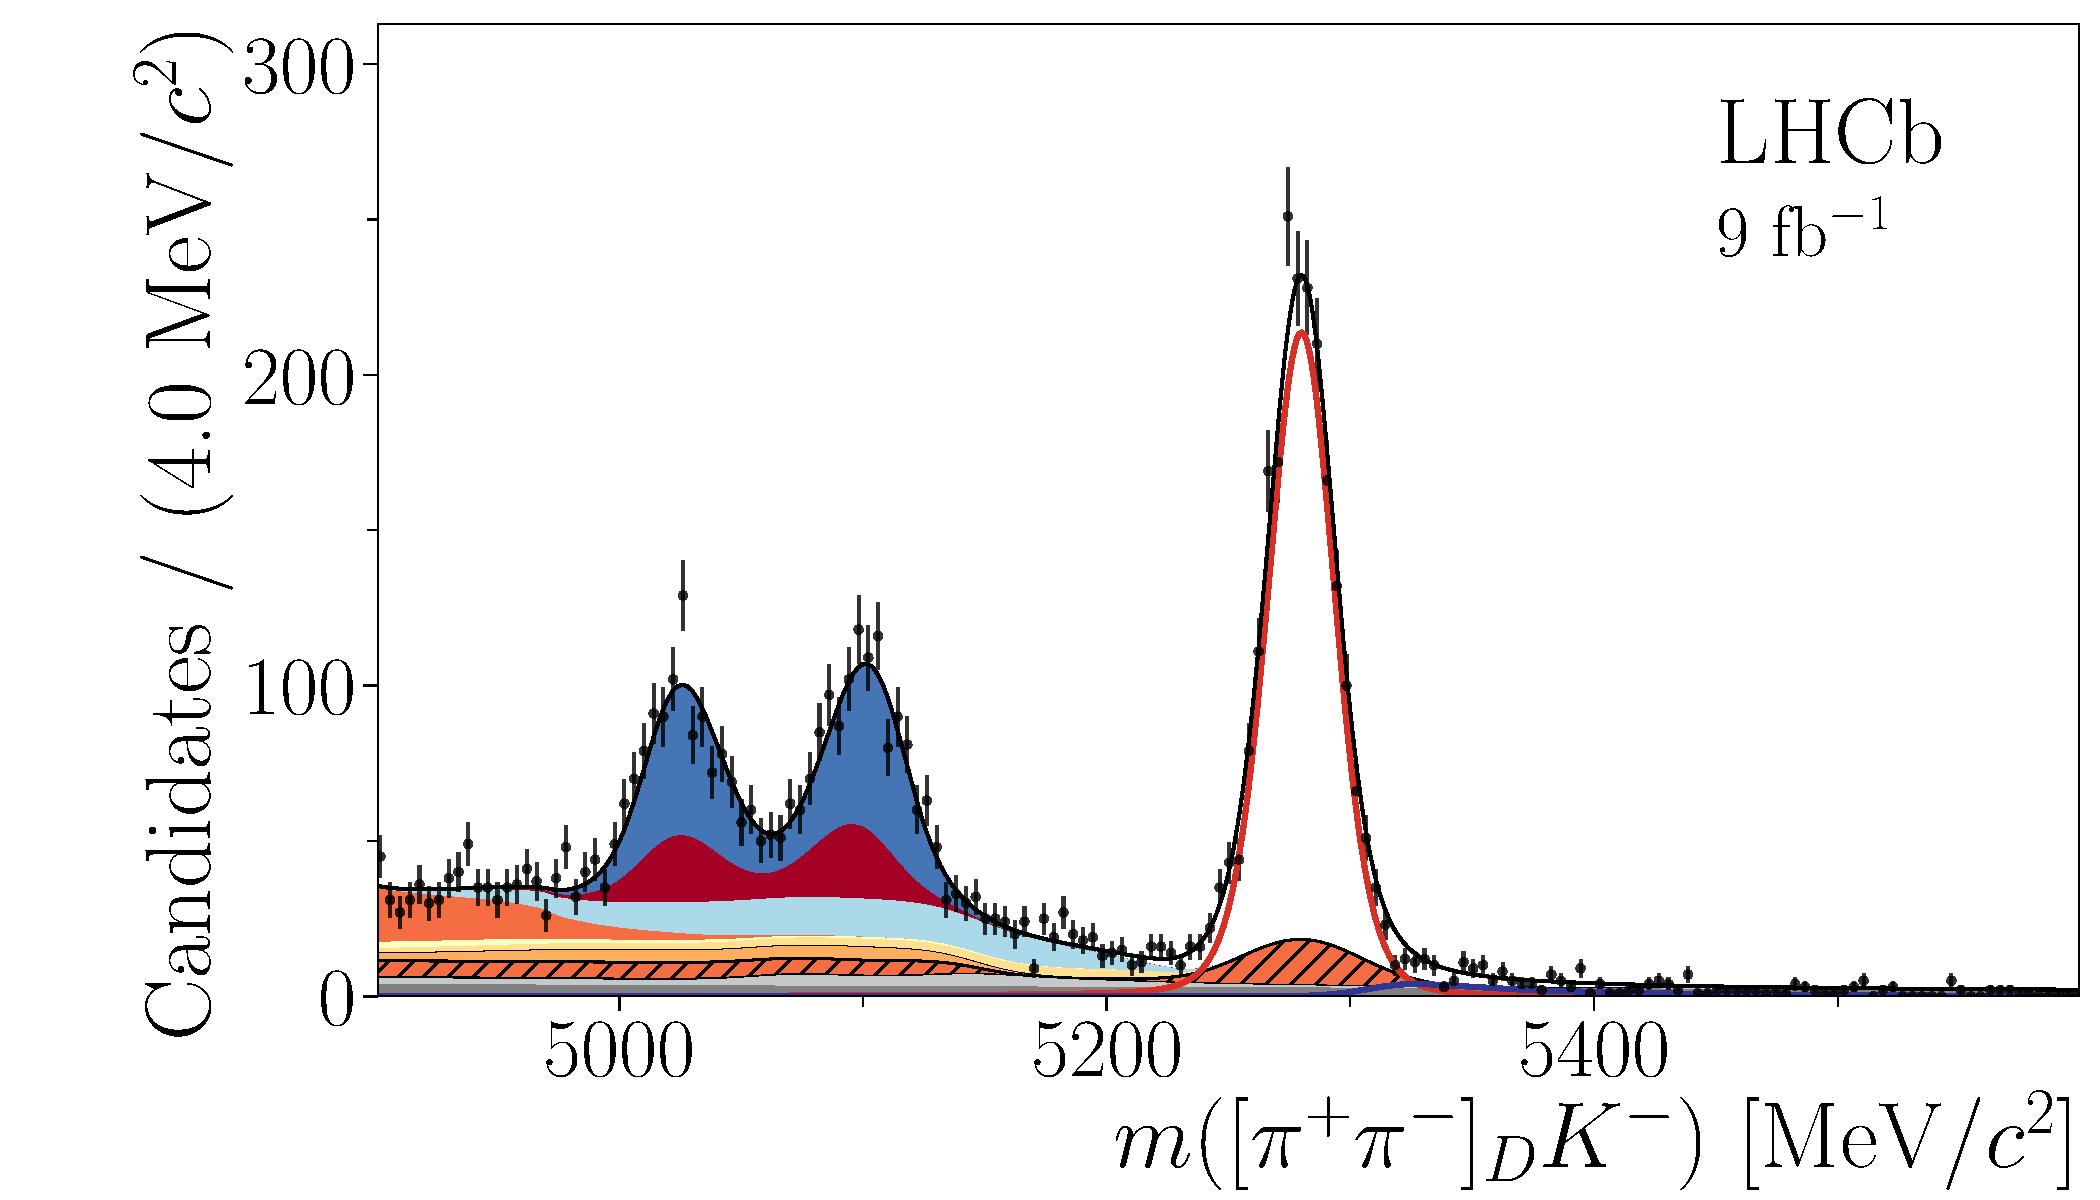
\includegraphics[width = 1.0\textwidth]{Plots/B2DK_D2pipi_Minus.pdf}
    \end{subfigure}%
    \begin{subfigure}{0.45\textwidth}
      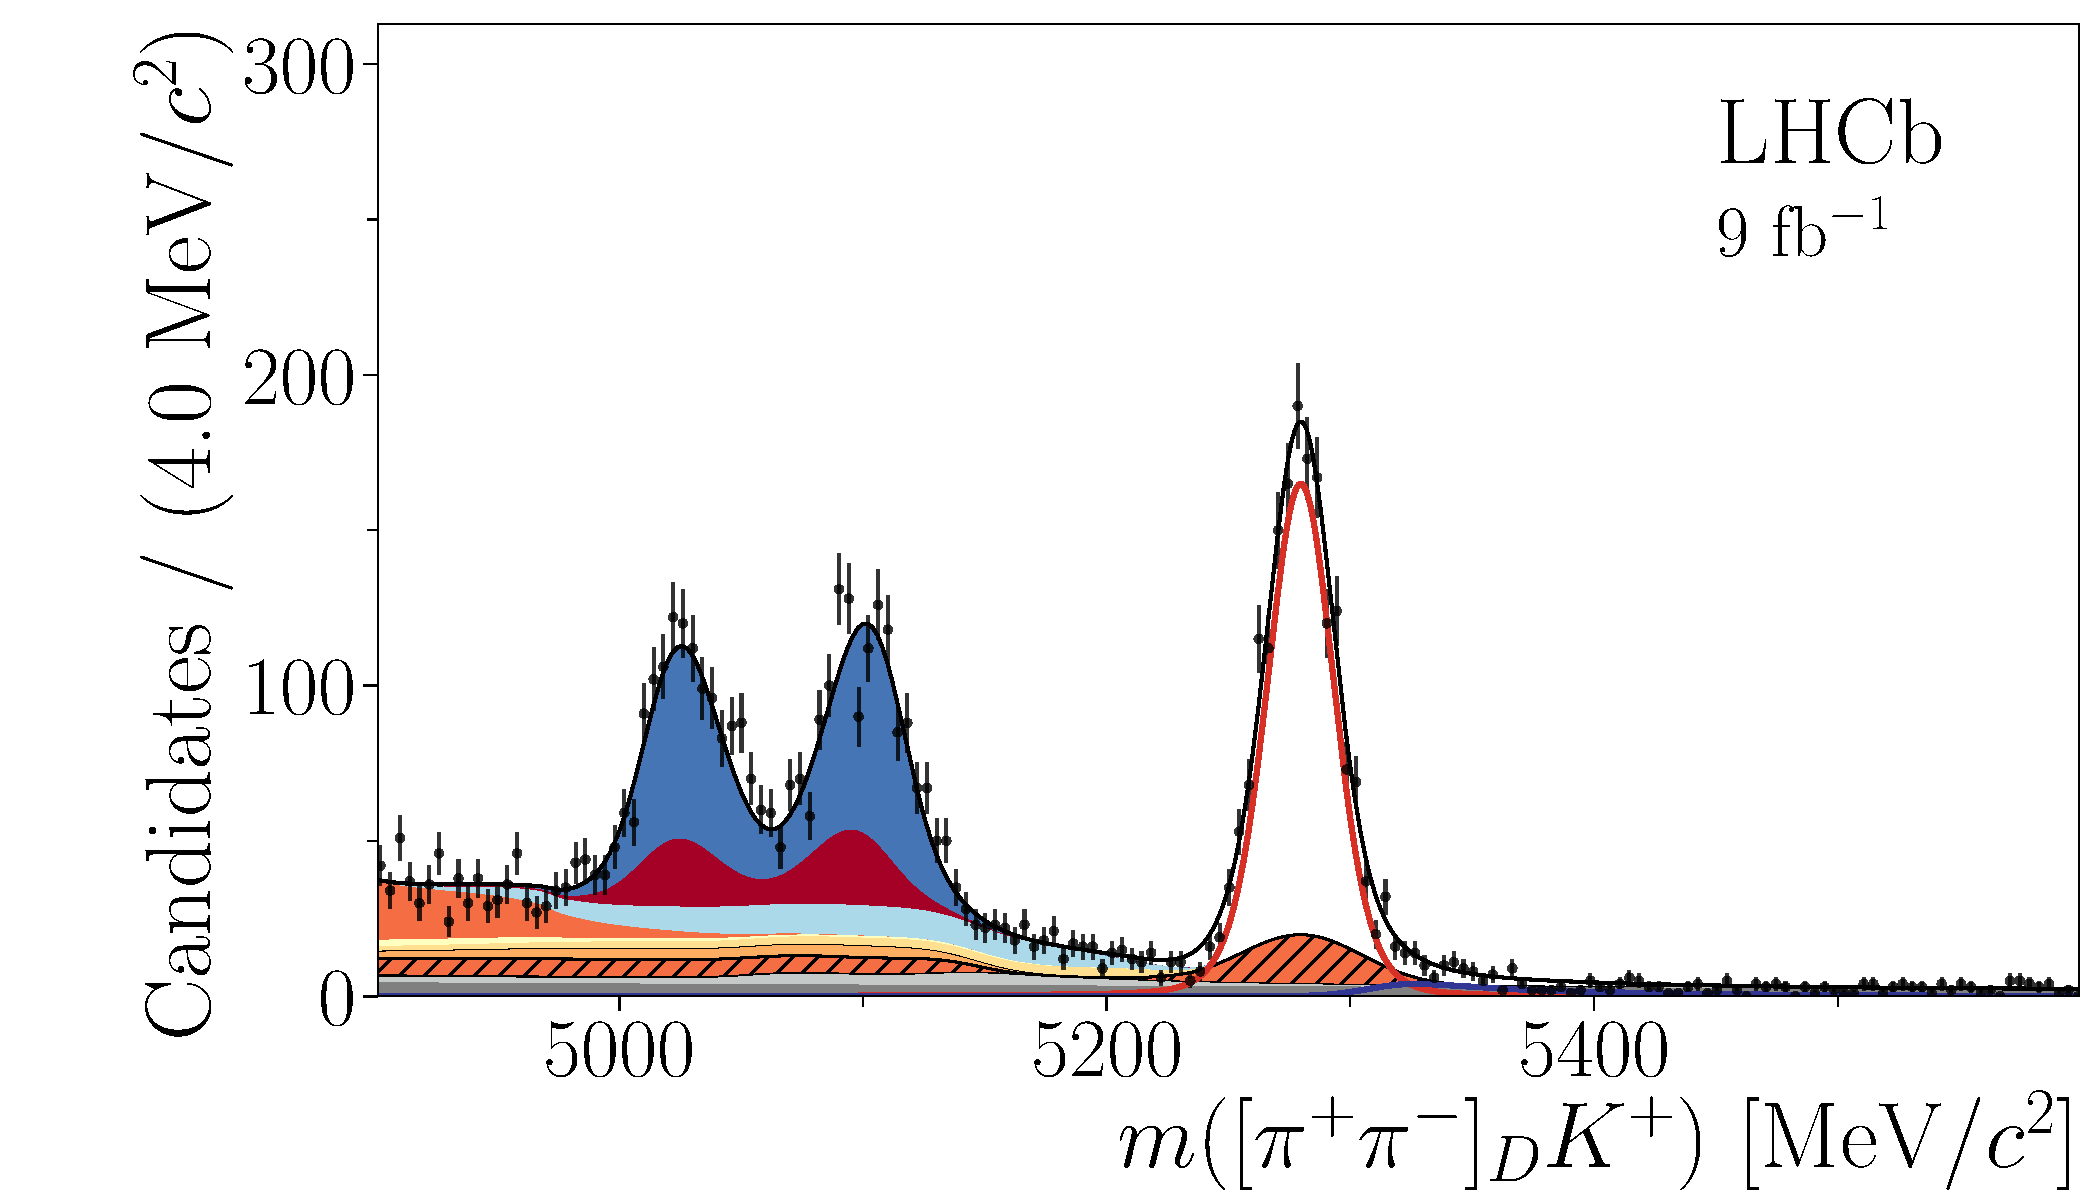
\includegraphics[width = 1.0\textwidth]{Plots/B2DK_D2pipi_Plus.pdf}
    \end{subfigure}
    \caption*{\tiny JHEP \textbf{04} (2021) 081}
  \end{figure}
  \vspace{-0.5cm}
  \begin{center}
    \Large In $B^\pm\to[h^+h^-]_DK^\pm$, we see significant CPV effects
  \end{center}
\end{frame}

\begin{frame}[fragile]{Doubly Suppressed Cabbibo $D$ decays}
  \begin{center}
    Can we enhance the interference effects?\\~\\
    Yes! Use a Doubly Suppressed Cabbibo decay: $\mathcal{A}_{D^0} = r_De^{i\delta_D}\mathcal{A}_{\bar{D^0}}$
  \end{center}
  \begin{equation*}
    \begin{tikzcd}[column sep=huge]
      & D^0K^- \arrow[dr, bend left = 25, "r_De^{i\delta_D}\mathcal{A}_{\bar{D^0}}"] & \\
      B^- \arrow[ur, bend left, "\mathcal{A}_B"] \arrow[dr, bend right, "\mathcal{A}_B r_B e^{i(\delta_B - \gamma)}"'] & [5cm] & DK^- \\
      & \bar{D^0}K^- \arrow[ur, bend right = 25, "\mathcal{A}_{\bar{D^0}}"'] & \\
    \end{tikzcd}
  \end{equation*}
  \begin{equation*}
    \lvert\mathcal{A}(B^-)\lvert^2\propto r_D^2 + r_B^2 + 2r_Br_D\cos(\delta_B - \gamma + \delta_D)
  \end{equation*}
\end{frame}

\begin{frame}{Doubly Suppressed Cabbibo $D$ decays}
  \begin{figure}
    \centering
    \begin{subfigure}{0.5\textwidth}
      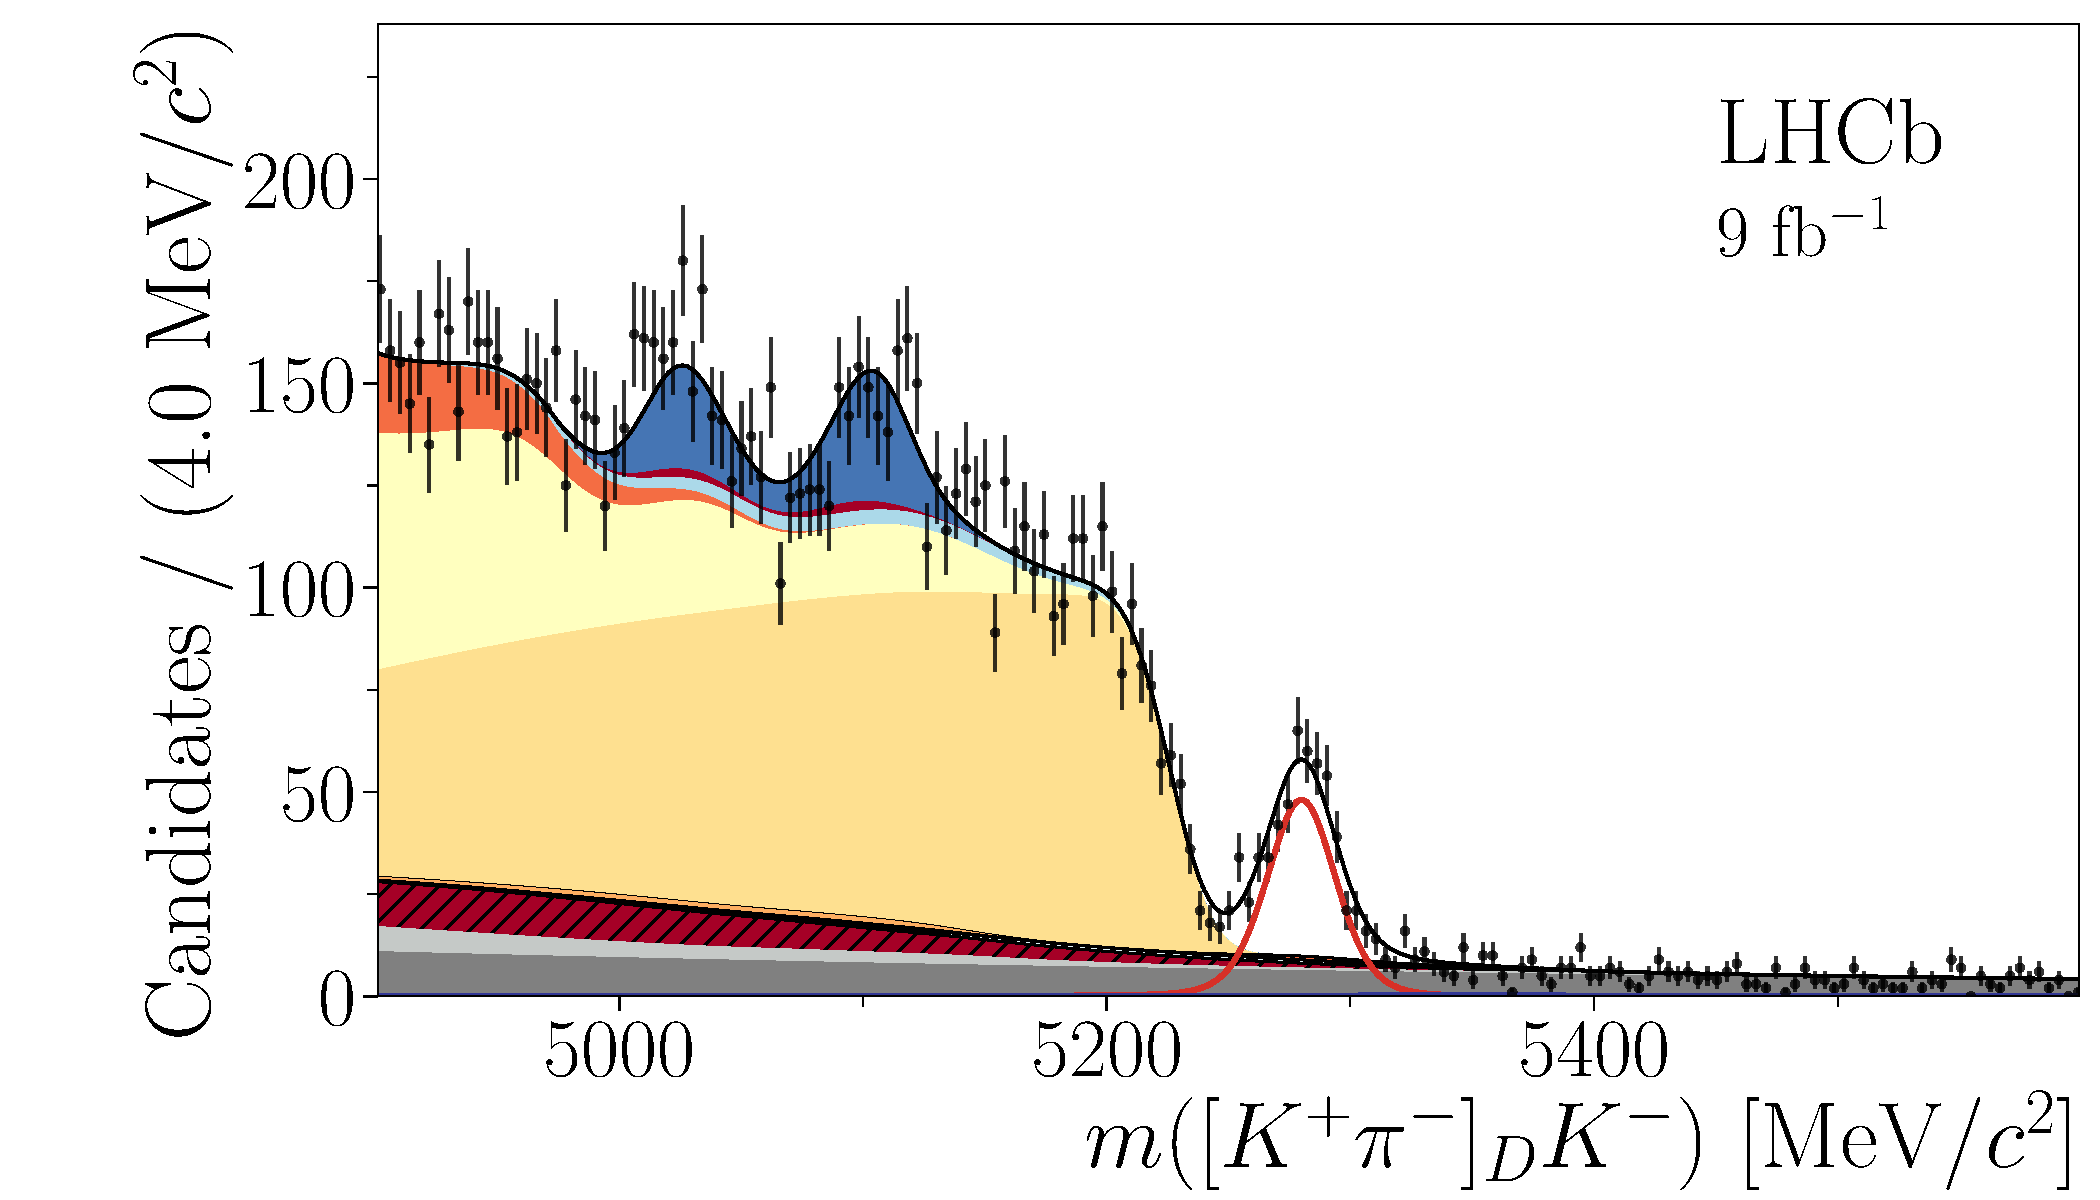
\includegraphics[width = 1.0\textwidth]{Plots/B2DK_D2Kpi_Minus.pdf}
    \end{subfigure}%
    \begin{subfigure}{0.5\textwidth}
      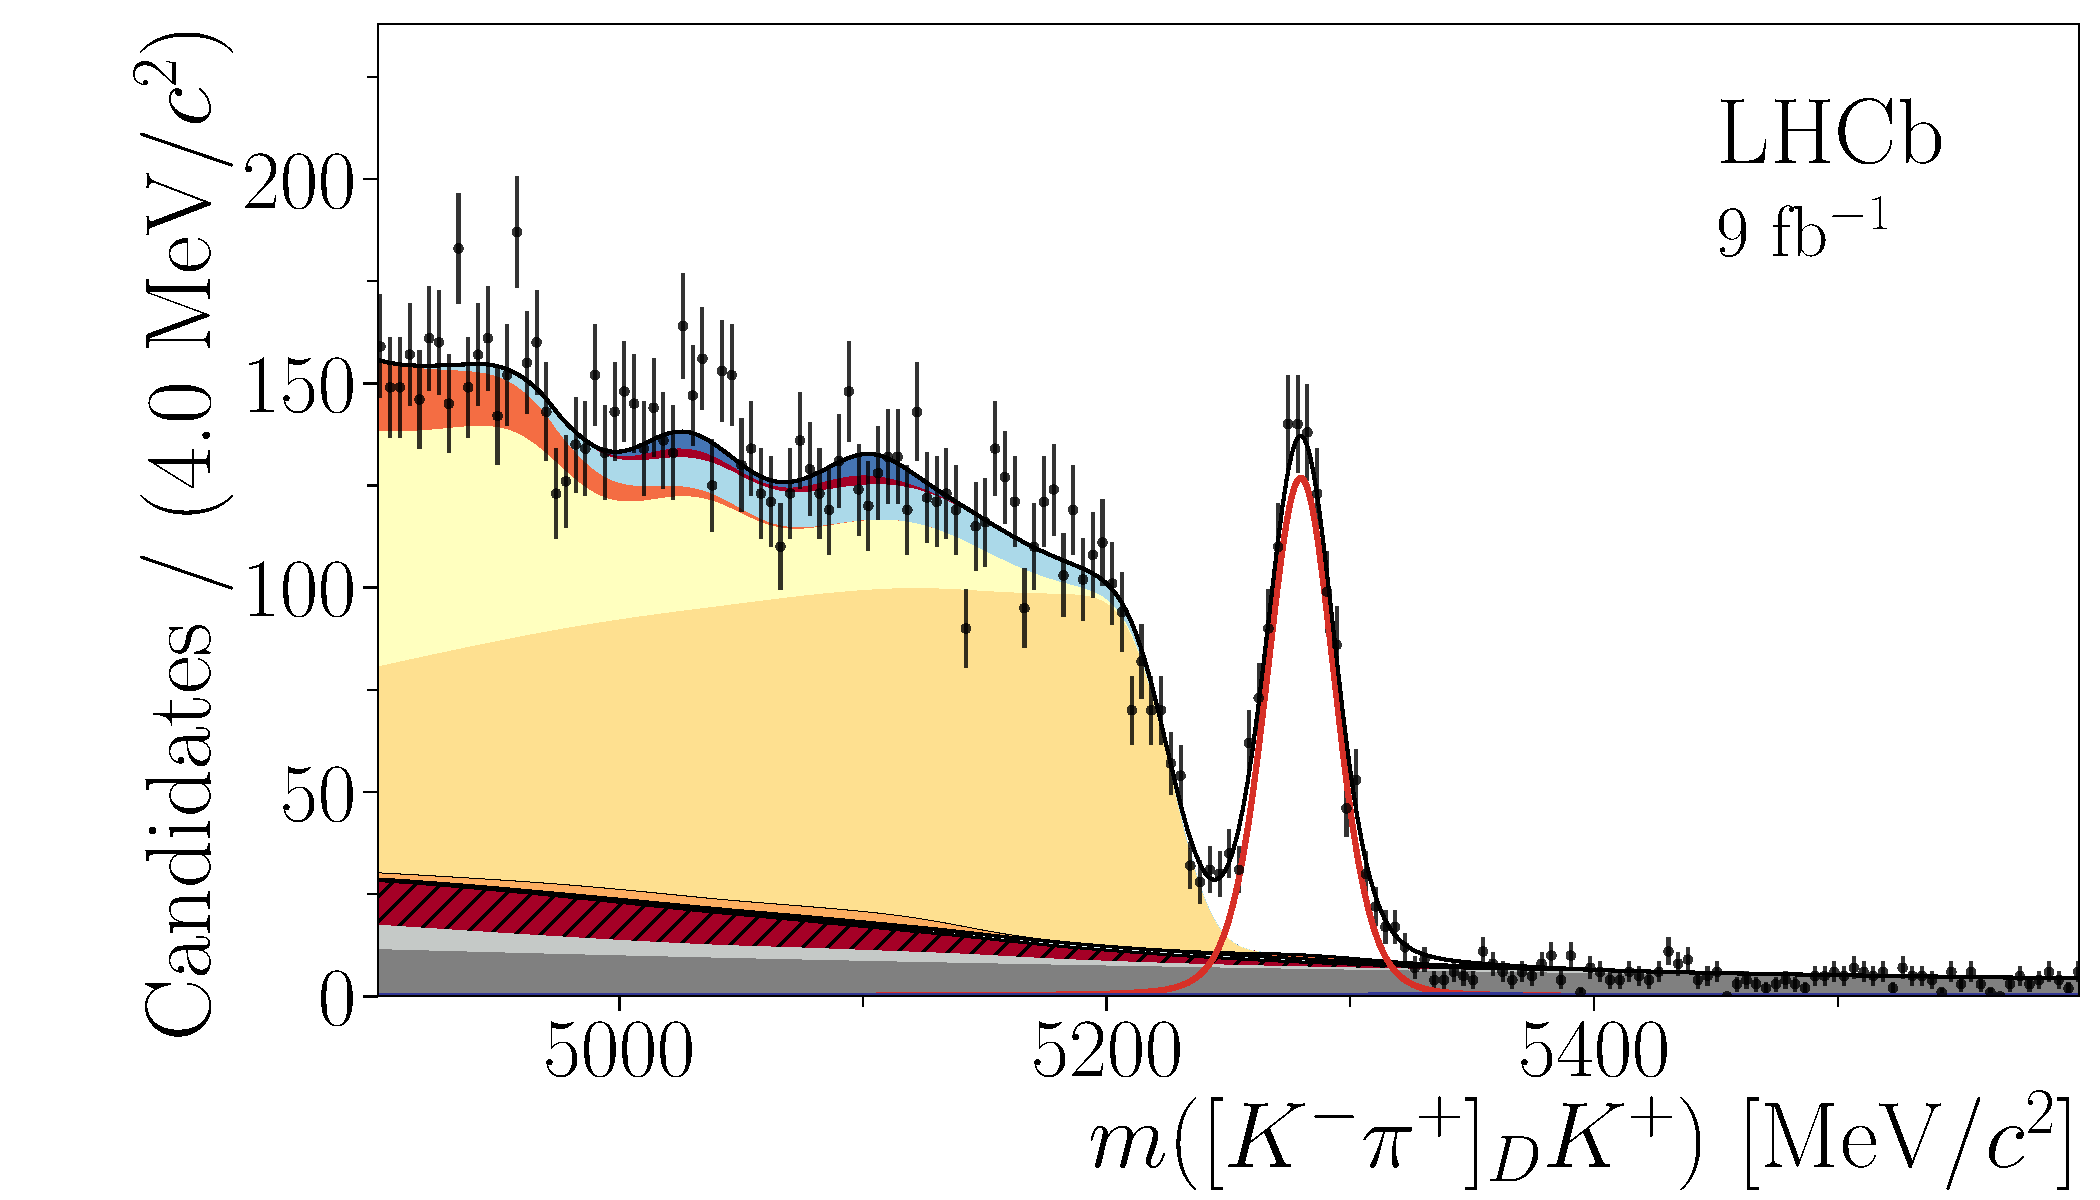
\includegraphics[width = 1.0\textwidth]{Plots/B2DK_D2Kpi_Plus.pdf}
    \end{subfigure}
    \caption*{\tiny JHEP \textbf{04} (2021) 081}
  \end{figure}
  \vspace{-0.5cm}
  \begin{center}
    \Large $B^\pm\to[K^\mp\pi^\pm]_DK^\pm$ has lower statistics, but a spectacular asymmetry!\\~\\
    \large Additionally, the partially reconstructed background has an equal but opposite asymmetry
  \end{center}
\end{frame}

\section{The \texorpdfstring{$B^\pm\to[K^+K^-\pi^+\pi^-]_DK^\pm$}{B2DKD2KKpipi} decay mode}
\begin{frame}{The $B^\pm\to[K^+K^-\pi^+\pi^-]_DK^\pm$ decay mode}
  \begin{center}
    {\huge The $B^\pm\to[K^+K^-\pi^+\pi^-]_DK^\pm$ decay mode}
  \end{center}
\end{frame}

\begin{frame}{The $B^\pm\to[K^+K^-\pi^+\pi^-]_DK^\pm$ decay mode}
  \begin{center}
    \Large The mode $B^\pm\to[K^+K^-\pi^+\pi^-]_DK^\pm$ has been proposed as a powerful channel for a measurement of $\gamma$
  \end{center}
  \begin{itemize}
    \setlength\itemsep{1.0em}
    \item{$D\to K^+K^-\pi^+\pi^-$ has the best of both worlds:}
    \begin{enumerate}
      \item{Singly Cabbibo Suppressed decay: Larger branching fraction}
      \item{Interference effects from over 25 resonance components}
    \end{enumerate}
    \item{Large interference effects in local regions of the 5D phase space}
    \item{First proposed by J. Rademacker and G. Wilkinson}
    \begin{itemize}
      \item{Phys. Lett. \textbf{B647} (2007) 400}
      \item{FOCUS amplitude model predicts a $14^\circ$ precision with $1000$ candidates}
    \end{itemize}
    \item{State of the art amplitude analysis by LHCb:}
    \begin{itemize}
      \item{JHEP \textbf{02} (2019) 126}
      \item{Exploits the huge dataset of charm decays collected by LHCb}
    \end{itemize}
  \end{itemize}
\end{frame}

\begin{frame}{The $B^\pm\to[K^+K^-\pi^+\pi^-]_DK^\pm$ decay mode}
  \begin{center}
    \Large Why do four-body decays have large local interferences?\\~\\
  \end{center}
  \begin{figure}[H]
    \centering
    \vspace{0.3cm}
    \begin{subfigure}{0.5\textwidth}
      \centering
      \begin{fmffile}{fgraph/fgraph_D2rhophi}
        \setlength{\unitlength}{0.4cm}
        \begin{fmfgraph*}(6,6)
          \fmfstraight
          \fmfleft{i1}
          \fmfv{decor.shape=circle,decor.filled=shaded,decor.size=0.2w,label=$D^0$,label.angle=180,label.dist=0.5cm}{i1}
          \fmfright{o1,o2,o3,o4}
          \fmflabel{$\pi^+$}{o1}
          \fmflabel{$\pi^-$}{o2}
          \fmflabel{$K^+$}{o3}
          \fmflabel{$K^-$}{o4}
          \fmf{plain,tension=1.5}{i1,v1}
          \fmfv{decor.shape=circle,decor.filled=shaded,decor.size=0.15w,label=\footnotesize$\phi(1020)$,label.angle=110,label.dist=1.3cm}{v1}
          \fmf{plain}{v1,o1}
          \fmf{plain}{v1,o2}
          \fmf{plain,tension=1.5}{i1,v2}
          \fmfv{decor.shape=circle,decor.filled=shaded,decor.size=0.15w,label=\footnotesize$\rho^0$,label.angle=-110,label.dist=1.2cm}{v2}
          \fmf{plain}{v2,o3}
          \fmf{plain}{v2,o4}
        \end{fmfgraph*}
      \end{fmffile}
      \vspace{0.5cm}
      \caption*{$\phi(1020)(\to K^+K^-)\rho^0(\to\pi^+\pi^-)$}
    \end{subfigure}%
    \begin{subfigure}{0.5\textwidth}
      \centering
      \begin{fmffile}{fgraph/fgraph_D2K1K}
        \setlength{\unitlength}{0.4cm}
        \begin{fmfgraph*}(6,6)
          \fmfstraight
          \fmfleft{i0,i1}
          \fmfv{decor.shape=circle,decor.filled=shaded,decor.size=0.2w,label=$D^0$,label.angle=180,label.dist=0.5cm}{i1}
          \fmfright{o1,o2,o3,o4}
          \fmflabel{$\pi^+$}{o1}
          \fmflabel{$\pi^-$}{o2}
          \fmflabel{$K^+$}{o3}
          \fmflabel{$K^-$}{o4}
          \fmf{plain,tension=2.5}{i1,v1}
          \fmfv{decor.shape=circle,decor.filled=shaded,decor.size=0.15w,label=\footnotesize$K_1(1400)^+$,label.angle=-100,label.dist=0.4cm}{v1}
          \fmf{plain}{v1,o1}
          \fmf{plain,tension=1.5}{v1,v2}
          \fmfv{decor.shape=circle,decor.filled=shaded,decor.size=0.15w,label=\footnotesize$K^*(892)^0$,label.angle=112,label.dist=0.3cm}{v2}
          \fmf{plain}{v2,o2}
          \fmf{plain}{v2,o3}          
          \fmf{plain}{i1,o4}
          \fmf{phantom,tension=3.0}{i0,v1}
        \end{fmfgraph*}
      \end{fmffile}
      \vspace{0.5cm}
      \caption*{$K_1(1400)^+(\to K^*(892)^0(\to K^+\pi^-))K^-$}
    \end{subfigure}
  \end{figure}
  \begin{center}
    \large Many possible decay paths, in different phase space locations, contribute to the total decay amplitude...
  \end{center}
\end{frame}

\begin{frame}{The $B^\pm\to[K^+K^-\pi^+\pi^-]_DK^\pm$ decay mode}
  \begin{figure}
    \centering
    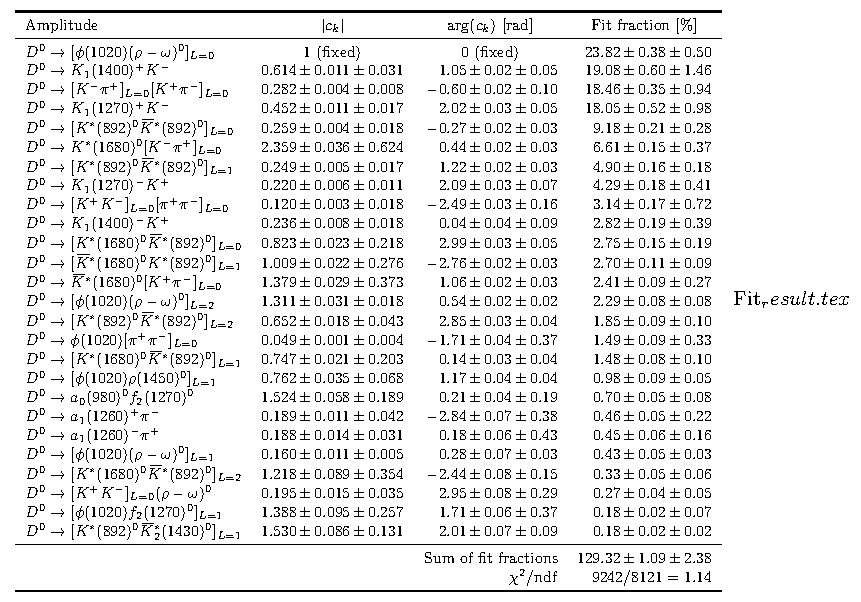
\includegraphics[width = 0.6\textwidth,trim={0 0 2.5cm 0},clip=true]{Plots/KKpipiResonances.pdf}
    \caption*{\tiny JHEP \textbf{02} (2019) 126}
  \end{figure}
  \vspace{-0.5cm}
  \begin{center}
    \Large ... and I really mean a lot of resonances!
  \end{center}
\end{frame}

\begin{frame}[fragile]{The $B^\pm\to[K^+K^-\pi^+\pi^-]_DK^\pm$ decay mode}
  \begin{center}
    Our equations suddenly become a lot more complicated\\
    \vspace{0.2cm}
    $\mathcal{A}_{D^0}(\Phi)$ now depends on a 5D phase space point $\Phi$\\
    \vspace{0.2cm}
    Defining $\mathcal{A}_{\bar{D^0}} = r_De^{i\delta_D}\mathcal{A}_{D^0}$, $r_D$ and $\delta_D$ are now also functions of $\Phi$!
  \end{center}
  \begin{equation*}
    \begin{tikzcd}[column sep=huge]
      & D^0K^- \arrow[dr, bend left = 25, "\mathcal{A}_{D^0}(\Phi)"] & \\
      B^- \arrow[ur, bend left, "\mathcal{A}_B"] \arrow[dr, bend right, "\mathcal{A}_B r_B e^{i(\delta_B - \gamma)}"'] & [5cm] & DK^- \\
      & \bar{D^0}K^- \arrow[ur, bend right = 25, "r_D(\Phi)e^{i\delta_D(\Phi)}\mathcal{A}_{D^0}(\Phi)"'] & \\
    \end{tikzcd}
  \end{equation*}
  \vspace{-0.5cm}
  \begin{equation*}
    \lvert\mathcal{A}(B^-)\lvert^2\propto1 + r_B^2r_D^2(\Phi) + 2r_Br_D(\Phi)\cos(\delta_B - \gamma + \delta_D(\Phi))
  \end{equation*}
\end{frame}

\begin{frame}{The $B^\pm\to[K^+K^-\pi^+\pi^-]_DK^\pm$ decay mode}
  \begin{center}
    \Large $r_D(\Phi)$ and $\delta_D(\Phi)$ can be predicted using the LHCb amplitude model\\~\\
    \large However, there are many reasons why we should \textbf{not} do this:
  \end{center}
  \begin{enumerate}
    \setlength\itemsep{1.0em}
    \item{$r_D(\Phi)$ can be measured directly in data at LHCb}
    \item{Amplitude models are just models, which may not reflect reality}
    \item{In fact, the model is fitted to data that knows nothing about $\delta_D(\Phi)$}
    \item{It is \underline{impossible} to assign an objective error to a model!}
  \end{enumerate}
  \begin{center}
    \large We wish to do a \underline{model independent} measurement
  \end{center}
\end{frame}

\section{Binned analysis of the \texorpdfstring{$D\to K^+K^-\pi^+\pi^-$}{D2KKpipi} mode}
\begin{frame}{Binned analysis of the $D\to K^+K^-\pi^+\pi^-$ mode}
  \begin{center}
    {\huge Binned analysis of the $D\to K^+K^-\pi^+\pi^-$ mode}
  \end{center}
\end{frame}

\begin{frame}{Binned analysis of the $D\to K^+K^-\pi^+\pi^-$ mode}
  \begin{itemize}
    \setlength\itemsep{1.0em}
    \item{Solution: Split phase space into \underline{bins}, labelled by $i = 1$, $2$, ...}
    \item{Study the CP asymmetry separately in each bin}
    \item{For the decays $D^0\to K_S^0\pi^+\pi^-$ and $K_S^0K^+K^-$, the binning scheme may be visualised on a Dalitz plot}
  \end{itemize}
  \begin{figure}
    \begin{subfigure}{0.45\textwidth}
      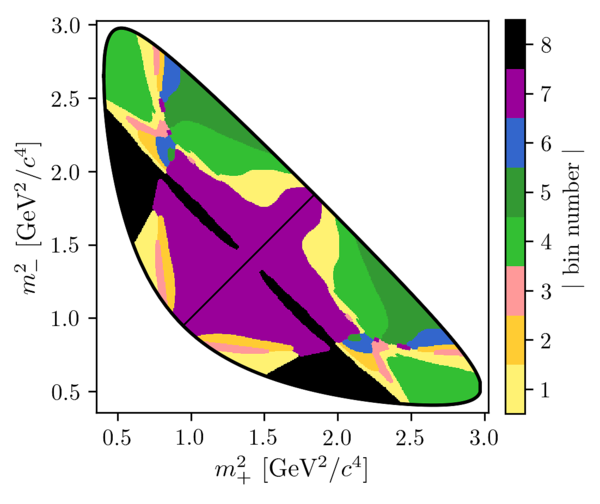
\includegraphics[height = 4cm]{Plots/KsPiPi_optimal.png}
      \caption*{$K_S^0\pi^+\pi^-$}
    \end{subfigure}%
    \begin{subfigure}{0.45\textwidth}
      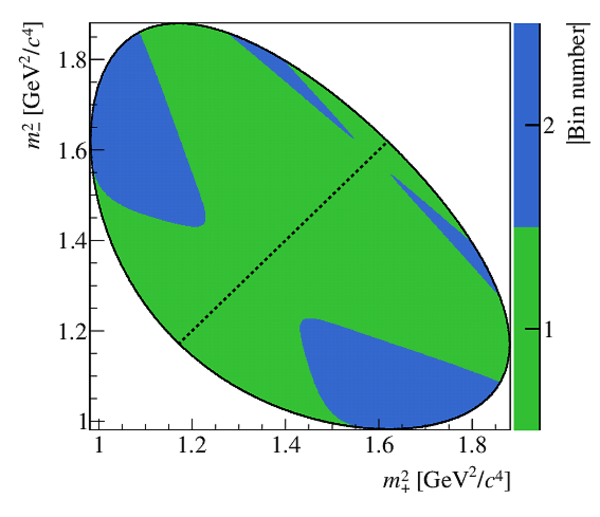
\includegraphics[height = 4cm]{Plots/KsKK_binning.png}
      \caption*{$K_S^0K^+K^-$}
    \end{subfigure}
  \end{figure}
\end{frame}

\begin{frame}{Binned analysis of the $D\to K^+K^-\pi^+\pi^-$ mode}
  \begin{figure}
    \begin{subfigure}{0.5\textwidth}
      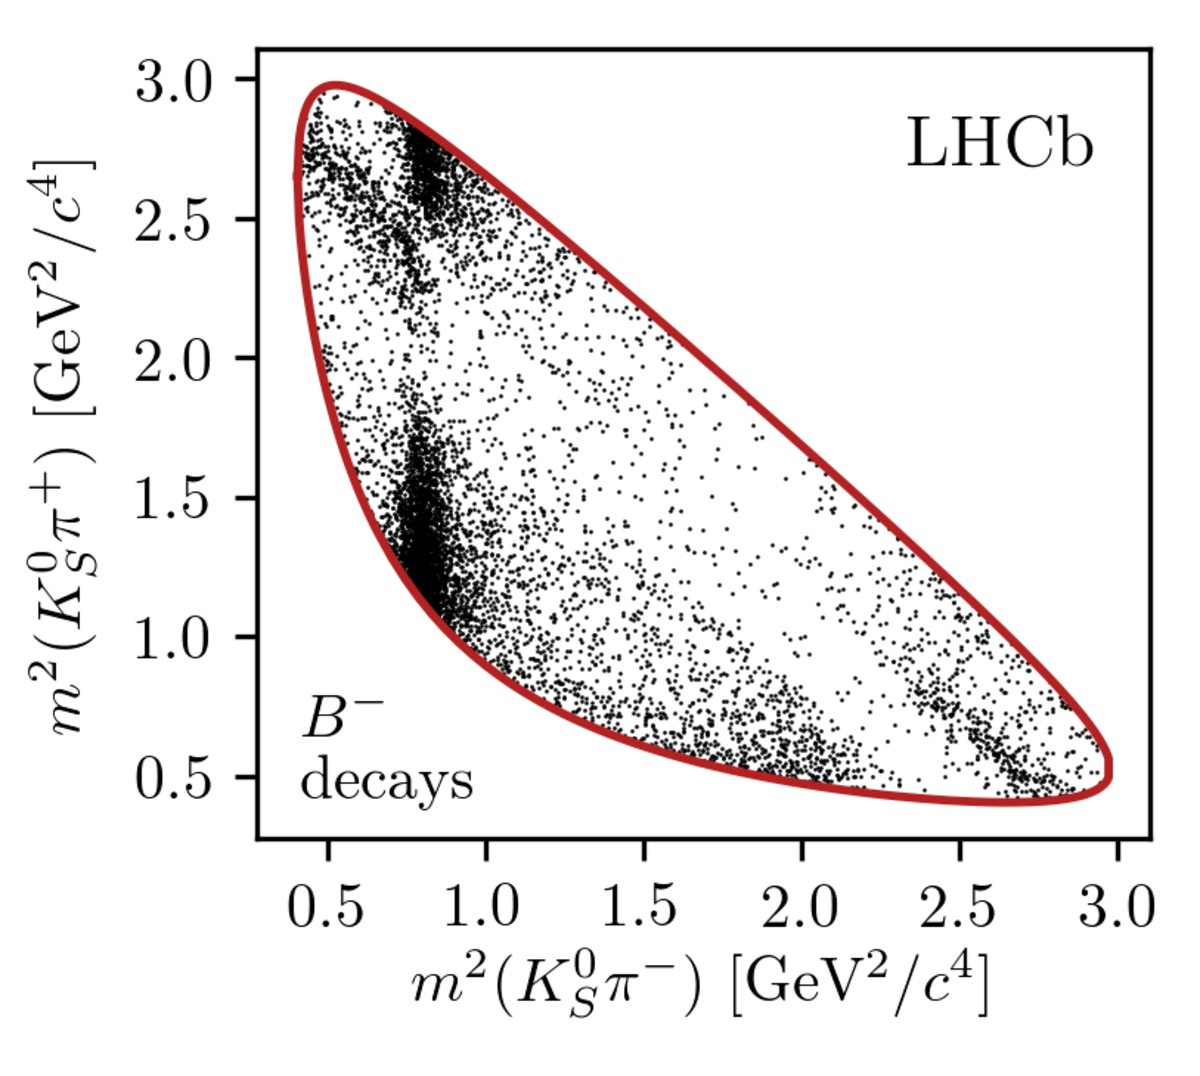
\includegraphics[width = 1.0\textwidth]{Plots/KSpipi_Minus_Dalitz.png}
      \caption*{$B^-\to[K_S^0\pi^+\pi^-]_DK^-$}
    \end{subfigure}%
    \begin{subfigure}{0.5\textwidth}
      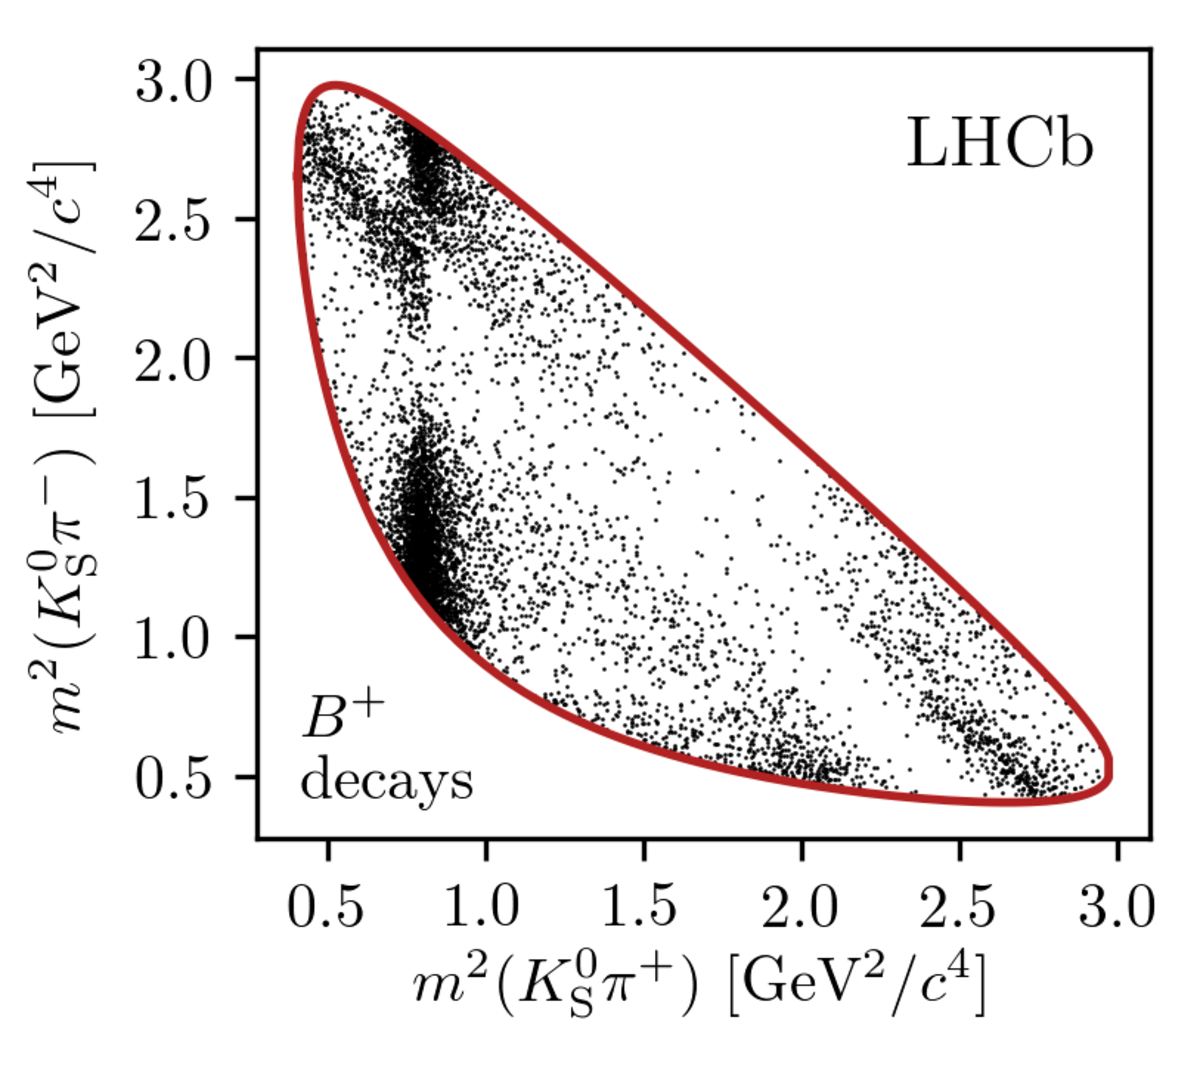
\includegraphics[width = 1.0\textwidth]{Plots/KSpipi_Plus_Dalitz.png}
      \caption*{$B^+\to[K_S^0\pi^+\pi^-]_DK^+$}
    \end{subfigure}
  \end{figure}
  \begin{center}
    \Large Can you find the asymmetries?
  \end{center}
\end{frame}

\begin{frame}{Binned analysis of the $D\to K^+K^-\pi^+\pi^-$ mode}
  \begin{center}
    \Large Back to rate equation:
  \end{center}
  \vspace{-0.3cm}
  \begin{align*}
    \lvert\mathcal{A}(B^-)\lvert^2&\propto1 + r_B^2r_D^2 \\
    &+ 2r_Br_D\big(\cos(\delta_B - \gamma)\cos(\delta_D) - \sin(\delta_B - \gamma)\sin(\delta_D)\big)
  \end{align*}
  \vspace{-0.7cm}
  \begin{center}
    \Large Integrate rate over a local region $\Phi_i$, which we call bin $i$:
  \end{center}
  \vspace{-0.3cm}
  \begin{align*}
    N_i^-&\propto F_i + r_B^2\bar{F_i} \\
    &+ 2r_B\sqrt{F_i\bar{F_i}}\big(\cos(\delta_B - \gamma)c_i - \sin(\delta_B - \gamma)s_i\big)
  \end{align*}
  \vspace{-0.7cm}
  \begin{center}
    \begin{minipage}{6cm}
      \begin{block}{\centering Amplitude averaged strong phase}
        \centering
        $c_i\equiv\frac{\int_i\mathrm{d}\Phi\lvert\mathcal{A}_{D^0}\lvert\lvert\mathcal{A}_{\bar{D^0}}\lvert\cos(\delta_D(\Phi))}{\sqrt{\int\mathrm{d}\Phi\lvert\mathcal{A}_{D^0}\lvert^2\int\mathrm{d}\Phi\lvert\mathcal{A}_{\bar{D^0}}\lvert^2}}$
      \end{block}
    \end{minipage}
  \end{center}
\end{frame}

\begin{frame}{Binned analysis of the $D\to K^+K^-\pi^+\pi^-$ mode}
  \begin{center}
    \Large To ``decouple'' the interference effects in $B^+$ and $B^-$, define the $C\!P$ violating observables
  \end{center}
  \vspace{-0.1cm}
  \begin{equation*}
    x_\pm\equiv r_B\cos(\delta_B\pm\gamma), \quad y_\pm\equiv r_B\sin(\delta_B\pm\gamma)
  \end{equation*}
  \begin{center}
    \Large Our final equation, which relates the $C\!P$ observables to experimentally measured yields, is
  \end{center}
  \begin{equation*}
    N_i^-\propto F_i + r_B^2\bar{F_i} + 2\sqrt{F_i\bar{F_i}}\big(x_-c_i - y_-s_i\big)
  \end{equation*}
  \vspace{-0.7cm}
  \begin{center}
    \begin{minipage}{6cm}
      \begin{block}{\centering Amplitude averaged strong phase}
        \centering
        $c_i\equiv\frac{\int_i\mathrm{d}\Phi\lvert\mathcal{A}_{D^0}\lvert\lvert\mathcal{A}_{\bar{D^0}}\lvert\cos(\delta_D(\Phi))}{\sqrt{\int\mathrm{d}\Phi\lvert\mathcal{A}_{D^0}\lvert^2\int\mathrm{d}\Phi\lvert\mathcal{A}_{\bar{D^0}}\lvert^2}}$
      \end{block}
    \end{minipage}
  \end{center}
\end{frame}

\begin{frame}{Binned analysis of the $D\to K^+K^-\pi^+\pi^-$ mode}
  \begin{center}
    \begin{minipage}{8cm}
      \begin{block}{\centering Bin yield}
        \vspace{-0.5cm}
        \begin{equation*}
          N_i^-\propto F_i + r_B^2\bar{F_i} + 2\sqrt{F_i\bar{F_i}}\big(x_-c_i - y_-s_i\big)
        \end{equation*}
      \end{block}
    \end{minipage}
  \end{center}
  \vspace{0.3cm}
  \begin{center}
    \Large The strategy for measuring $\gamma$ is now clear:
  \end{center}
  \begin{enumerate}
    \setlength\itemsep{1.0em}
    \item{Measure bin yields $N_i^\pm$ in $B^\pm\to[K^+K^-\pi^+\pi^-]_DK^\pm$ decays}
    \item{Do a likelihood maximisation to determine $F_i$, $\bar{F_i}$, $c_i$, $s_i$, $x_\pm$ and $y_\pm$}
    \item{From $x_\pm$ and $y_\pm$, extract $r_B$, $\delta_B$ and $\gamma$}
    \item{Publish new measurement of $\gamma$!}
  \end{enumerate}
\end{frame}

\section{Strong phase input from charm factories}
\begin{frame}{Strong phase input from charm factories}
  \begin{center}
    {\huge Strong phase input from charm factories}
  \end{center}
\end{frame}

\begin{frame}{Strong phase input from charm factories}
  \begin{center}
    \Large Unfortunately, it is unlikely that this fit will converge... \\
    \large Sensitivity to $c_i$ and $s_i$ is very limited with current statistics
  \end{center}
  \begin{center}
    \phantom{Instead, we can join forces with BESIII}
  \end{center}
  \begin{figure}
    \begin{subfigure}{0.5\textwidth}
      \phantom{
\includegraphics[height = 2cm]{lhcb.jpg}}
    \end{subfigure}%
    \begin{subfigure}{0.5\textwidth}
      \phantom{
\includegraphics[height = 2cm]{bes3.jpg}}
    \end{subfigure}
  \end{figure}
  \vspace{0.3cm}
  \begin{center}
    \phantom{\large This has never been done for $D^0\to K^+K^-\pi^+\pi^-$}\\
    \phantom{\large More on this later!}
  \end{center}
\end{frame}

\begin{frame}{Strong phase input from charm factories}
  \begin{center}
    \Large Unfortunately, it is unlikely that this fit will converge... \\
    \large Sensitivity to $c_i$ and $s_i$ is very limited with current statistics
  \end{center}
  \begin{center}
    Instead, we can join forces with BESIII and measure $c_i$ and $s_i$ directly
  \end{center}
  \begin{figure}
    \centering
    \begin{subfigure}{0.35\textwidth}
      \centering
      
\includegraphics[height = 2cm]{lhcb.jpg}
    \end{subfigure}%
    {\Huge $+$}
    \begin{subfigure}{0.45\textwidth}
      \centering
      
\includegraphics[height = 2cm]{bes3.jpg}
    \end{subfigure}
  \end{figure}
  \vspace{0.3cm}
  \begin{center}
    \large This has never been done for $D^0\to K^+K^-\pi^+\pi^-$\\
    \large More on this later!
  \end{center}
\end{frame}

\section{Constraining \texorpdfstring{$F_i$}{Fi} with \texorpdfstring{$B^\pm\to D\pi^\pm$}{B2Dpi}}
\begin{frame}{Constraining $F_i$ with $B^\pm\to D\pi^\pm$}
  \begin{center}
    {\huge Constraining $F_i$ with $B^\pm\to D\pi^\pm$}
  \end{center}
\end{frame}

\begin{frame}{Constraining $F_i$ with $B^\pm\to D\pi^\pm$}
  \begin{itemize}
    \setlength\itemsep{1.0em}
    \item{The fractional bin yields $F_i$ are yields in the abscence of $C\!P$ violation}
    \item{In principle we can measure these directly at both LHCb and BESIII}
  \end{itemize}
  \begin{center}
    Four strategies:
  \end{center}
  \begin{enumerate}
    \setlength\itemsep{1.0em}
    \item{Calculate from amplitude model}
    \item{Measure in $B^-\to D^0\mu^-\bar{\nu_\mu}$ at LHCb}
    \item{Measure with flavour tagged $D^0$ decays at BESIII}
    \item{Measure in $B^\pm\to D\pi^\pm$}
  \end{enumerate}
  \vspace{0.1cm}
  \begin{center}
    \phantom{No problem, include $B^\pm\to D\pi^\pm$ as a \underline{signal channel}}
  \end{center}
\end{frame}

\begin{frame}{Constraining $F_i$ with $B^\pm\to D\pi^\pm$}
  \begin{itemize}
    \setlength\itemsep{1.0em}
    \item{The fractional bin yields $F_i$ are yields in the abscence of $C\!P$ violation}
    \item{In principle we can measure these directly at both LHCb and BESIII}
  \end{itemize}
  \begin{center}
    Four strategies:
  \end{center}
  \begin{enumerate}
    \setlength\itemsep{1.0em}
    \item{\sout{Calculate from amplitude model}\quad Avoid model dependence}
    \item{Measure in $B^-\to D^0\mu^-\bar{\nu_\mu}$ at LHCb}
    \item{Measure with flavour tagged $D^0$ decays at BESIII}
    \item{Measure in $B^\pm\to D\pi^\pm$}
  \end{enumerate}
  \vspace{0.1cm}
  \begin{center}
    \phantom{No problem, include $B^\pm\to D\pi^\pm$ as a \underline{signal channel}}
  \end{center}
\end{frame}

\begin{frame}{Constraining $F_i$ with $B^\pm\to D\pi^\pm$}
  \begin{itemize}
    \setlength\itemsep{1.0em}
    \item{The fractional bin yields $F_i$ are yields in the abscence of $C\!P$ violation}
    \item{In principle we can measure these directly at both LHCb and BESIII}
  \end{itemize}
  \begin{center}
    Four strategies:
  \end{center}
  \begin{enumerate}
    \setlength\itemsep{1.0em}
    \item{\sout{Calculate from amplitude model}\quad Avoid model dependence}
    \item{\sout{Measure in $B^-\to D^0\mu^-\bar{\nu_\mu}$ at LHCb}\quad Different acceptance effects}
    \item{\sout{Measure with flavour tagged $D^0$ decays at BESIII}}
    \item{Measure in $B^\pm\to D\pi^\pm$}
  \end{enumerate}
  \vspace{0.1cm}
  \begin{center}
    \phantom{No problem, include $B^\pm\to D\pi^\pm$ as a \underline{signal channel}}
  \end{center}
\end{frame}

\begin{frame}{Constraining $F_i$ with $B^\pm\to D\pi^\pm$}
  \begin{itemize}
    \setlength\itemsep{1.0em}
    \item{The fractional bin yields $F_i$ are yields in the abscence of $C\!P$ violation}
    \item{In principle we can measure these directly at both LHCb and BESIII}
  \end{itemize}
  \begin{center}
    Four strategies:
  \end{center}
  \begin{enumerate}
    \setlength\itemsep{1.0em}
    \item{\sout{Calculate from amplitude model}\quad Avoid model dependence}
    \item{\sout{Measure in $B^-\to D^0\mu^-\bar{\nu_\mu}$ at LHCb}\quad Different acceptance effects}
    \item{\sout{Measure with flavour tagged $D^0$ decays at BESIII}}
    \item{\underline{Measure in $B^\pm\to D\pi^\pm$}\quad Small CPV effects?}
  \end{enumerate}
  \vspace{0.1cm}
  \begin{center}
    \phantom{No problem, include $B^\pm\to D\pi^\pm$ as a \underline{signal channel}}
  \end{center}
\end{frame}

\begin{frame}{Constraining $F_i$ with $B^\pm\to D\pi^\pm$}
  \begin{itemize}
    \setlength\itemsep{1.0em}
    \item{The fractional bin yields $F_i$ are yields in the abscence of $C\!P$ violation}
    \item{In principle we can measure these directly at both LHCb and BESIII}
  \end{itemize}
  \begin{center}
    Four strategies:
  \end{center}
  \begin{enumerate}
    \setlength\itemsep{1.0em}
    \item{\sout{Calculate from amplitude model}\quad Avoid model dependence}
    \item{\sout{Measure in $B^-\to D^0\mu^-\bar{\nu_\mu}$ at LHCb}\quad Different acceptance effects}
    \item{\sout{Measure with flavour tagged $D^0$ decays at BESIII}}
    \item{\underline{Measure in $B^\pm\to D\pi^\pm$}\quad Small CPV effects?}
  \end{enumerate}
  \vspace{0.1cm}
  \begin{center}
    No problem, include $B^\pm\to D\pi^\pm$ as a \underline{signal channel}
  \end{center}
\end{frame}

\begin{frame}{Constraining $F_i$ with $B^\pm\to D\pi^\pm$}
  \begin{itemize}
    \setlength\itemsep{1.5em}
    \item{$B^\pm\to D\pi^\pm$ has an identical topology to $B^\pm\to DK^\pm$}
    \item{CPV effects are highly suppressed because $r_B^{D\pi}\approx0.005$}
    \item{Branching fraction more than 10 times larger}
    \item{As a signal channel, we add another 4 free parameters to our fit:}
  \end{itemize}
  \begin{equation*}
    x_\pm^{D\pi} = r_B^{D\pi}\cos(\delta_B^{D\pi} - \gamma),\quad y_\pm^{D\pi} = r_B^{D\pi}\sin(\delta_B^{D\pi} - \gamma)
  \end{equation*}
\end{frame}

\begin{frame}{Constraining $F_i$ with $B^\pm\to D\pi^\pm$}
  \begin{center}
    To avoid degeneracy, reduce this to 2 additional parameters using this parameterisation:
  \end{center}
  \begin{equation*}
    x_\xi = \Re(\xi),\quad y_\xi = \Im(\xi),\quad \xi = \frac{r_B^{D\pi}e^{i\delta_B^{D\pi}}}{r_B^{DK}e^{i\delta_B^{DK}}}
  \end{equation*}
  \begin{center}
    In summary:
  \end{center}
  \begin{enumerate}
    \setlength\itemsep{1.0em}
    \item{Both $B^\pm\to DK^\pm$ and $B^\pm\to D\pi^\pm$ are signal channels, with $x_\pm^{DK}$, $y_\pm^{DK}$, $x_\xi$ and $y_\xi$ as $C\!P$ observables}
    \item{$B^\pm\to DK^\pm$ has lower statistics, but higher CPV effects}
    \item{$B^\pm\to D\pi^\pm$ has higher statistics and constrain $F_i$ in the fit, but sensitivity to CPV is limited}
  \end{enumerate}
\end{frame}

\section{Binning scheme}
\begin{frame}{Binning scheme}
  \begin{center}
    {\huge Binning scheme}
  \end{center}
\end{frame}

\begin{frame}{Binning scheme}
  \begin{center}
    \Large We need to split the phase space into bins\\~\\
    \large But how do we navigate through a 5D space? How do we decide on the bin boundaries?
  \end{center}
  \vspace{-0.5cm}
  \begin{figure}
    \centering
    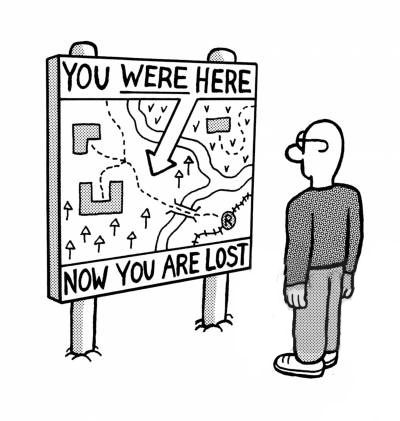
\includegraphics[width = 0.35\textwidth]{Plots/TravelLost.jpeg}
  \end{figure}
  \vspace{-0.7cm}
  \begin{center}
    \Large Let the amplitude model guide us!
  \end{center}
\end{frame}

\begin{frame}{Binning scheme}
  \vspace{0.0cm}
  {\large Back to the amplitude averaged strong phase:}
  \begin{equation*}
    c_i\equiv\frac{\int_i\mathrm{d}\Phi\lvert\mathcal{A}_{D^0}\lvert\lvert\mathcal{A}_{\bar{D^0}}\lvert\cos(\delta_D(\Phi))}{\sqrt{\int\mathrm{d}\Phi\lvert\mathcal{A}_{D^0}\lvert^2\int\mathrm{d}\Phi\lvert\mathcal{A}_{\bar{D^0}}\lvert^2}}
  \end{equation*}
  \begin{itemize}
    \setlength\itemsep{0.5em}
    \item{If the strong phase varies significantly within a bin, the interference effects will be diluted when integrating}
    \item{We need to group regions of similar strong phase into the same bin}
    \item{This was done for $K_S^0h^+h^-$, resulting in colourful ``butterfly'' plots}
  \end{itemize}
  \begin{figure}
    \centering
    \begin{subfigure}{0.45\textwidth}
      \centering
      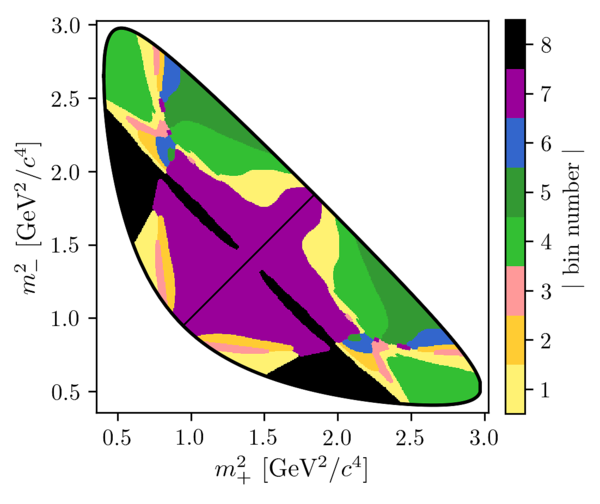
\includegraphics[height = 3cm]{Plots/KsPiPi_optimal.png}
    \end{subfigure}%
    \begin{subfigure}{0.45\textwidth}
      \centering
      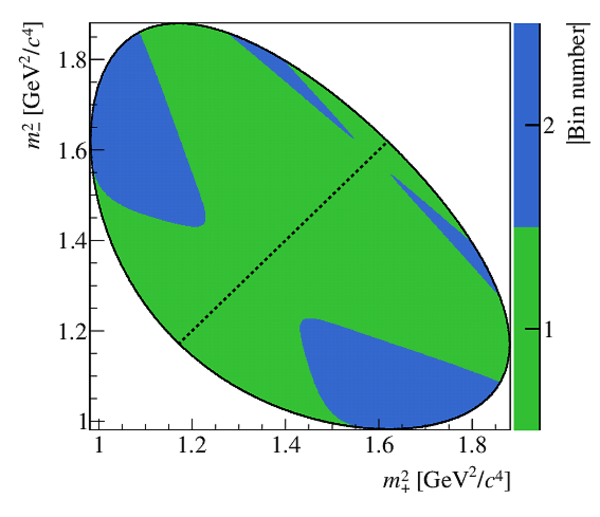
\includegraphics[height = 3cm]{Plots/KsKK_binning.png}
    \end{subfigure}
  \end{figure}
\end{frame}

\begin{frame}{Binning scheme}
  \vspace{0.0cm}
  {\large Back to our yield formula:}
  \begin{equation*}
    N_i^-\propto F_i + r_B^2\bar{F_i} + 2\sqrt{F_i\bar{F_i}}\big(x_-c_i - y_-s_i\big)
  \end{equation*}
  \vspace{-0.3cm}
  \begin{itemize}
    \setlength\itemsep{0.5em}
    \item{In the charm system, $C\!P$ is (approximately) conserved, so each $D^0$ decay has a corresponding identical $C\!P$ conjugated decay}
    \item{Split each bin $i$ into two ``$C\!P$ mirror bins'', labelled by $\pm i$}
    \item{In $K_S^0h^+h^-$, this is indicated by the black symmetry line}
    \item{Under $C\!P$, $\delta_D\to-\delta_D$, so $c_i\to c_i$ and $s_i\to -s_i$}
  \end{itemize}
  \begin{figure}
    \centering
    \begin{subfigure}{0.45\textwidth}
      \centering
      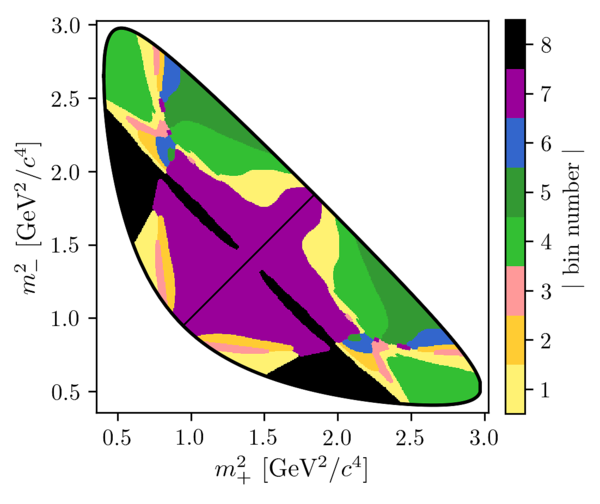
\includegraphics[height = 3cm]{Plots/KsPiPi_optimal.png}
    \end{subfigure}%
    \begin{subfigure}{0.45\textwidth}
      \centering
      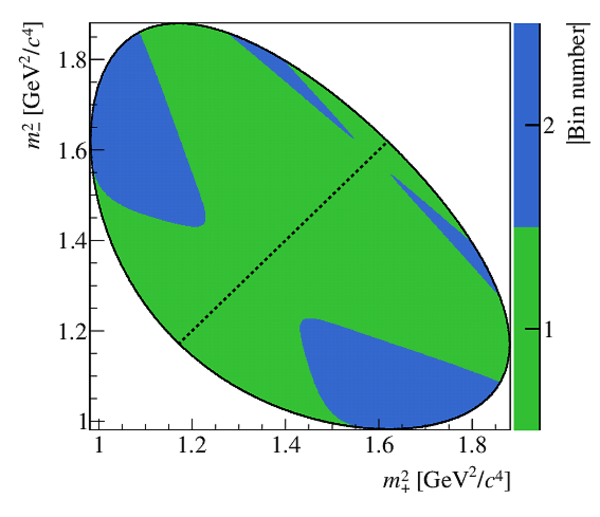
\includegraphics[height = 3cm]{Plots/KsKK_binning.png}
    \end{subfigure}
  \end{figure}
\end{frame}

\begin{frame}{Binning scheme}
  \vspace{0.0cm}
  {\Large A binning scheme must satisfy the following:}
  \begin{itemize}
    \item{Minimal dilution of strong phases when integrating over bins}
    \item{Enhance interference between $B^\pm\to D^0K^\pm$ and $B^\pm\to\bar{D^0}K^\pm$}
  \end{itemize}
  \vspace{0.4cm}
  {\Large How to bin a 5-dimensional phase space?}
  \begin{enumerate}
    \item{For each $B^\pm$ candidate, use the amplitude model to calculate}
  \end{enumerate}
  \begin{center}
    {\Large $\frac{\mathcal{A}(D^0)}{\mathcal{A}(\bar{D^0})} = r_De^{i\delta_D}$}
  \end{center}
  \begin{enumerate}
    \setcounter{enumi}{1}
    \setlength\itemsep{0.5em}
    \item{Split $\delta_D$ into uniformly spaced bins}
    \item{Use the symmetry line $r_D = 1$ to separate bin $+i$ from $-i$}
    \item{Optimise the binning scheme by adjusting the bin boundaries in $\delta_D$}
  \end{enumerate}
\end{frame}

\begin{frame}{Binning scheme}
  \begin{figure}
    \centering
    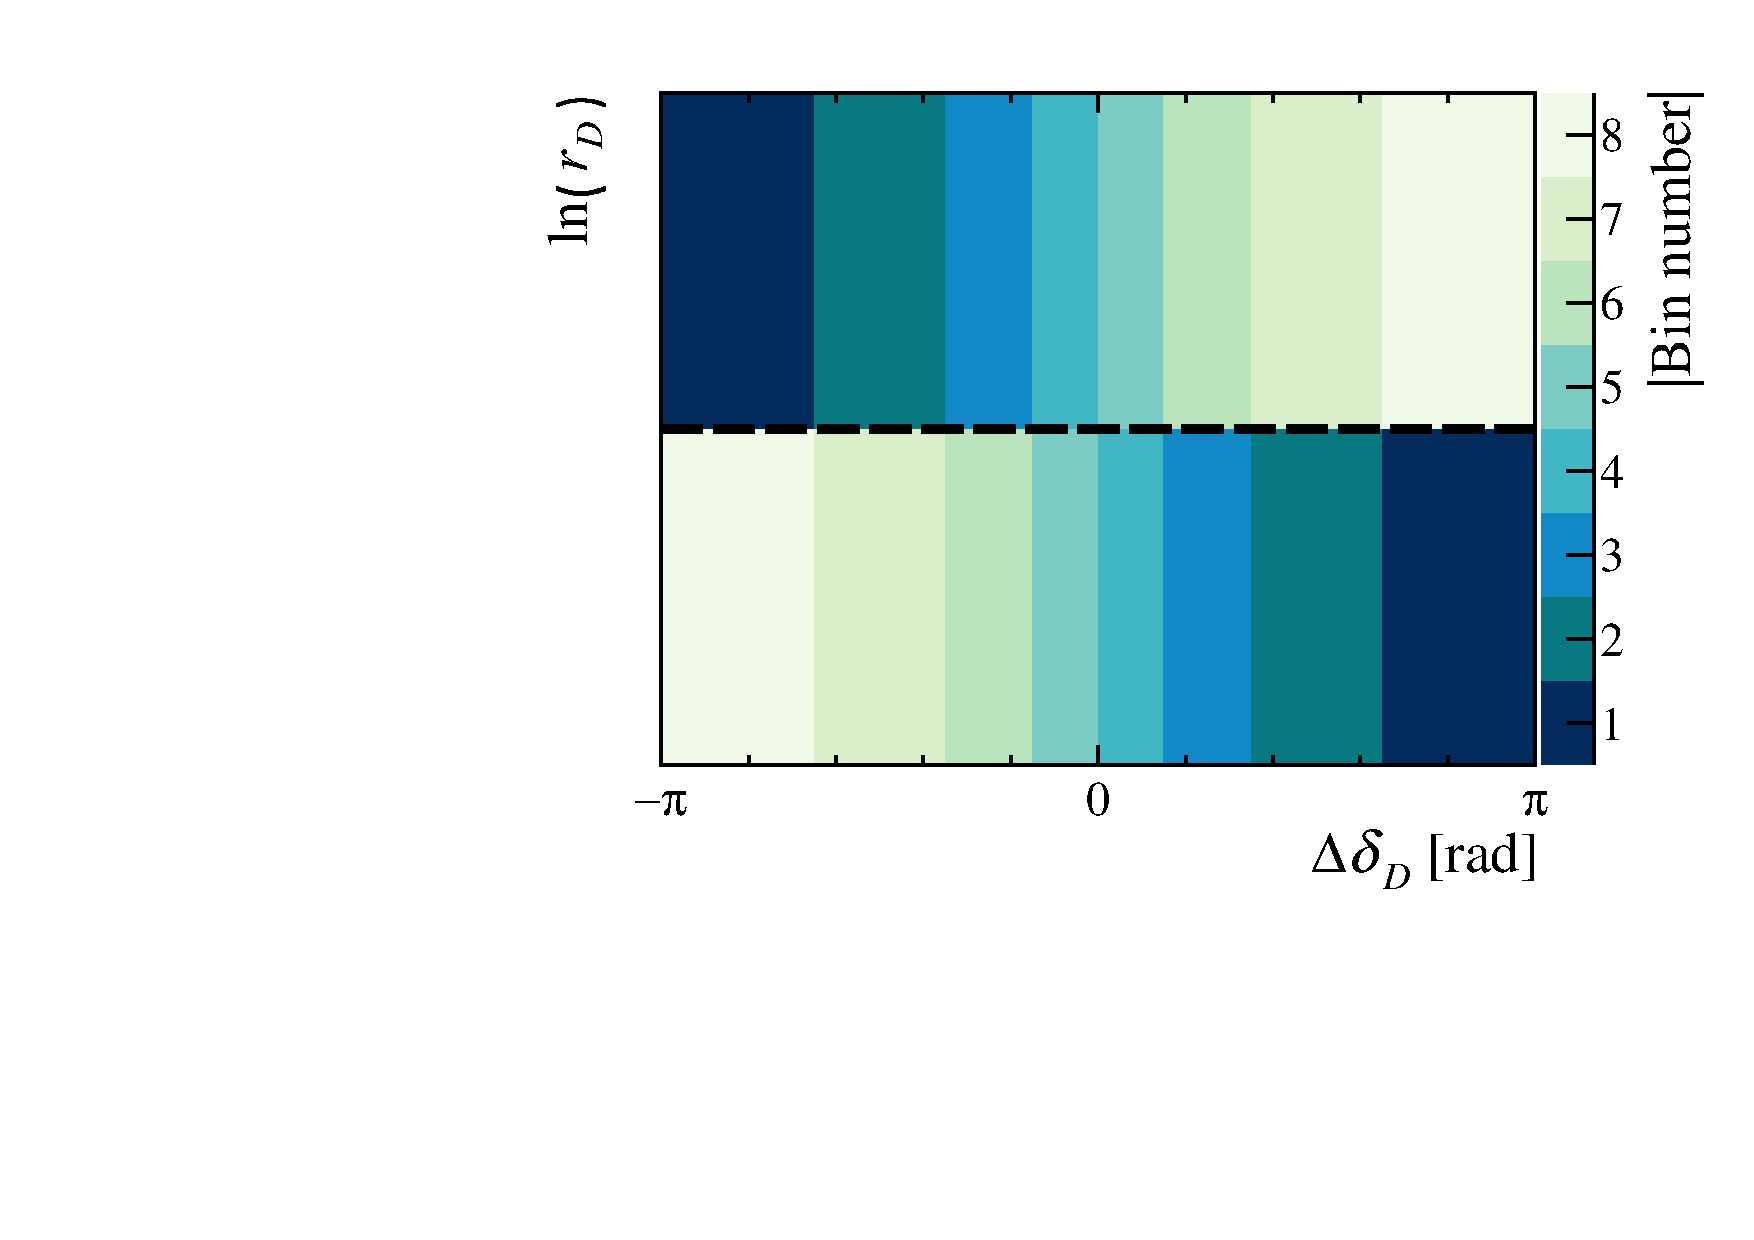
\includegraphics[width = 0.7\textwidth]{Plots/BinningSchemePlot_8Bins.pdf}
  \end{figure}
  \vspace{-1.0cm}
  \begin{center}
    $Q = 0.90$ \\
    Bins $i < 0$ on top, $i > 0$ below
  \end{center}
\end{frame}

\section{Mass fits and yield extraction}
\begin{frame}{Mass fits and yield extraction}
  \begin{center}
    {\huge Mass fits and yield extraction}
  \end{center}
\end{frame}

\begin{frame}{Mass fits and yield extraction}
  \begin{center}
    \large In the end, this analysis is a counting experiment
  \end{center}
  Counting strategy:
  \begin{enumerate}
    \setlength\itemsep{1.0em}
    \item{Perform a ``global fit'' of all $B^\pm$ candidates}
    \item{Fix all shape parameters}
    \item{Sort $B^\pm$ candidates by charge and bins}
    \item{Perform a ``$C\!P$ fit'' simultaneously, but only let bin yields float}
    \item{From the bin yields, determine $x_\pm^{DK}$, $y_\pm^{DK}$, $x_\xi$ and $y_\xi$}
  \end{enumerate}
\end{frame}

\begin{frame}{Mass fits and yield extraction}
  \begin{figure}
    \centering
    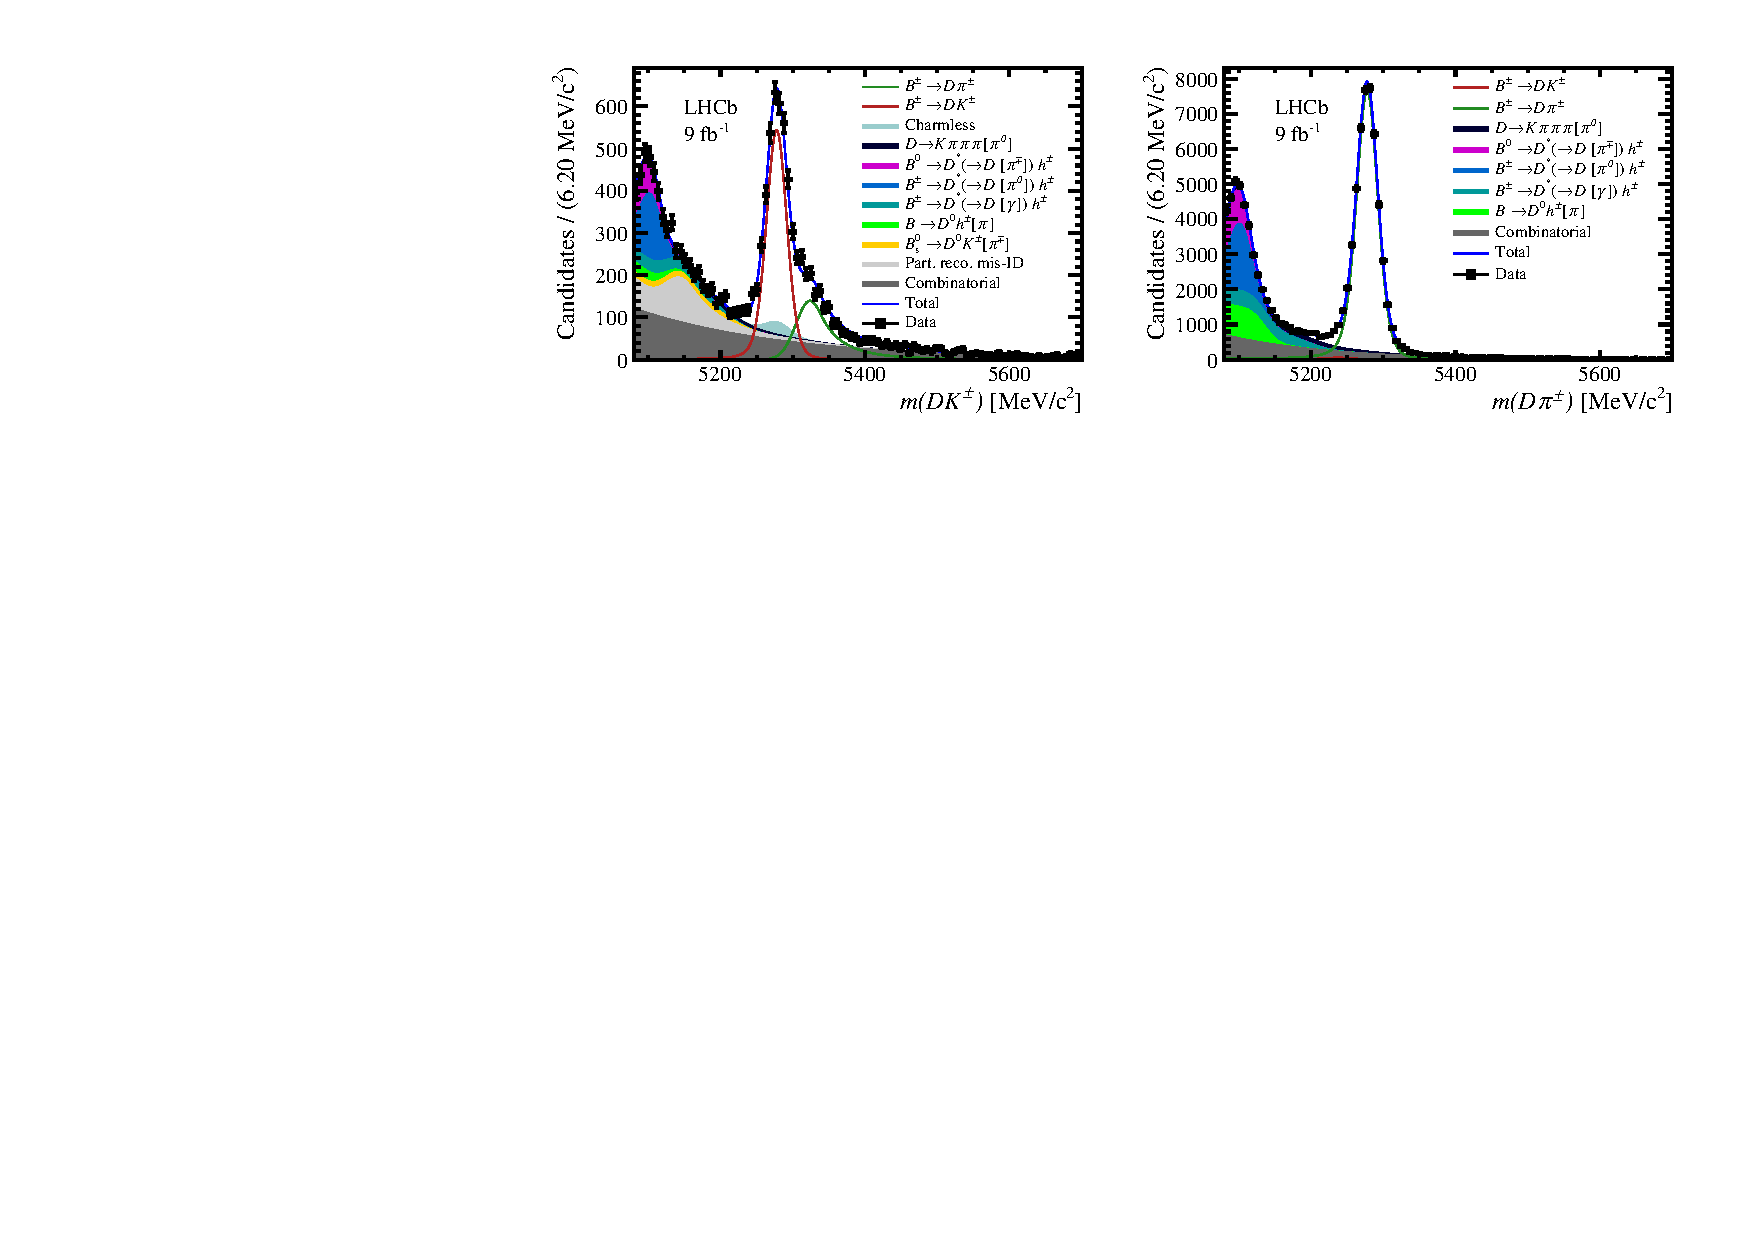
\includegraphics[width = 1.0\textwidth]{Plots/d2kkpipi_fiveL_allDP.pdf}
  \end{figure}
  \begin{center}
    Signal yield:
  \end{center}
  \vspace{-0.3cm}
  \begin{align*}
    B^\pm\to DK^\pm:&\quad \SI{3026(38)}{} \\
    B^\pm\to D\pi^\pm:&\quad \SI{44349(218)}{}
  \end{align*}
\end{frame}

\begin{frame}{Mass fits and yield extraction}
  \begin{center}
    \Large $C\!P$ fit setup
  \end{center}
  \begin{itemize}
    \setlength\itemsep{0.5em}
    \item{No measurement of $c_i$ and $s_i$ available yet, use model predictions}
    \item{Fix mass shape from global fit}
    \item{Split by $B^\pm$ charge and $D$ phase space bins ($64$ categories)}
  \end{itemize}
  \vspace{0.3cm}
  \begin{enumerate}
    \setlength\itemsep{0.5em}
    \item{CP observables $x_\pm^{DK}$, $y_\pm^{DK}$ $x_\xi^{D\pi}$, $y_\xi^{D\pi}$ ($6$ parameters
)}
    \item{Fractional bin yields $F_i$ ($15$ parameters)}
    \item{Low mass and combinatorial background ($128$ parameters)}
    \item{Yield normalisation ($4$ parameters)}
  \end{enumerate}
  In total: 153 free parameters
\end{frame}

\section{\texorpdfstring{$C\!P$}{CP} fit results and \texorpdfstring{$\gamma$}{gamma}}
\begin{frame}{$C\!P$ fit results and $\gamma$}
  \begin{center}
    {\huge $C\!P$ fit results and $\gamma$}
  \end{center}
\end{frame}

\begin{frame}{Fractional bin asymmetries}
  \begin{figure}
    \centering
    \vspace{-0.2cm}
    \begin{subfigure}{0.5\textwidth}
      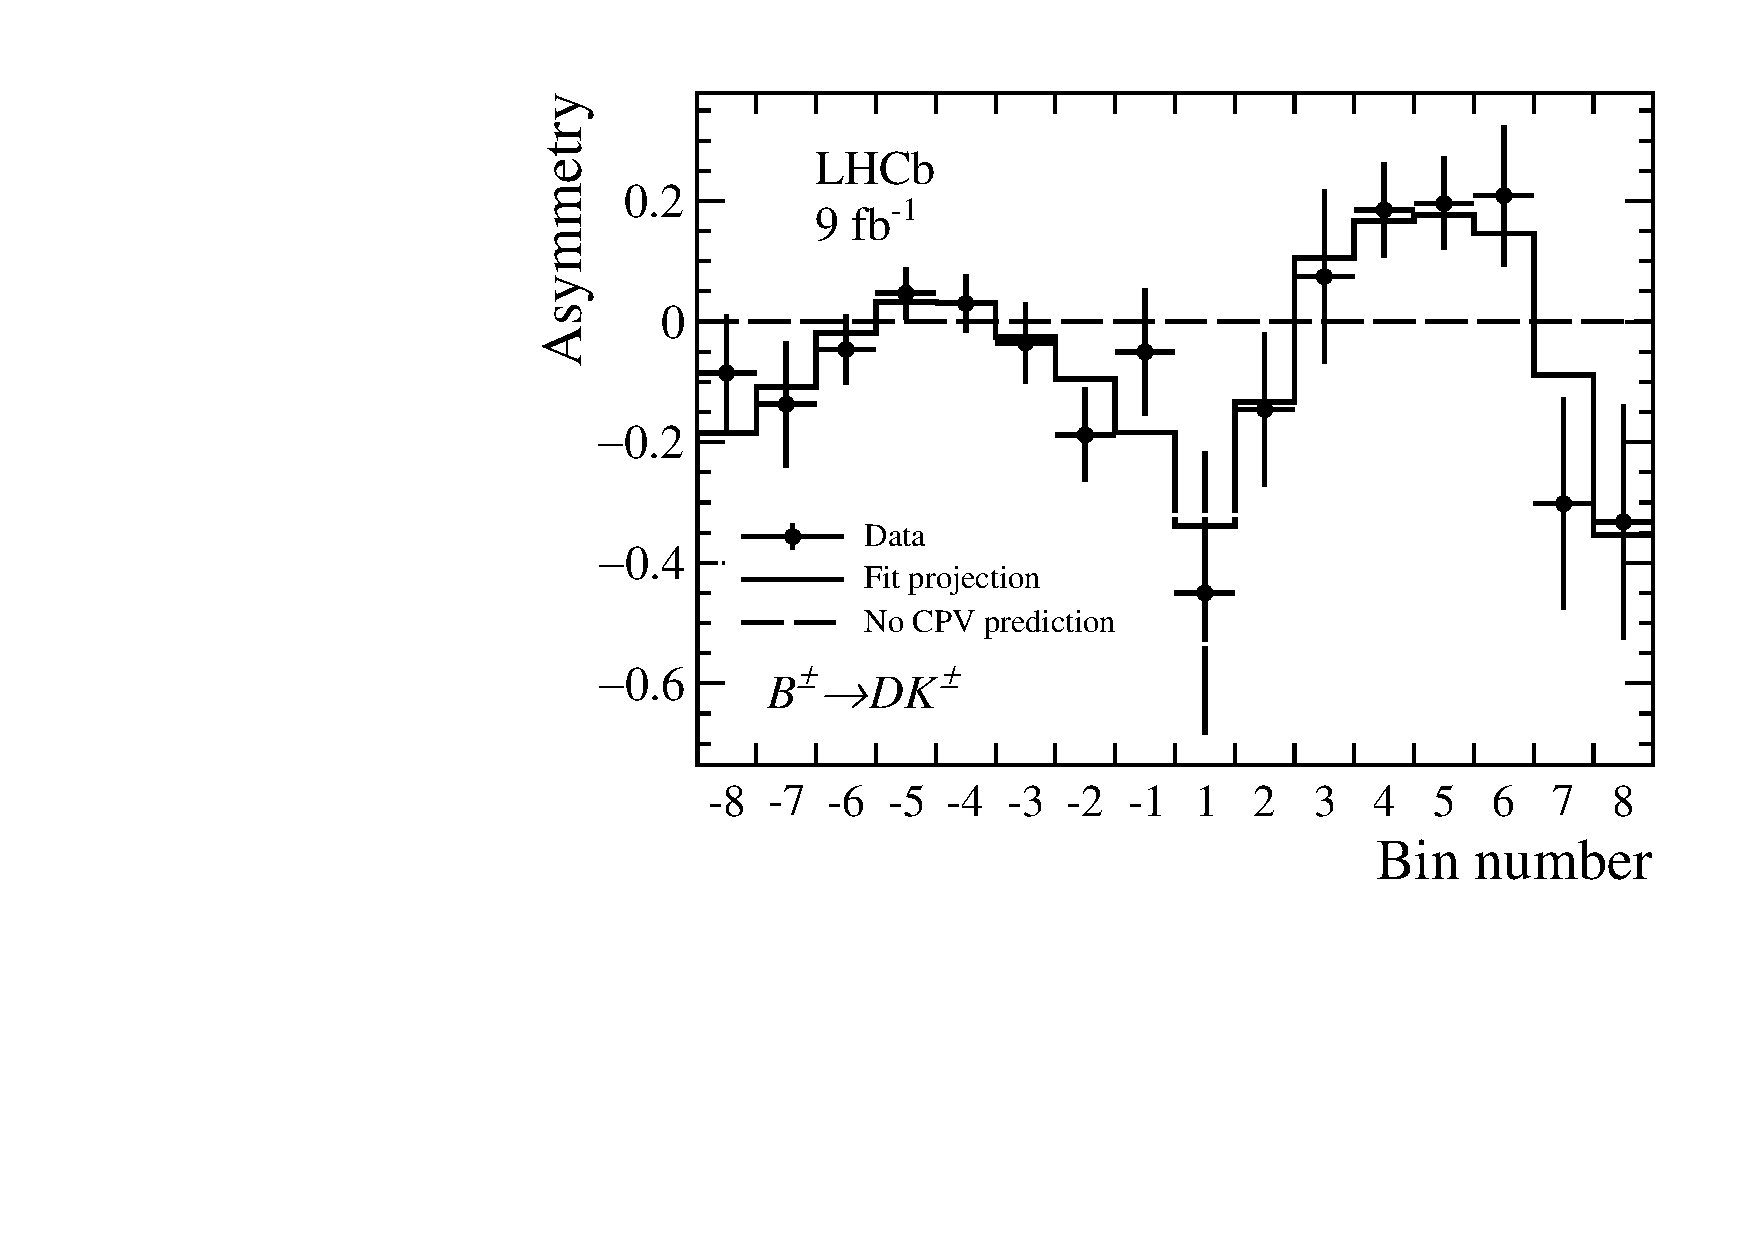
\includegraphics[width = 1.0\textwidth]{Plots/BinAsymmetries_dk.pdf}
      \caption{$B^\pm\to DK^\pm$}
    \end{subfigure}%
    \begin{subfigure}{0.5\textwidth}
      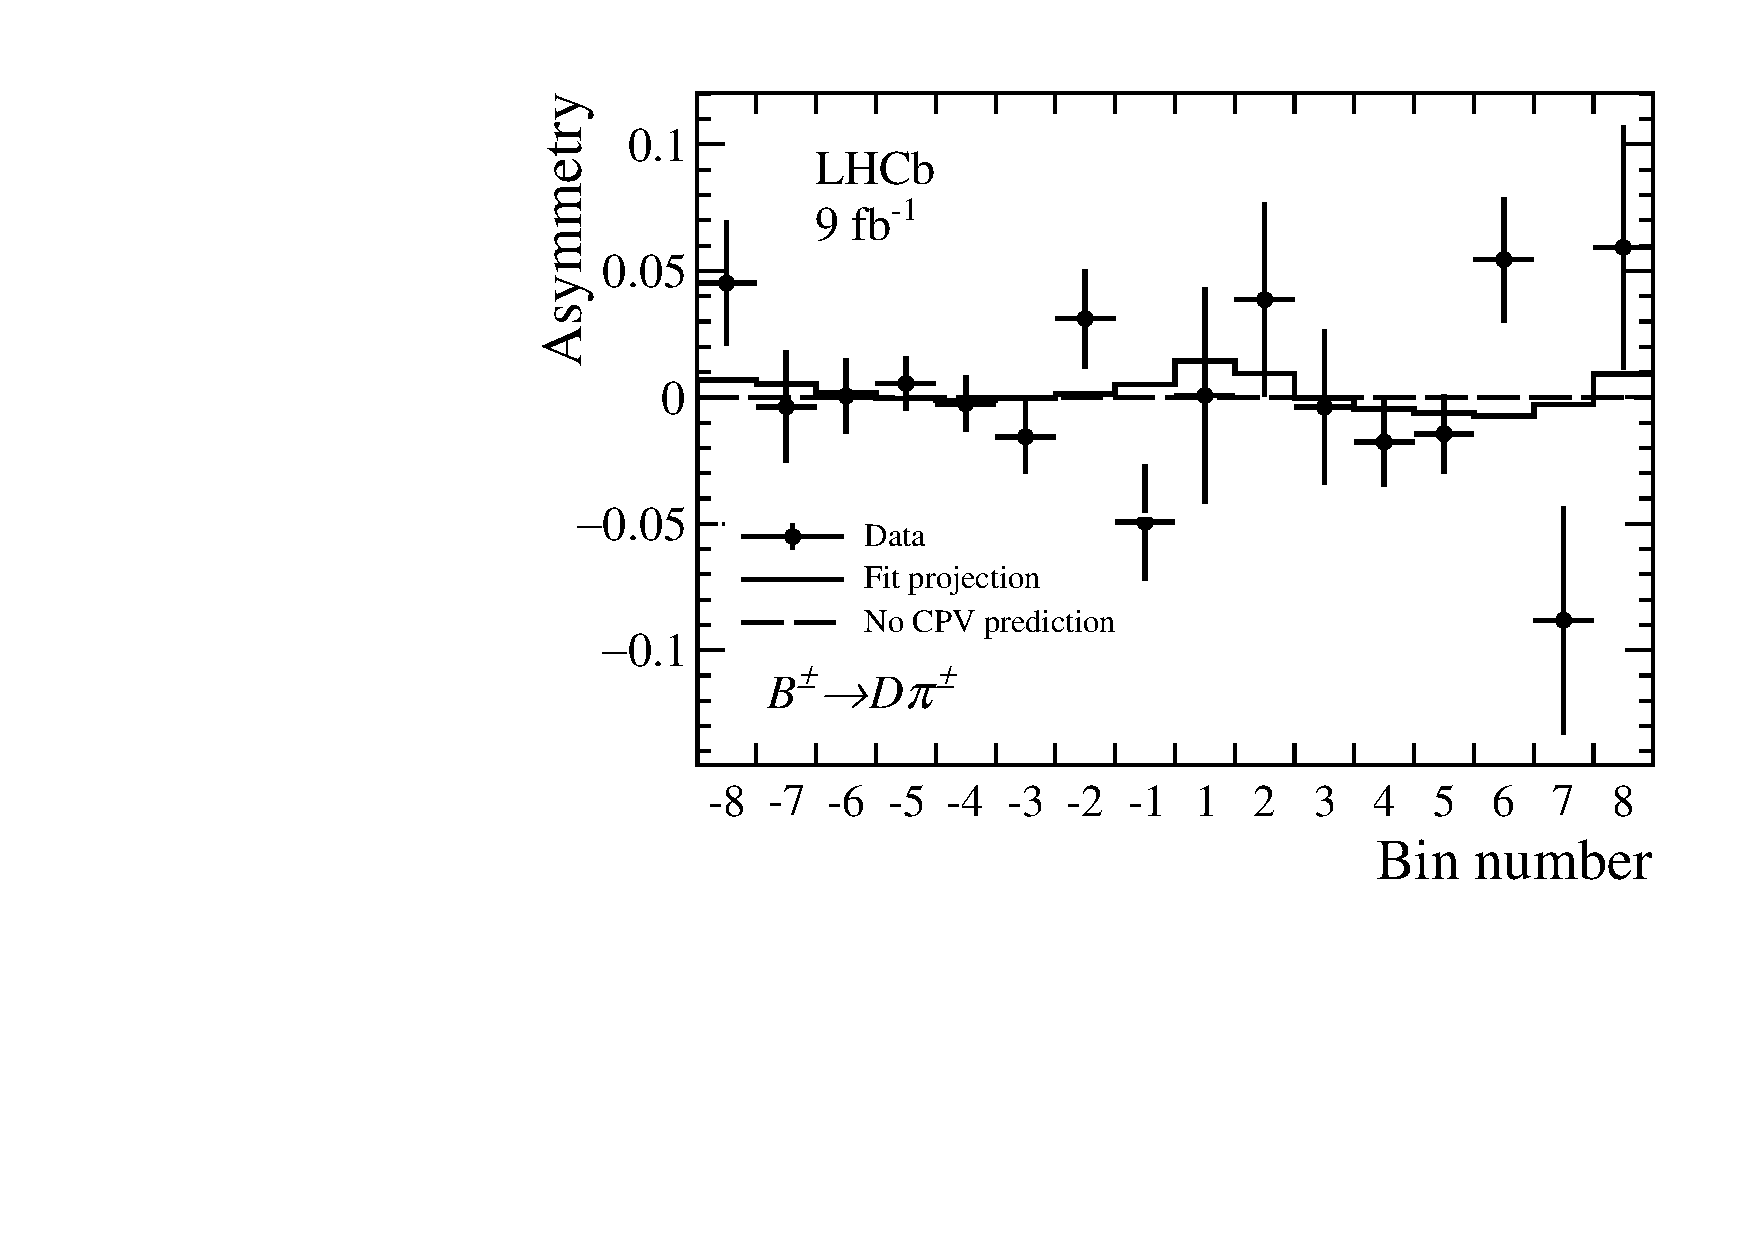
\includegraphics[width = 1.0\textwidth]{Plots/BinAsymmetries_dpi.pdf}
      \caption{$B^\pm\to D\pi^\pm$}
    \end{subfigure}
  \end{figure}
  \begin{itemize}
    \item{Useful cross check to compare measured bin asymmetries against bin asymmetries predicted by the fitted CP observables}
    \item{The $B^\pm\to DK^\pm$ mode show non-zero bin asymmetries, and the non-trivial distribution is driven by the change in strong phases across phase space}
  \end{itemize}
\end{frame}

\begin{frame}{CP fit results}
  \begin{figure}
    \centering
    \vspace{-0.2cm}
    \begin{subfigure}{0.5\textwidth}
      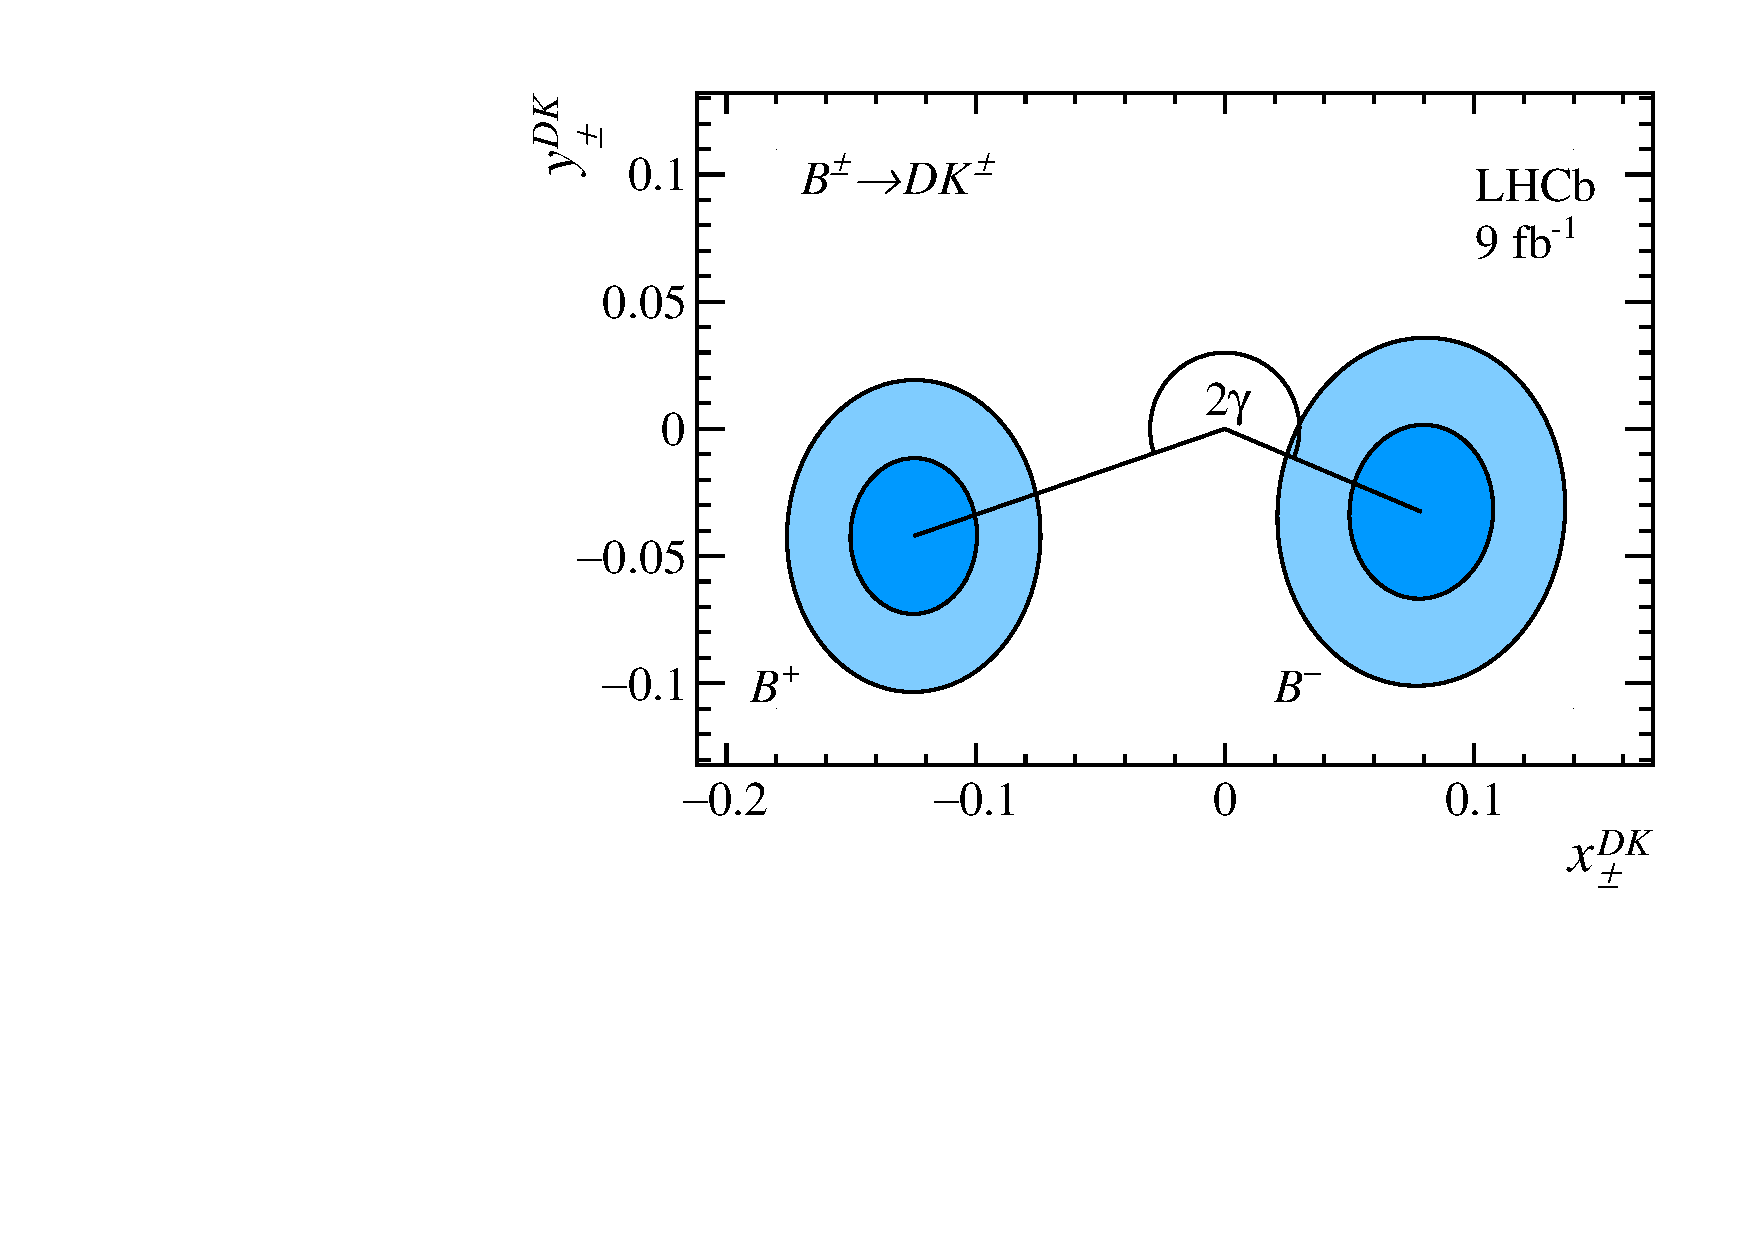
\includegraphics[width = 1.0\textwidth]{Plots/B2DK_CP_Observables_Contours.pdf}
      \caption{$x_\pm^{DK}$ vs $y_\pm^{DK}$}
    \end{subfigure}%
    \begin{subfigure}{0.5\textwidth}
      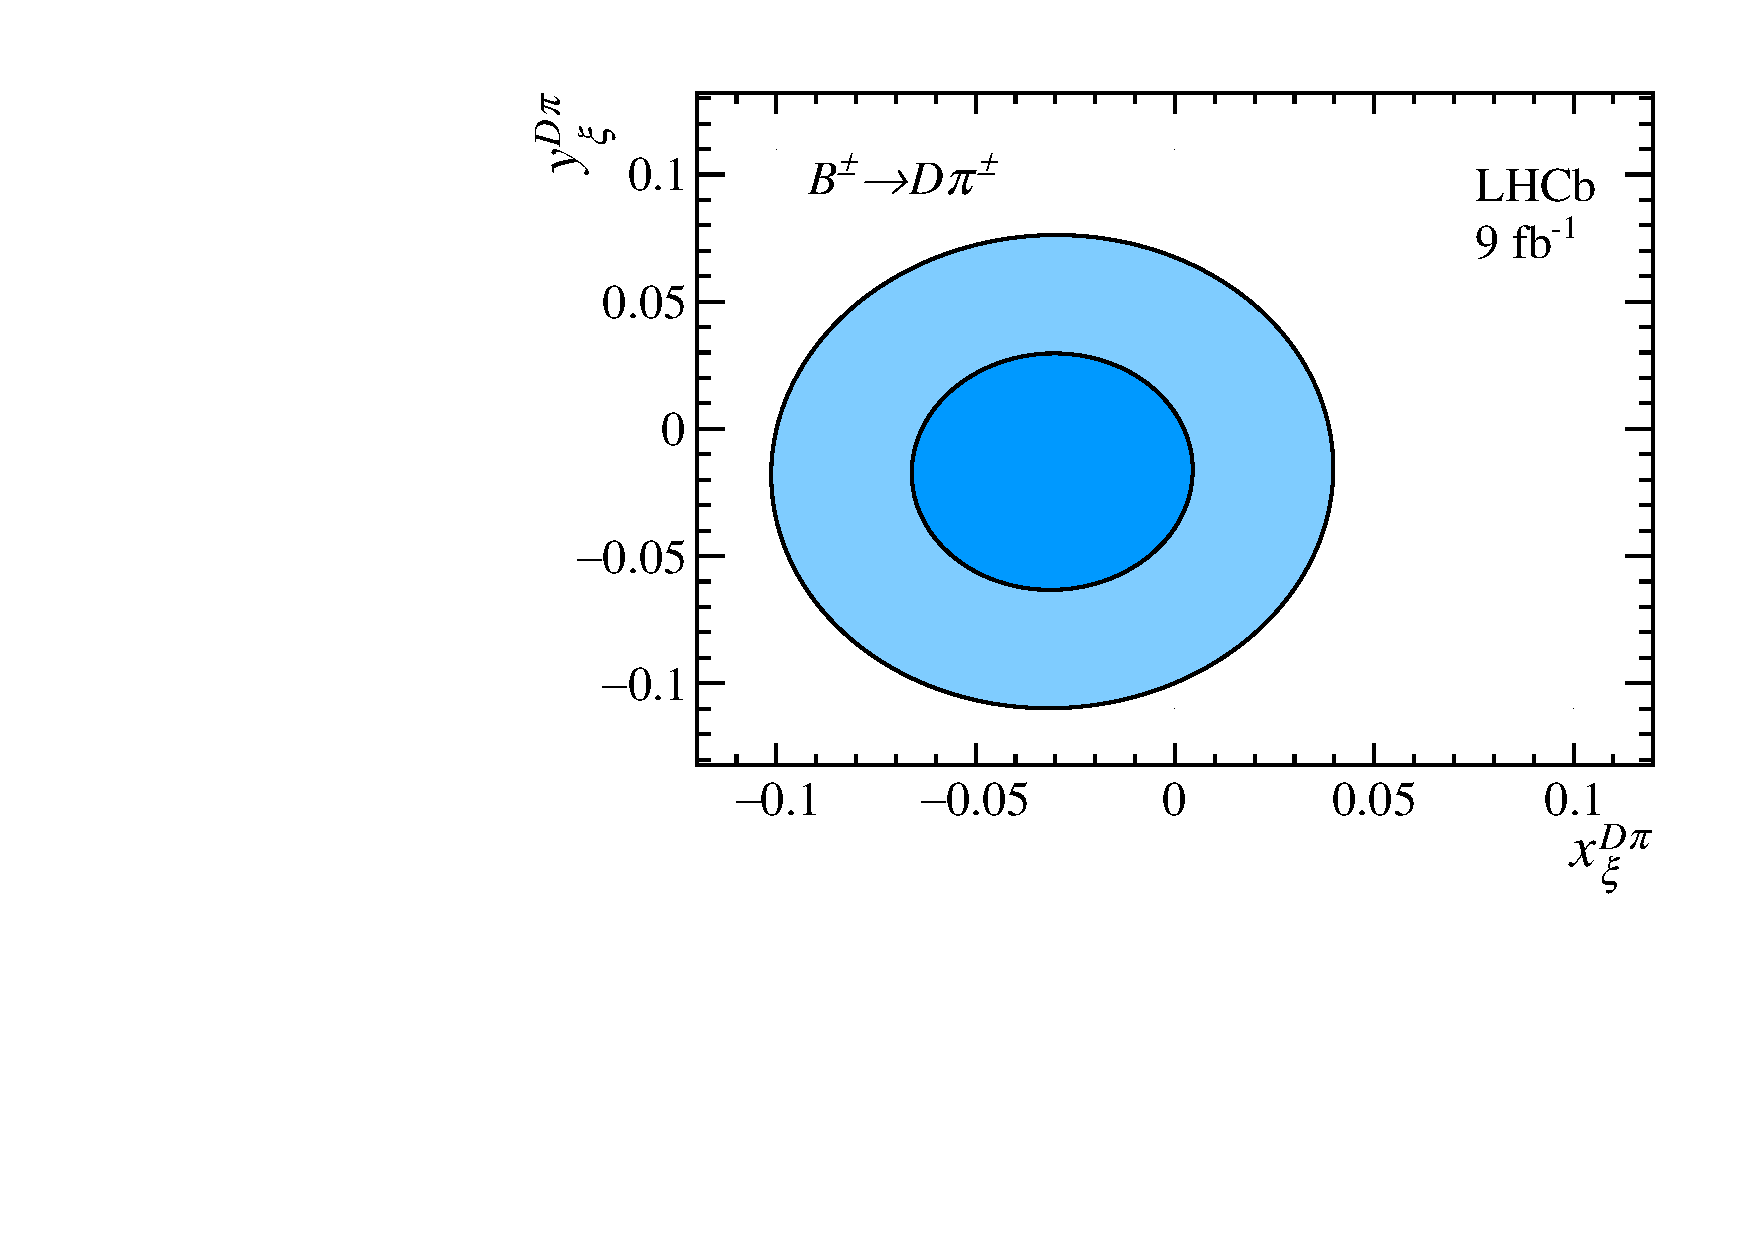
\includegraphics[width = 1.0\textwidth]{Plots/B2Dpi_CP_Observables_Contours.pdf}
      \caption{$x_\xi^{D\pi}$ vs $y_\xi^{D\pi}$}
    \end{subfigure}
  \end{figure}
  \vspace{-0.3cm}
  \begin{align*}
    x_\pm^{DK} = r_B\cos(\delta_B\pm\gamma) \\
    y_\pm^{DK} = r_B\sin(\delta_B\pm\gamma)
  \end{align*}
  \vspace{-0.5cm}
  \begin{itemize}
    \item{The $B^\pm\to DK^\pm$ contours are distinct, indicating $C\!P$ violation}
    \item{The $B^\pm\to D\pi^\pm$ mode has very low sensitivity to CP violation}
  \end{itemize}
\end{frame}

\begin{frame}{Interpretation of $\gamma$}
  \begin{center}
    \Large We can interpret our $C\!P$ observables in terms of the physics parameters $\gamma$, $r_B^{DK}$, $\delta_B^{DK}$, $r_B^{D\pi}$, $\delta_B^{D\pi}$
  \end{center}
  \begin{align*}
    \gamma &= (116^{+12}_{-14})^\circ, \\
    \delta_B^{DK} &= (81^{+14}_{-13})^\circ, \\
    r_B^{DK} &= 0.110^{+0.020}_{-0.020}, \\
    \delta_B^{D\pi} &= (298^{+62}_{-118})^\circ, \\
    r_B^{D\pi} &= 0.0041^{+0.0054}_{-0.0041},
  \end{align*}
  \begin{center}
    \large However, the latest $\gamma$ and charm combination result is:
  \end{center}
  \begin{equation*}
    \gamma = (63.8^{+3.5}_{-3.7})^\circ
  \end{equation*}
  \begin{center}
    \large What went wrong?!
  \end{center}  
\end{frame}

\begin{frame}{Interpretation of $\gamma$}
  \begin{figure}
    \centering
    \begin{overpic}[percent,scale=0.23]{Plots/SpongebobMemeTemplate.png}
      \put(7.5,75){\tiny$\gamma = (116^{+12}_{-14})^\circ$}
    \end{overpic}
  \end{figure}
  \begin{center}
    Do we trust the model predicted $c_i$ and $s_i$, or their uncertainties? No!
    \Large Let's go and measure $c_i$ and $s_i$ at BESIII!
  \end{center}
\end{frame}

\section{Strong phase analysis of \texorpdfstring{$D^0\to K^+K^-\pi^+\pi^-$}{D2KKpipi} at BESIII}
\begin{frame}{Strong phase analysis of $D^0\to K^+K^-\pi^+\pi^-$ at BESIII}
  \begin{center}
    {\huge Strong phase analysis of $D^0\to K^+K^-\pi^+\pi^-$ at BESIII}
  \end{center}
\end{frame}

\begin{frame}{Strong phase analysis of $D^0\to K^+K^-\pi^+\pi^-$ at BESIII}
  \begin{itemize}
    \item{BESIII: Beijing Spectrometer III, a detector at the Beijing Electron-Positron Collider II, located at IHEP}
    \item{$e^+e^-$ collider at the $\psi(3770)\to D^0\bar{D^0}$ threshold}
    \begin{itemize}
      \item{2010-2011: $\SI{3}{\per\femto\barn}$}
      \item{2022: $\SI{5}{\per\femto\barn}$}
      \item{Expect $\SI{20}{\per\femto\barn}$ in total by end of 2024}
    \end{itemize}
  \end{itemize}
  \begin{figure}
    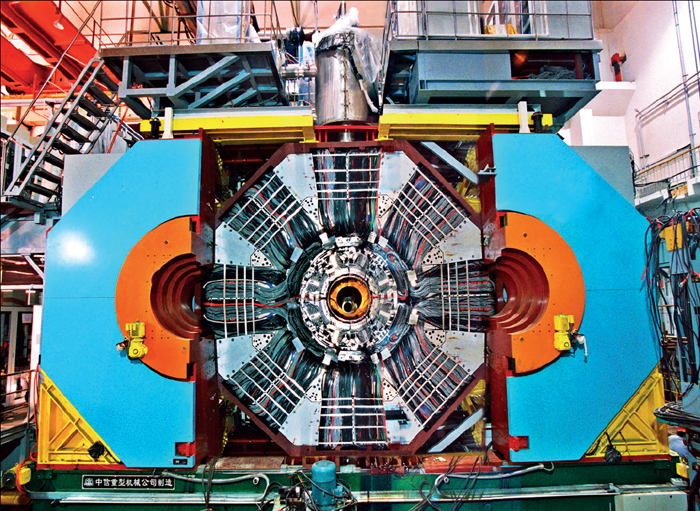
\includegraphics[width = 0.50\textwidth]{Plots/BESIIIDetector.jpg}
  \end{figure}
\end{frame}

\begin{frame}{Strong phase analysis of $D^0\to K^+K^-\pi^+\pi^-$ at BESIII}
  \begin{itemize}
    \item{Double-tag analysis: Reconstruct signal ($KK\pi\pi$) and tag mode}
    \item{$D^0\bar{D^0}$ pair is quantum correlated}
  \end{itemize}
  \begin{figure}[H]
    \centering
    \vspace{-1.5cm}
    \begin{fmffile}{fgraph/fgraph_ee1}
      \setlength{\unitlength}{1cm}
      \begin{fmfgraph*}(8,5)
        \fmfleft{i}
        \fmfright{o}
        \fmflabel{$D^0$}{i}
        \fmflabel{$\bar{D^0}$}{o}
        \fmf{fermion}{w,i}
        \fmf{fermion}{w,o}
        \fmfblob{1cm}{w}
        \fmfv{label=$\psi(3770)$,label.dist=15,label.angle=90}{w}
      \end{fmfgraph*}
    \end{fmffile}
    \vspace{-1.5cm}
  \end{figure}
  \begin{itemize}
    \item{Equivalently, we can consider $D_+D_-$}
    \begin{itemize}
      \item{$D_\pm = \frac{1}{\sqrt{2}}(D^0\pm\bar{D^0})$ are CP eigenstates}
    \end{itemize}
  \end{itemize}
  \begin{figure}[H]
    \centering
    \vspace{-1.5cm}
    \begin{fmffile}{fgraph/fgraph_ee2}
      \setlength{\unitlength}{1cm}
      \begin{fmfgraph*}(8,5)
        \fmfleft{i}
        \fmfright{o}
        \fmflabel{$D_+$}{i}
        \fmflabel{$D_-$}{o}
        \fmf{fermion}{w,i}
        \fmf{fermion}{w,o}
        \fmfblob{1cm}{w}
        \fmfv{label=$\psi(3770)$,label.dist=15,label.angle=90}{w}
      \end{fmfgraph*}
    \end{fmffile}
    \vspace{-1.5cm}
  \end{figure}
  \begin{center}
    The $DD$ pair is \underline{quantum correlated}, spooky action at a distance!
  \end{center}
\end{frame}

\begin{frame}{Strong-phase in quantum correlated $D^0\bar{D^0}$ decays}
  \begin{itemize}
    \item{Tag mode can be a \underline{flavour tag}}
    \begin{itemize}
      \item{$K^-\pi^+$, $K^-\pi^+\pi^0$, $K^-\pi^+\pi^-\pi^+$, $K^-e^+\nu_e$}
    \end{itemize}
  \end{itemize}
  \begin{figure}[H]
    \centering
    \vspace{0.3cm}
    \begin{fmffile}{fgraph/fgraph_flavour_tag}
      \setlength{\unitlength}{1cm}
      \begin{fmfgraph*}(8,4)
        \fmfstraight
        \fmfleft{i4,i3,i2,i1}
        \fmfright{g1,o1,o2,g2}
        \fmflabel{$\pi^+$}{o1}
        \fmflabel{$K^-$}{o2}
        \fmflabel{$K^+$}{i1}
        \fmflabel{$K^-$}{i2}
        \fmflabel{$\pi^+$}{i3}
        \fmflabel{$\pi^-$}{i4}
        \fmf{fermion}{w,i1}
        \fmf{fermion}{w,i2}
        \fmf{fermion}{w,i3}
        \fmf{fermion}{w,i4}
        \fmf{fermion}{w,o1}
        \fmf{fermion}{w,o2}
        \fmf{phantom}{w,g1}
        \fmf{phantom}{w,g2}
        \fmfblob{1cm}{w}
      \end{fmfgraph*}
    \end{fmffile}
    \vspace{0.3cm}
  \end{figure}
  \begin{center}
    Flavour tags do not exhibit \underline{quantum correlation} effects
  \end{center}
\end{frame}

\begin{frame}{Strong-phases in quantum correlated $D^0\bar{D^0}$ decays}
  \begin{itemize}
    \item{Tag mode can be a \underline{CP even tag}}
    \begin{itemize}
      \item{$KK$, $\pi\pi$, $\pi\pi\pi^0$, $K_S\pi^0\pi^0$, $K_L\pi^0$, $K_L\omega$}
    \end{itemize}
  \end{itemize}
  \begin{figure}[H]
    \centering
    \vspace{0.3cm}
    \begin{fmffile}{fgraph/fgraph_CPeven_tag}
      \setlength{\unitlength}{1cm}
      \begin{fmfgraph*}(8,4)
        \fmfstraight
        \fmfleft{i4,i3,i2,i1}
        \fmfright{g1,o1,o2,g2}
        \fmflabel{$K^+$}{o1}
        \fmflabel{$K^-$}{o2}
        \fmflabel{$K^+$}{i1}
        \fmflabel{$K^-$}{i2}
        \fmflabel{$\pi^+$}{i3}
        \fmflabel{$\pi^-$}{i4}
        \fmf{fermion}{w,i1}
        \fmf{fermion}{w,i2}
        \fmf{fermion}{w,i3}
        \fmf{fermion}{w,i4}
        \fmf{fermion}{w,o1}
        \fmf{fermion}{w,o2}
        \fmf{phantom}{w,g1}
        \fmf{phantom}{w,g2}
        \fmfblob{1cm}{w}
      \end{fmfgraph*}
    \end{fmffile}
    \vspace{0.3cm}
  \end{figure}
  \begin{center}
    $D\to K^+K^-$, which is $C\!P$ even, forces $D\to K^+K^-\pi^+\pi^-$ to be $C\!P$ odd
  \end{center}
\end{frame}

\begin{frame}{Strong-phase in quantum correlated $D^0\bar{D^0}$ decays}
  \begin{itemize}
    \item{Tag mode can be a \underline{CP odd tag}}
    \begin{itemize}
      \item{$K_S\pi^0$, $K_S\omega$, $K_S\eta$, $K_S\eta'$, $K_L\pi^0\pi^0$}
    \end{itemize}
  \end{itemize}
  \begin{figure}[H]
    \centering
    \vspace{0.3cm}
    \begin{fmffile}{fgraph/fgraph_CPodd_tag}
      \setlength{\unitlength}{1cm}
      \begin{fmfgraph*}(8,4)
        \fmfstraight
        \fmfleft{i4,i3,i2,i1}
        \fmfright{g1,o1,o2,g2}
        \fmflabel{$\pi^0$}{o1}
        \fmflabel{$K_S$}{o2}
        \fmflabel{$K^+$}{i1}
        \fmflabel{$K^-$}{i2}
        \fmflabel{$\pi^+$}{i3}
        \fmflabel{$\pi^-$}{i4}
        \fmf{fermion}{w,i1}
        \fmf{fermion}{w,i2}
        \fmf{fermion}{w,i3}
        \fmf{fermion}{w,i4}
        \fmf{fermion}{w,o1}
        \fmf{fermion}{w,o2}
        \fmf{phantom}{w,g1}
        \fmf{phantom}{w,g2}
        \fmfblob{1cm}{w}
      \end{fmfgraph*}
    \end{fmffile}
    \vspace{0.3cm}
  \end{figure}
  \begin{center}
    $D\to K_S^0\pi^0$, which is $C\!P$ odd, forces $D\to K^+K^-\pi^+\pi^-$ to be $C\!P$ even
  \end{center}
\end{frame}

\begin{frame}{Strong phase analysis of $D^0\to K^+K^-\pi^+\pi^-$ at BESIII}
  \begin{center}
    Quantum correlation can modify the effective branching fraction:
  \end{center}
  \begin{equation*}
    \frac{N^{\rm DT}}{N^{\rm ST}} = \mathcal{B}(D^0\to KK\pi\pi)\big(1\pm c_1\big)
  \end{equation*}
  \begin{figure}
    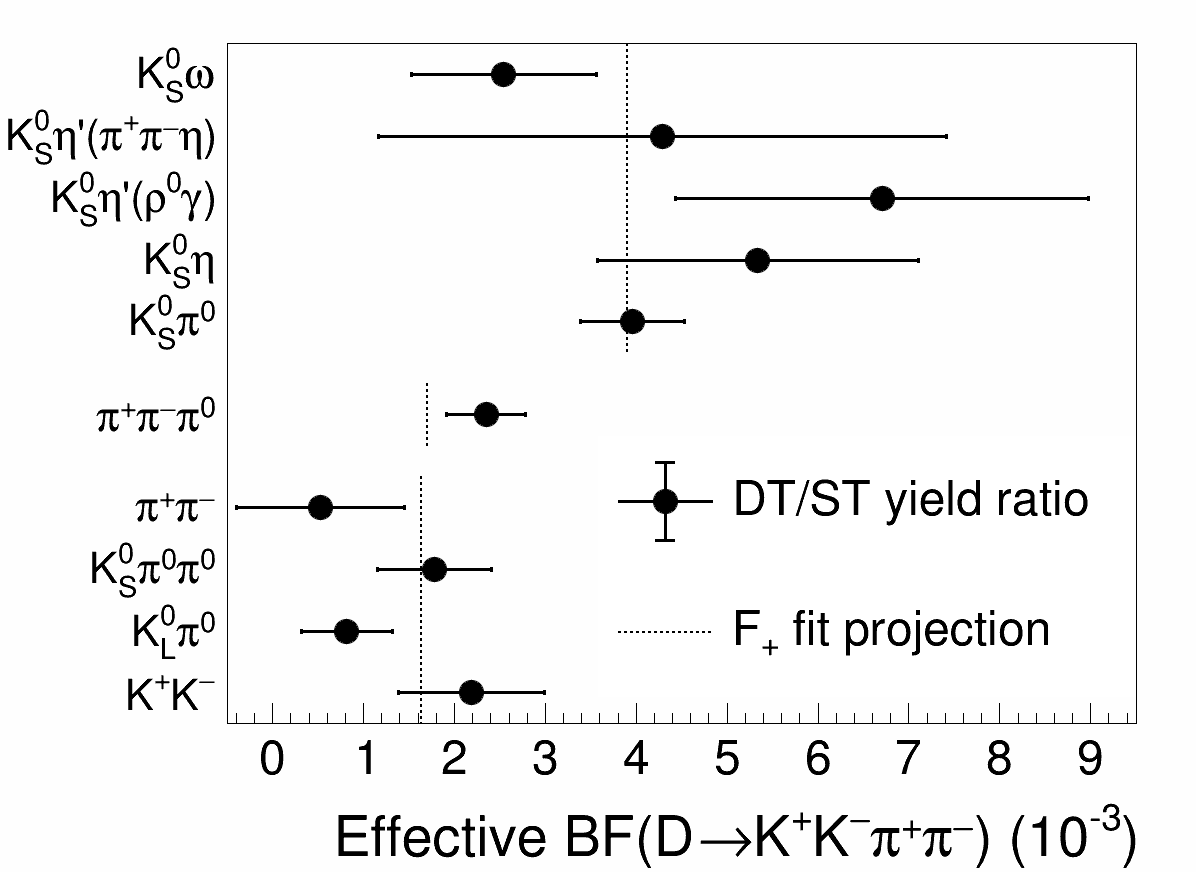
\includegraphics[width = 0.50\textwidth]{Plots/CPeven_fraction_combination_CPtags.png}
    \caption*{\tiny arXiv:2212.06489}
  \end{figure}
  \vspace{-0.3cm}
  \begin{center}
    $c_1$ is the cosine of the strong phase, averaged over the \underline{whole} phase space
  \end{center}
\end{frame}

\begin{frame}{Strong phase analysis of $D^0\to K^+K^-\pi^+\pi^-$ at BESIII}
  \begin{center}
    Our next task is to change the phase space inclusive analysis,
  \end{center}
  \vspace{-0.5cm}
  \begin{align*}
    \frac{N^{\rm DT}}{N^{\rm ST}} =& \mathcal{B}(D^0\to KK\pi\pi)\quad\textnormal{(flavour tag)} \\
    \frac{N^{\rm DT}}{N^{\rm ST}} =& \mathcal{B}(D^0\to KK\pi\pi)\big(1\pm c_1\big)\quad\textnormal{(CP tag)}
  \end{align*}
  \vspace{-1.0cm}
  \begin{center}
    into a binned phase space analysis:
  \end{center}
  \vspace{-0.6cm}
  \begin{align*}
    \frac{N^{\rm DT}_i}{N^{\rm ST}} =& \mathcal{B}(D^0\to KK\pi\pi)F_i\quad\textnormal{(flavour tag)} \\
    \frac{N^{\rm DT}_i}{N^{\rm ST}} =& \mathcal{B}(D^0\to KK\pi\pi)\big(F_i + \bar{F_i} \pm 2\sqrt{F_i\bar{F_i}}c_i\big)\quad\textnormal{(CP tag)}
  \end{align*}
  \vspace{-0.6cm}
  \begin{enumerate}
    \item{$F_i$: Measure using flavour tags}
    \item{$c_i$: Determine from asymmetry of $C\!P$ even and odd tags}
    \item[]{\phantom{$s_i$: Analogous to $c_i$, but requires binning of tag mode}}
  \end{enumerate}
  \vspace{-7.0cm}
  \begin{center}
    \phantom{\rotatebox{45}{\Huge\colorbox{white}{\framebox{Work in progress!}}}}
  \end{center}
\end{frame}

\begin{frame}{Strong phase analysis of $D^0\to K^+K^-\pi^+\pi^-$ at BESIII}
  \begin{center}
    Our next task is to change the phase space inclusive analysis,
  \end{center}
  \vspace{-0.5cm}
  \begin{align*}
    \frac{N^{\rm DT}}{N^{\rm ST}} =& \mathcal{B}(D^0\to KK\pi\pi)\quad\textnormal{(flavour tag)} \\
    \frac{N^{\rm DT}}{N^{\rm ST}} =& \mathcal{B}(D^0\to KK\pi\pi)\big(1\pm c_1\big)\quad\textnormal{(CP tag)}
  \end{align*}
  \vspace{-1.0cm}
  \begin{center}
    into a binned phase space analysis:
  \end{center}
  \vspace{-0.6cm}
  \begin{align*}
    \frac{N^{\rm DT}_i}{N^{\rm ST}} =& \mathcal{B}(D^0\to KK\pi\pi)F_i\quad\textnormal{(flavour tag)} \\
    \frac{N^{\rm DT}_i}{N^{\rm ST}} =& \mathcal{B}(D^0\to KK\pi\pi)\big(F_i + \bar{F_i} \pm 2\sqrt{F_i\bar{F_i}}c_i\big)\quad\textnormal{(CP tag)}
  \end{align*}
  \vspace{-0.6cm}
  \begin{enumerate}
    \item{$F_i$: Measure using flavour tags}
    \item{$c_i$: Determine from asymmetry of $C\!P$ even and odd tags}
    \item{$s_i$: Analogous to $c_i$, but requires binning of tag mode}
  \end{enumerate}
  \vspace{-7.0cm}
  \begin{center}
    \phantom{\rotatebox{45}{\Huge\colorbox{white}{\framebox{Work in progress!}}}}
  \end{center}
\end{frame}

\begin{frame}{Strong phase analysis of $D^0\to K^+K^-\pi^+\pi^-$ at BESIII}
  \begin{center}
    Our next task is to change the phase space inclusive analysis,
  \end{center}
  \vspace{-0.5cm}
  \begin{align*}
    \frac{N^{\rm DT}}{N^{\rm ST}} =& \mathcal{B}(D^0\to KK\pi\pi)\quad\textnormal{(flavour tag)} \\
    \frac{N^{\rm DT}}{N^{\rm ST}} =& \mathcal{B}(D^0\to KK\pi\pi)\big(1\pm c_1\big)\quad\textnormal{(CP tag)}
  \end{align*}
  \vspace{-1.0cm}
  \begin{center}
    into a binned phase space analysis:
  \end{center}
  \vspace{-0.6cm}
  \begin{align*}
    \frac{N^{\rm DT}_i}{N^{\rm ST}} =& \mathcal{B}(D^0\to KK\pi\pi)F_i\quad\textnormal{(flavour tag)} \\
    \frac{N^{\rm DT}_i}{N^{\rm ST}} =& \mathcal{B}(D^0\to KK\pi\pi)\big(F_i + \bar{F_i} \pm 2\sqrt{F_i\bar{F_i}}c_i\big)\quad\textnormal{(CP tag)}
  \end{align*}
  \vspace{-0.6cm}
  \begin{enumerate}
    \item{$F_i$: Measure using flavour tags}
    \item{$c_i$: Determine from asymmetry of $C\!P$ even and odd tags}
    \item{$s_i$: Analogous to $c_i$, but requires binning of tag mode}
  \end{enumerate}
  \vspace{-7.0cm}
  \begin{center}
    \rotatebox{45}{\Huge\colorbox{white}{\framebox{Work in progress!}}}
  \end{center}
\end{frame}

\section{Summary and conclusion}
\begin{frame}{Summary and conclusion}
  \begin{enumerate}
    \setlength\itemsep{1.5em}
    \item{I have presented a CPV study of $B^\pm\to[K^+K^-\pi^+\pi^-]_Dh^\pm$}
    \item{Multi-body decays, such as $D^0\to K^+K^-\pi^+\pi^-$, have a great potential for measuring $\gamma$}
    \item{The optimised binning scheme, developed with an amplitude model, successfully identified regions with large, local $C\!P$ asymmetries}
  \end{enumerate}
  \begin{columns}[onlytextwidth]
    \begin{column}{0.5\textwidth}
      \centering
      \begin{enumerate}
        \setcounter{enumi}{3}
        \item{However, amplitude model predictions of $\delta_D$ \underline{should not be trusted}}
      \end{enumerate}
    \end{column}
    \begin{column}{0.5\textwidth}
      \begin{figure}
        \begin{overpic}[percent,scale=0.2]{Plots/SpongebobAmplitudeModel.png}
          \put(58,64){\small Making binning}
          \put(58,56){\small scheme with}
          \put(58,48){\small amplitude model}
          \put(58,30){\small Predicting strong}
          \put(58,22){\small phases with}
          \put(58,14){\small amplitude model}
        \end{overpic}
      \end{figure}
    \end{column}
  \end{columns}
\end{frame}

\begin{frame}{Summary and conclusion}
  \begin{enumerate}
    \setlength\itemsep{1.0em}
    \setcounter{enumi}{4}
    \item{The fit results, using model predicted strong phases, were found to have a $3\sigma$ tension with the current LHCb combination}
    \item{External inputs from charm factories, such as BESIII, are crucial to constrain charm strong phases}
    \item{Combined, the LHCb and BESIII analyses will lead to the first model independent measurement of $\gamma$ in this channel}
    \item{Work is ongoing in similar four-body modes:}
    \begin{itemize}
      \item{$D^0\to\pi^+\pi^-\pi^+\pi^-$}
      \item{$D^0\to K_S^0\pi^+\pi^-\pi^0$}
    \end{itemize}
  \end{enumerate}
  \vspace{0.2cm}
  \begin{center}
    {\huge Thanks for your attention!}
  \end{center}
\end{frame}

\section{Backup slides}
\begin{frame}{Backup slides}
  \begin{center}
    {\huge Backup slides}
  \end{center}
\end{frame}

\begin{frame}{The LHCb detector}
  \begin{center}
    {\huge The LHCb detector}
  \end{center}
\end{frame}

\begin{frame}{The LHCb detector}
  \begin{figure}
    \centering
    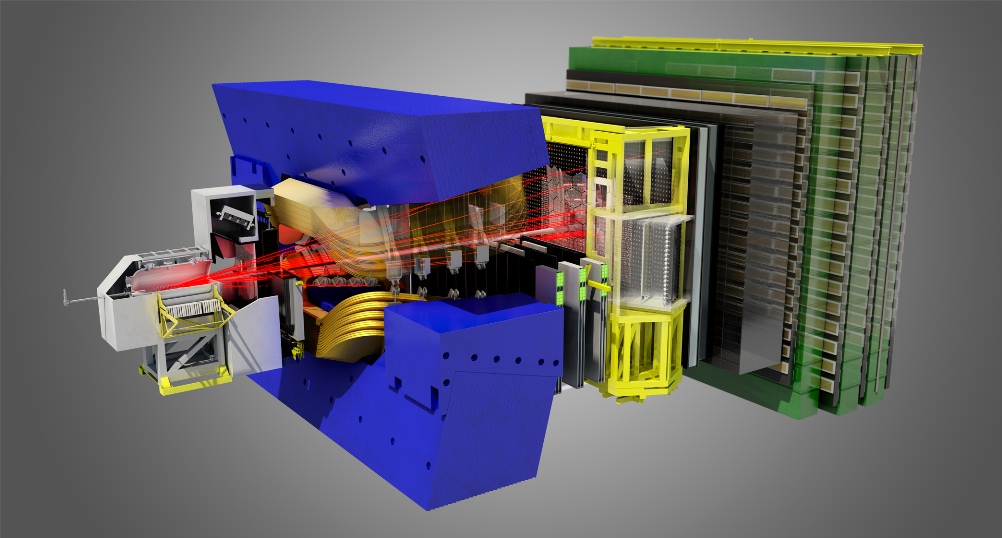
\includegraphics[width = 0.7\textwidth]{Plots/LHCbDetector.png}
  \end{figure}
  \begin{center}
    \Large LHCb: A beauty experiment with a lot of charm
  \end{center}
\end{frame}

\begin{frame}{The LHCb detector}
  \begin{figure}
    \centering
    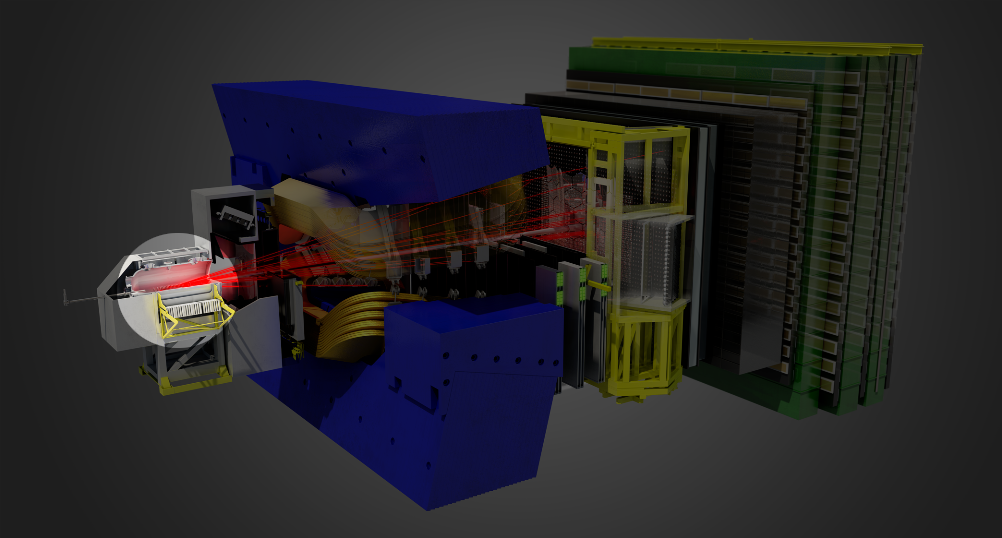
\includegraphics[width = 0.7\textwidth]{Plots/LHCbDetector_VELO.png}
  \end{figure}
  \begin{center}
    \Large VELO: Vertex locator to reconstruct $B$ and $D$ vertices
  \end{center}
\end{frame}

\begin{frame}{The LHCb detector}
  \begin{figure}
    \centering
    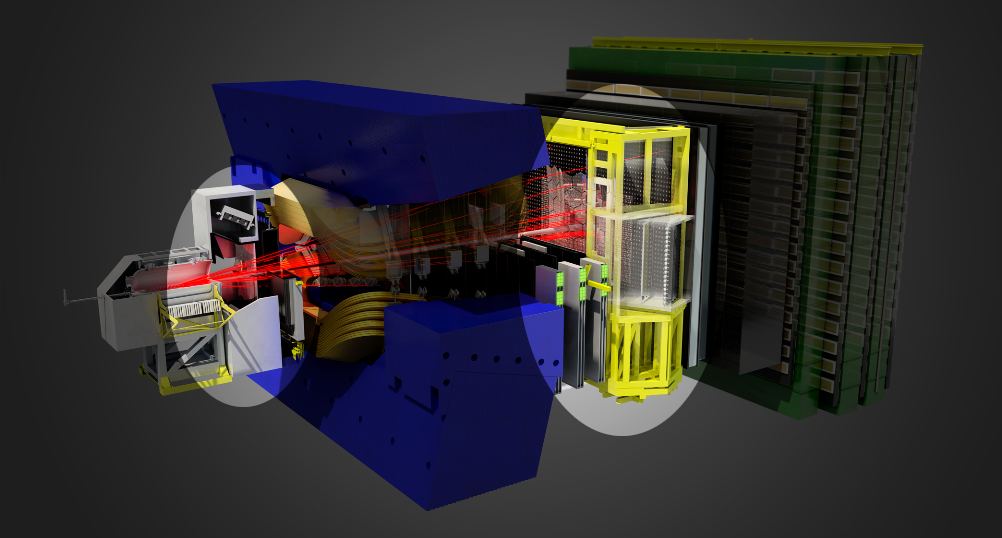
\includegraphics[width = 0.7\textwidth]{Plots/LHCbDetector_RICH.png}
  \end{figure}
  \begin{center}
    \Large RICH: Identify $B$ and $D$ daughter particles
  \end{center}
\end{frame}

\begin{frame}{Event selection}
  \begin{center}
    {\huge Event selection}
  \end{center}
\end{frame}

\begin{frame}{Event selection}
  \begin{center}
    \Large Decay topology
  \end{center}
  \vspace{0.5cm}
  \begin{columns}
    \begin{column}{0.4\textwidth}
      Look for:
      \begin{enumerate}
        \item{5 charged tracks}
        \item{Displaced $B$ vertex}
        \item{1 bachelor track with good PID information}
        \item{Displaced $D$ vertex with invariant mass within $\SI{25}{\mega\eV}$ of the $D^0$ mass}
      \end{enumerate}
    \end{column}
    \begin{column}{0.6\textwidth}
      \begin{figure}[H]
        \centering
        \begin{fmffile}{fgraph/fgraph_DecayTopology}
          \setlength{\unitlength}{0.4cm}
          \begin{fmfgraph*}(9,9)
            \fmfleft{i1,i2,i3}
            \fmfv{decor.shape=circle,decor.filled=shaded,decor.size=0.2w,label=IP,label.angle=180,label.dist=0.5cm}{i1}
            \fmfright{o1,o2,o3,o4,o5}
            \fmflabel{$\pi^+$}{o1}
            \fmflabel{$\pi^-$}{o2}
            \fmflabel{$K^+$}{o3}
            \fmflabel{$K^-$}{o4}
            \fmflabel{$K^-$}{o5}
            \fmf{phantom,tension=1.5}{i3,v1}
            \fmf{dashes,tension=2.5}{i1,v1}
            \fmfv{decor.shape=circle,decor.filled=shaded,decor.size=0.15w,label=$B^-$,label.angle=110,label.dist=0.5cm}{v1}
            \fmf{plain}{v1,o5}
            \fmf{dashes,tension=1.5}{v1,v2}
            \fmfv{decor.shape=circle,decor.filled=shaded,decor.size=0.15w,label=$D$,label.angle=-110,label.dist=0.5cm}{v2}
            \fmf{plain}{v2,o1}
            \fmf{plain}{v2,o2}
            \fmf{plain}{v2,o3}
            \fmf{plain}{v2,o4}
          \end{fmfgraph*}
        \end{fmffile}
        \vspace{0.5cm}
      \end{figure}
    \end{column}
  \end{columns}
\end{frame}

\begin{frame}{Event selection}
  \begin{center}
    \large Offline selection has 3 stages
  \end{center}
  Initial cuts:
  \begin{enumerate}
    \item{Invariant $D$ and $B$ mass cuts}
    \item{Momentum and RICH requirements}
  \end{enumerate}
  Boosted Decision Tree (BDT)
  \begin{itemize}
    \item{Signal sample: Simulation samples}
    \item{Background sample: Upper $B$ mass sideband}
    \item{28 variables describing kinematics, impact parameters, vertex quality}
  \end{itemize}
  Final selection
  \begin{enumerate}
    \item{$D$ Flight distance}
    \item{Particle Identification of bachelor}
    \item{$K_S^0$ veto}
  \end{enumerate}
\end{frame}

\begin{frame}{Event selection}
  \begin{figure}
    \centering
    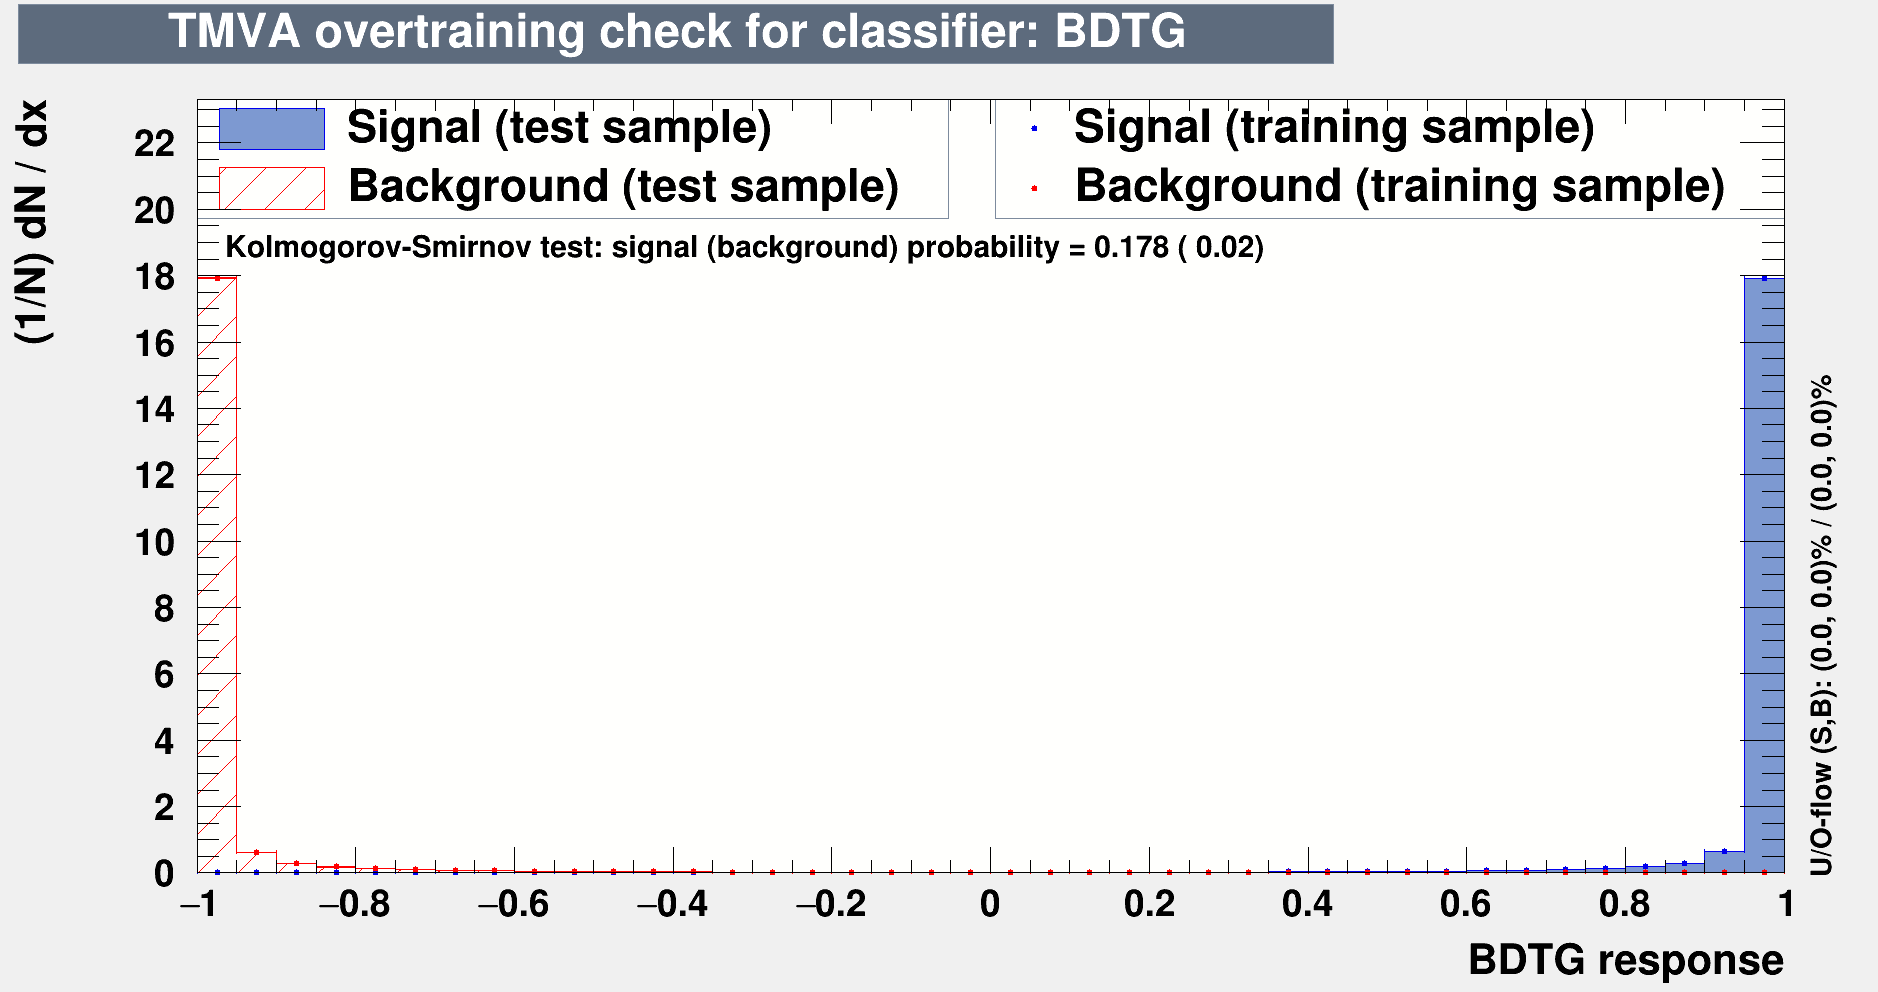
\includegraphics[width = 1.0\textwidth]{Plots/overtrain_BDTG.png}
  \end{figure}
  \begin{center}
    BDT is highly efficient at rejecting combinatorial background
  \end{center}
\end{frame}

\begin{frame}{Event selection}
  \begin{figure}
    \centering
    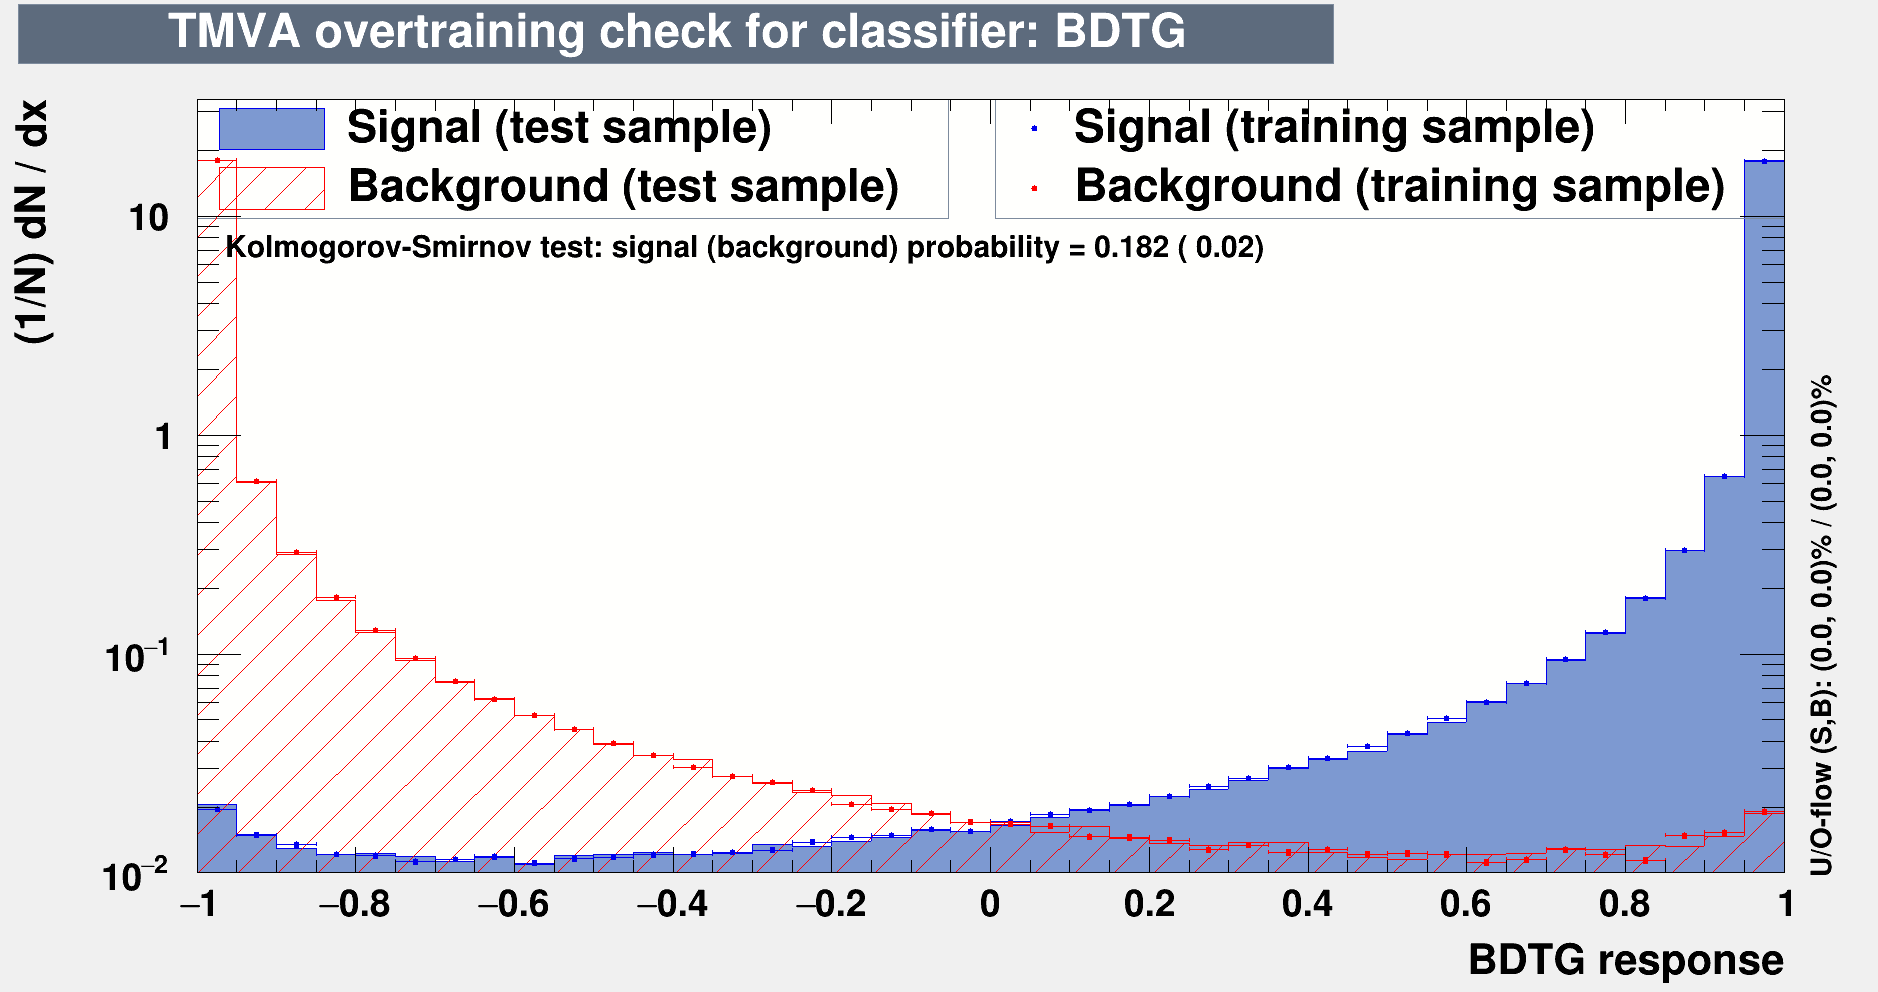
\includegraphics[width = 1.0\textwidth]{Plots/overtrain_BDTG_log.png}
  \end{figure}
  \begin{center}
    Very important, combinatorial background is large in multi-body decays
  \end{center}
\end{frame}

\begin{frame}{Event selection}
  \begin{figure}
    \centering
    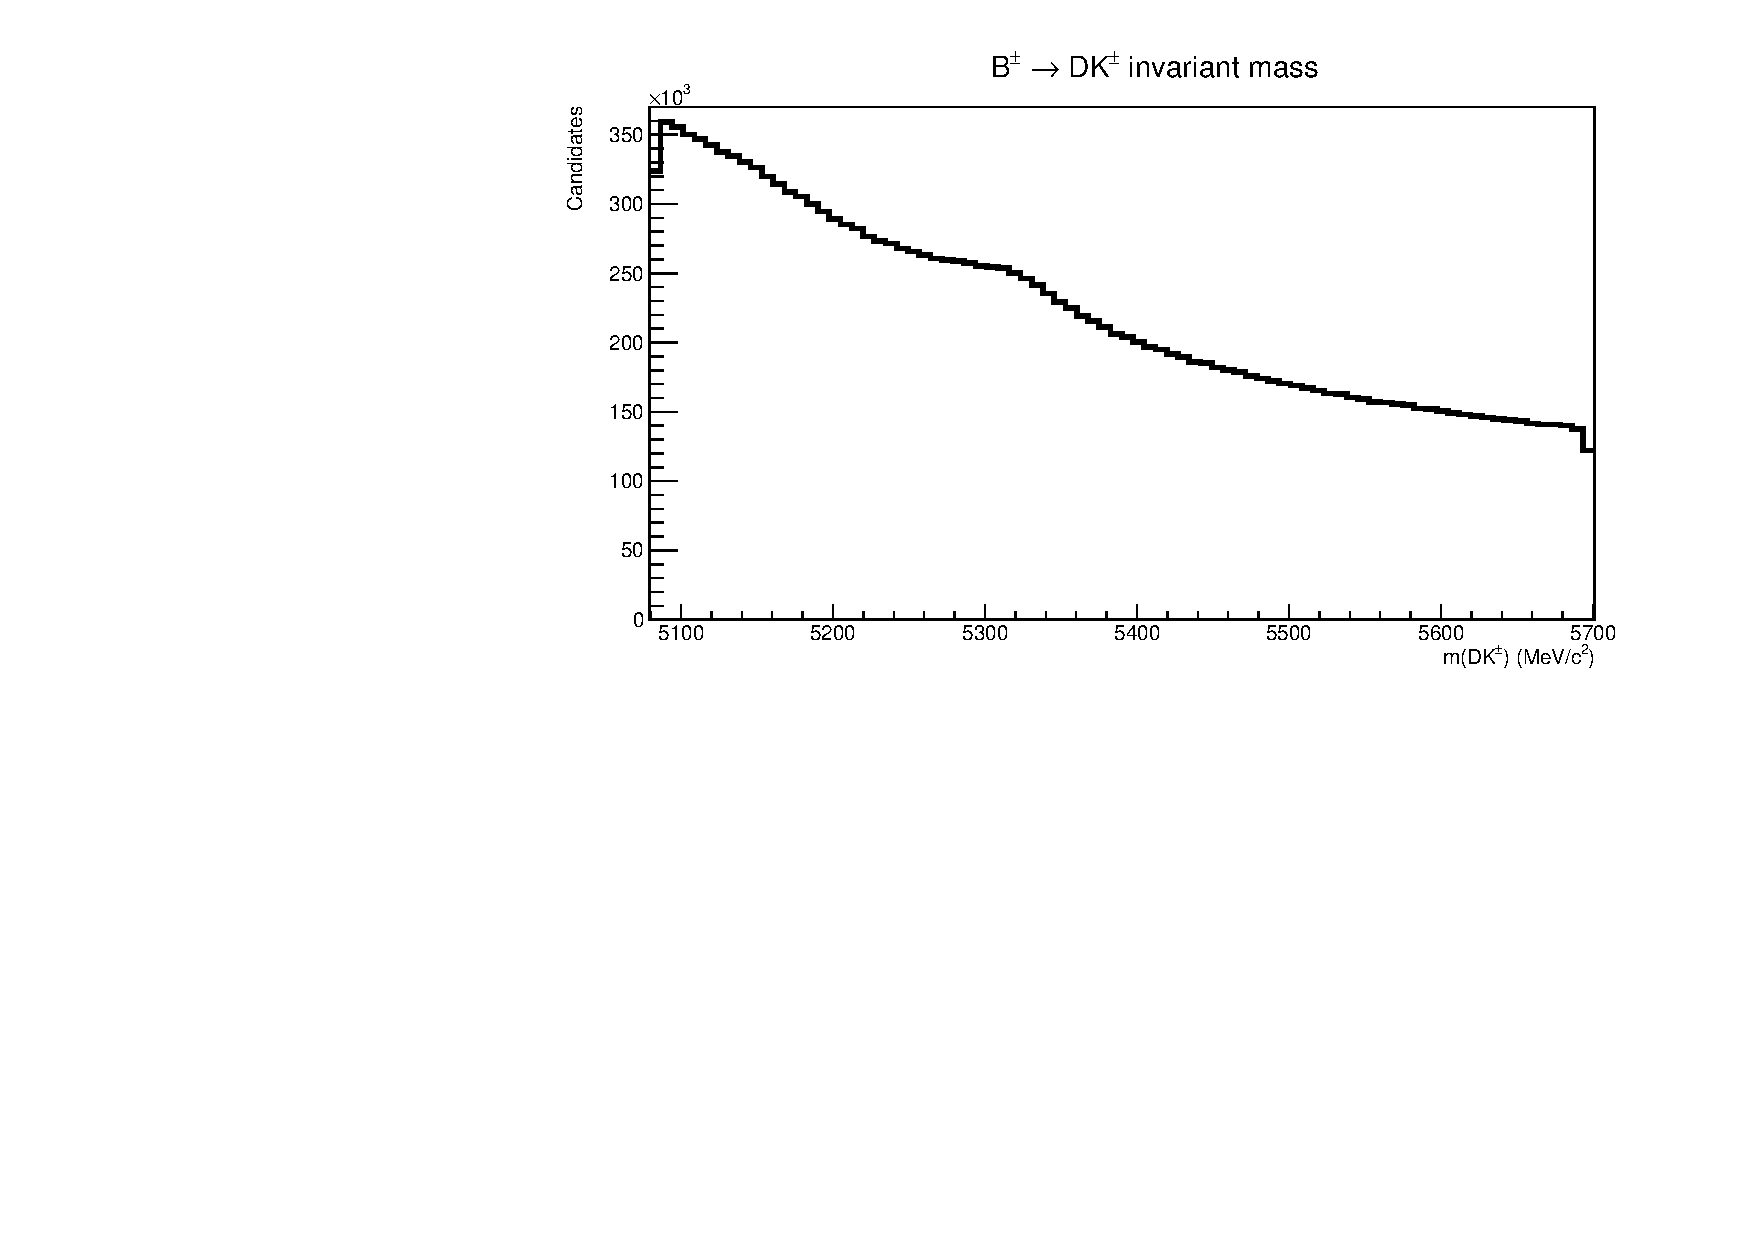
\includegraphics[width = 1.0\textwidth]{Plots/BmassStripping.pdf}
  \end{figure}
  \begin{center}
    The invariant $B$ mass, after online selection, show no visible signal...
  \end{center}
\end{frame}

\begin{frame}{Event selection}
  \begin{figure}
    \centering
    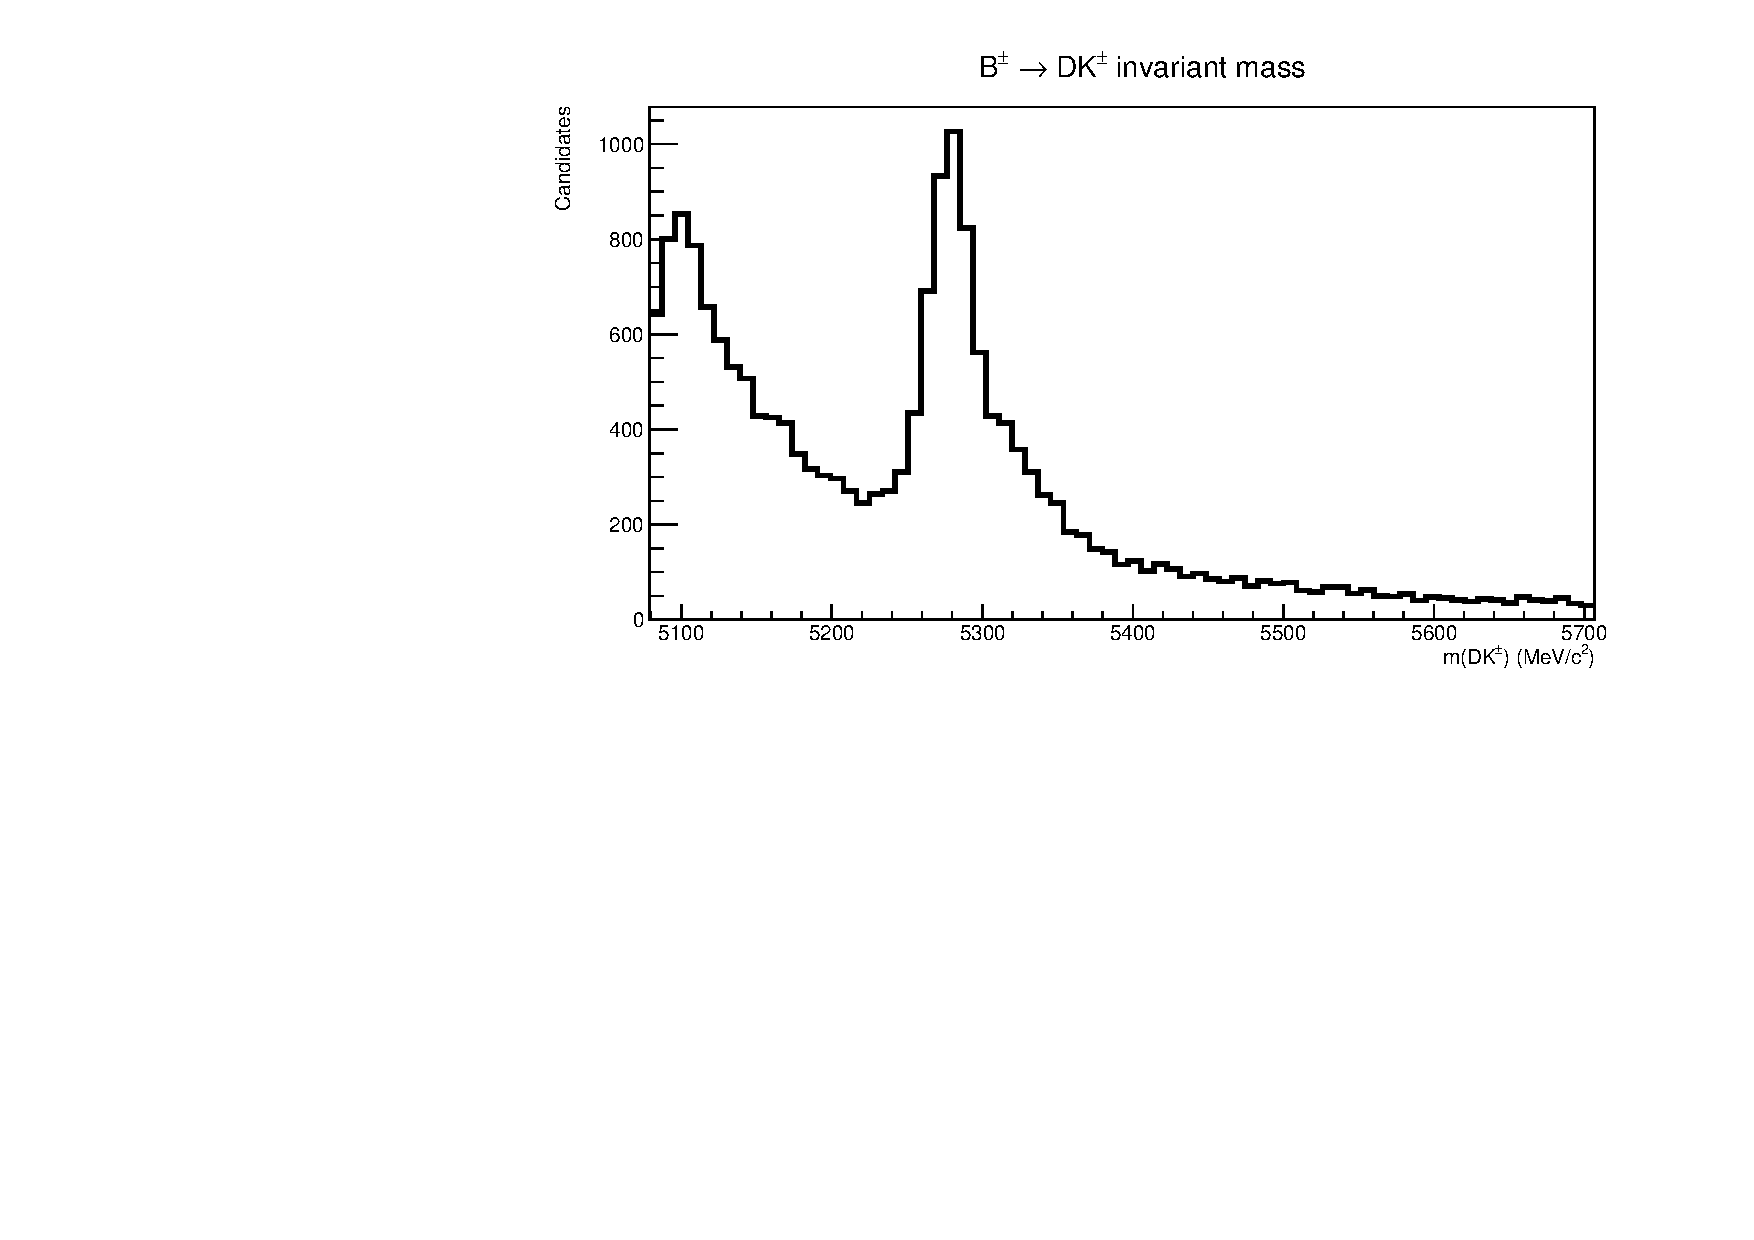
\includegraphics[width = 1.0\textwidth]{Plots/BmassFinalSelection.pdf}
  \end{figure}
  \begin{center}
    ... but the BDT does a great job cleaning this up!
  \end{center}
\end{frame}

\end{document}
